\documentclass[x11names,11pt,a4paper]{ctexart}
%以下为所使用的宏包
\usepackage{ulem}%下划线
\usepackage{amsmath,amsfonts,amssymb,amsthm,amsbsy}%数学符号
\usepackage{graphicx}%插入图片
\usepackage{booktabs}%三线表
%\usepackage{indentfirst}%首行缩进
\usepackage{tikz}%作图
\usetikzlibrary{shapes,arrows,chains}
\usepackage{appendix}%附录
\usepackage{array}%多行公式/数组
\usepackage{tabularx}%绘制定宽表格
\usepackage{makecell}%表格缩并
\usepackage{siunitx}%SI单位
\usepackage{mathrsfs}%数学字体
\usepackage{enumitem}%列表间距
\usepackage{multirow}%列表横向合并单元格
\usepackage[colorlinks,linkcolor=red,anchorcolor=blue,citecolor=green]{hyperref}%超链接引用
\usepackage{float}%图片、表格位置排版
\usepackage{pict2e,keyval,fp,diagbox}%带有斜线的表格
\usepackage{fancyvrb,listings}%设置代码插入环境
\usepackage{minted}%代码环境设置
\usepackage{fontspec}%字体设置
\usepackage{color,xcolor}%颜色设置
\usepackage{titlesec}%标题格式设置
\usepackage{makeidx}\makeindex%索引 编译命令 makeindex summary.idx
\usepackage{authblk}%titlepage作者信息



%页边距设置
\usepackage[left=0.5in,right=0.5in,top=0.7in,bottom=0.57in]{geometry}

%段行设置
\linespread{1.4}%行距
\setlength{\parskip}{0.1\baselineskip}%段距
\setlength{\parindent}{2em}%缩进

%字体设置
\setmainfont{Times New Roman}
\newfontfamily\consolas{Consolas}

%其他设置
\numberwithin{equation}{section}%公式按照章节编号
\newenvironment{point}{\raggedright$\Box $ }{}%新环境,用于标示重点内容
\newenvironment{rcode}{\raggedright$  \vartriangleright  $ \lstinline|R.| \textbf{Code}  \\}{}%新环境,用于建立R语言命令段落
\newcolumntype{Y}{>{\centering\let\newline\\\arraybackslash\hspace{0pt}}X}%tabularx中的居中表格格式
\allowdisplaybreaks[2]%跨页公式

%代码环境\lst设置
\definecolor{CodeBlue}{HTML}{268BD2}
\definecolor{CodeBlue2}{HTML}{0000CD}
\definecolor{CodeGreen}{HTML}{2AA1A2}
\definecolor{CodeRed}{HTML}{CB4B16}
\definecolor{CodeYellow}{HTML}{B58900}
\definecolor{CodePurPle}{HTML}{D33682}
\definecolor{CodeGreen2}{HTML}{859900}
\lstset{
    language=R,
    basicstyle=\fontspec{Consolas},
    numbers=left, %设置行号位置
    numberstyle=\tiny\color{black}, %设置行号大小
    keywordstyle=\color{black}, %设置关键字颜色
    stringstyle=\color{gray}, %设置字符串颜色
    commentstyle=\color{CodeGreen}, %设置注释颜色
    frame=single, %设置边框格式
    escapeinside=``, %逃逸字符(1左面的键),用于显示中文
    %breaklines, %自动折行
    extendedchars=false, %解决代码跨页时,章节标题,页眉等汉字不显示的问题
    xleftmargin=2em,xrightmargin=2em, aboveskip=1em, %设置边距
    tabsize=4, %设置tab空格数
    showspaces=false, %不显示空格
    emph={TRUE,FALSE,NULL,NAN,NA,\$,<-,T,F,:},emphstyle=\color{CodeBlue2}, %其他高亮
}

%节标题格式设置
\titleformat{\section}[block]{\centering\Large\bfseries}{Chapter. \Roman{section} }{1em}{}[]
\titleformat{\subsection}[block]{\Large\bfseries}{Section \arabic{section}.\arabic{subsection}}{1em}{}[]
% \titleformat{\subsubsection}[block]{\normalsize\bfseries}{    \arabic{subsection}-\alph{subsubsection}}{1em}{}[]
% \titleformat{\paragraph}[block]{\small\bfseries}{[\arabic{paragraph}]}{1em}{}[]

% \\titleformat{\\sectioncommand}[shape]{format}{title-label}{sep}{before-title}[after-title]


%SumatraPDF反向搜索命令行
%"C:\Users\彭拓锐Vincent\AppData\Local\Programs\Microsoft VS Code\Code.exe" "C:/Users/彭拓锐Vincent/AppData/Local/Programs/Microsoft VS Code\resources\app\out\cli.js" -r -g "%f:%l"




\begin{titlepage}
    \title{\textbf{A Brief Summary of Statistics Course}\\统计学课程知识总结}
  \author[]{Vincent\thanks{V1ncent19@outlook.com}}
    \affil[]{Department of Physics, Tsinghua University}
\end{titlepage}

\begin{document}

\maketitle\thispagestyle{myheadings}\markright{Complied using \LaTeX}

\tableofcontents
\newpage




% =================================================
% Set up a few colours
\colorlet{lcfree}{Green3}
\colorlet{lcnorm}{Blue3}
\colorlet{lccong}{Red3}
% -------------------------------------------------
% Set up a new layer for the debugging marks, and make sure it is on
% top
\pgfdeclarelayer{marx}
\pgfsetlayers{main,marx}
% A macro for marking coordinates (specific to the coordinate naming
% scheme used here). Swap the following 2 definitions to deactivate
% marks.
\providecommand{\cmark}[2][]{%
  \begin{pgfonlayer}{marx}
    \node [nmark] at (c#2#1) {#2};
  \end{pgfonlayer}{marx}
  } 
\providecommand{\cmark}[2][]{\relax} 
% -------------------------------------------------





\section{概率论部分}\label{Section1Probability}
\begin{center}
    Instructor: Wanlu Deng
\end{center}

%     Chapter Overview
% \begin{itemize}[topsep=2pt,itemsep=2pt]
%     \item \hyperlink{Basic axioms}{Basic axioms}
% \end{itemize}

    









%     Cover:Basic axioms, random events, $\sigma$-field; random variable/vector and their properties, some special distributions; $E$\,\&\,$\sigma^2$\,\&\,$cov$ and their properties; probability-generating/moment-generating/characteristic function; weak/strong law of large number, central limit thm.; intro. to multivariate normal distribution.



\subsection{Some Important Distributions}\label{SectionImportantDistributions}

\begin{table}[htbp]
    \centering
    \begin{tabular}{c|cccc}
        \hline
        $X$&$p_X(k)\big/f_X(x)$&$\quad \mathbb{E}\quad$&$var$&MGF\\
        \hline
        $\mathrm{Bern} (p)$& &$p$&$pq$&$q+pe^s$\\
        $B (n,p)$&$C_n^k p^k(1-p)^{n-k}$&$np$&$npq$&$(q+pe^s)^n$\\
        $\mathrm{Geo} (p)$&$(1-p)^{k-1}p$&$\dfrac{1}{p}$&$\dfrac{q}{p^2}$&$\dfrac{pe^s}{1-qe^s}$\\
        $H(n,M,N)$&$\dfrac{C_M^kC_{N-M}^{n-k}}{C_N^n}$&$n\dfrac{M}{N}$&$\dfrac{nM(N-n)(N-M)}{N^2(n-1)}$&\\
        $P(\lambda)$&$\dfrac{\lambda^k}{k!}e^{-\lambda}$&$\lambda$&$\lambda$&$e^{\lambda(e^s-1)}$\\
        $U(a,b)$&$\dfrac{1}{b-a}$&$\dfrac{a+b}{2}$&$\dfrac{(b-a)^2}{12}$&$\dfrac{e^{sb}-e^{sa}}{(b-a)^s}$\\
        $N(\mu,\sigma^2)$&$\dfrac{1}{\sigma \sqrt{2\pi}}e^{-\frac{(x-\mu)^2}{2\sigma^2}}$&$\mu$&$\sigma^2$&$e^{\frac{\sigma^2s^2}{2}+\mu s}$\\
        $\epsilon(\lambda)$&$\lambda e^{-\lambda x}$&$\dfrac{1}{\lambda}$&$\dfrac{1}{\lambda^2}$&$\frac{\lambda}{\lambda-s}$\\
        $\Gamma(\alpha,\lambda)$&$\dfrac{\lambda^\alpha}{\Gamma(\alpha)}x^{\alpha-1}e^{-\lambda x}$&$\dfrac{\alpha}{\lambda}$&$\dfrac{\alpha}{\lambda^2}$&$\left(\frac{\lambda}{\lambda-s}\right)^\alpha $\\
        $B(\alpha,\beta)$&$\dfrac{1}{B(\alpha,\beta)}x^{\alpha-1}(1-x)^{\beta-1}$&$\dfrac{\alpha}{\alpha+\beta}$&$\dfrac{\alpha\beta}{(\alpha+\beta)^2(\alpha+\beta+1)}$&\\
        $\chi^2_n$&$\dfrac{1}{2^{\frac{n}{2}}\Gamma(\frac{n}{2})}x^{\frac{n}{2}-1}e^{-\frac{x}{2}}$&$n$&$2n$&$ (1-2s)^{-n/2} $\\
        $t_\nu$&$\dfrac{\Gamma(\frac{\nu+1}{2})}{\sqrt{\nu\pi}\Gamma(\frac{\nu}{2})}(1+\frac{x^2}{\nu})^{-\frac{\nu+1}{2}}$&$0$&$\dfrac{\nu}{\nu-2}$&\\
        $F_{m,n}$&$\dfrac{\Gamma(\frac{m+n}{2})}{\Gamma(\frac{m}{2})\Gamma(\frac{n}{2})}\dfrac{m^\frac{m}{2}n^\frac{n}{2}x^{\frac{m}{2}-1}}{(mx+n)^{\frac{m+n}{2}}}$&$\dfrac{n}{n-2}$&$\dfrac{2n^2(m+n-2)}{m(n-2)^2(n-4)}$&\\
        \hline
    \end{tabular}
\end{table}

    Definition of PGF, MGF, CF see \autoref{SectionPGFMGFCF}.

    More Properties of $\chi^2,t,F$ see {\autoref{chi2_t_F_properties}}.

    Relation between distributions and more properties see \url{http://www.math.wm.edu/~leemis/chart/UDR/UDR.html}. Distribution support in \lstinline|R.| see \url{https://CRAN.R-project.org/view=Distributions}

Use the following command for all distributions supported in \lstinline|R. stats::|.
\begin{lstlisting}[language=R]
?Distributions
\end{lstlisting}


\subsection{Probability and Probability Model}

    What is \textbf{Probability}? A `belief' in `what would happen'.


\subsubsection{Sample Space and $\sigma$-Field}

\begin{point}
    Experiment and Sample Space
\end{point}

    Def. sample space $\Omega$: The set of \text{all} possible outcomes of one particular \textbf{experiment} . Conducting the experiment would result in a result/sample point $ \omega  $ in sample space $ \Omega  $. These results should be mutually exclusive, e.g. Tossing two coins simultaneously, the sample space is the set of all possible results
    \begin{align}
        \Omega = \{(0,0),(0,1),(1,0),(1,1)\}, \quad \omega \in \Omega 
    \end{align}

    On the sample space, the `belief' in results happening is measured by probability $ \mathbb{P}\left( \omega  \right),\,\omega \in\Omega   $

    \textbf{Note}: Randomness comes from the random result $ \omega  $ that an experiment generates.
    
\begin{point}
    Event 
\end{point}

    We may care about a conbination of some results, say `at least one of the coin lands tails-up'. It's like a kind of `structure' on sample space describing how we put results together to form \textbf{Events}. The definition is \index{Sigma-field@$ \sigma $-Field} a $\sigma$-field(or a $\sigma$-algebra) $\mathscr{F}$ as a collection of some subsets of $\Omega$, with properties:
    \begin{itemize}[topsep=2pt,itemsep=0pt]
        \item $\Omega\in\mathscr{F}$
        \item if $A\in\mathscr{F}$,then $A^\complement \in\mathscr{F}$
        \item if $A_n\in\mathscr{F}$, then ${\displaystyle\bigcup_{n=1}^\infty} A_n\in\mathscr{F}$
    \end{itemize}

    And $(\Omega,\mathscr{F})$ is a measurable space, on which we can select the events that we care about.

    Events (and their properties) can be described in the language of set, e.g. for events $ A $, $ B\in\mathscr{F} $
\begin{itemize}[topsep=2pt,itemsep=0pt]
    \item $ A=B $ means they are the same event
    \item $ A\cup B $ means one of them happens
    \item $ A\cap B $ or $ AB $ means both happen 
\end{itemize}

And some more complex ones
\begin{itemize}[topsep=2pt,itemsep=0pt]
    \item $ A\cup B=B\cup A $, $ A\cap B=B\cap A $
    \item $ A\cup (B\cup C)=A\cup B\cup C $, $ A\cap (B\cap C)=A\cap B\cap C $
    \item $ A\cap (B\cup C)=(A\cap B)\cup (B\cap C) $, $ A\cup (B \cap C)=(A\cup B)\cap (A\cup C) $
    \item $ A\cup B=A+ A^\complement\cap B $, $ A=A\cap B+A\cap B^\complement $
    \item[$ \Delta  $] $ (A\cup B)^\complement =A^\complement\cap B^\complement $, $ (A\cap B)^\complement = A^\complement \cup B^\complement  $
    \item $ (\bigcup_{j=1}^\infty A_j)^\complement =\bigcap_{j=1}^\infty A_j^\complement $
    \item $ (\bigcap_{j=1}^\infty A_j)^\complement =\bigcup_{j=1}^\infty A_j^\complement $
\end{itemize}
    
\subsubsection{Axioms of Probability}

    $\mathbb{P}(\,\cdot\,):\,\mathscr{F}\mapsto [0,1]$ is the probability measure (or probability function) defined on $(\Omega,\mathscr{F})$ describing the possibility that some event $ A\in\mathscr{F}  $ happens. Definition of probability $ \mathbb{P}(A) $ in useful models:
    \begin{align}
       \mathbb{P}\left( A \right) :=\begin{cases}
            \dfrac{\#A}{\#\Omega }&\text{Classical Model}\\
            \dfrac{m(A)}{m(\Omega )}&\text{Geometric Model}
        \end{cases}   
    \end{align}
    
    Where $ m(\, \cdot \, ) $ is some measure of events in continuous space, say integral in Euclidean Space $ \mathbb{R}^r $
    \begin{align}
        m_\mathrm{\mathbb{R}^r}(A)=\int_A \,\mathrm{d}x_1\,\mathrm{d}x_2\ldots\,\mathrm{d}x_r  
    \end{align}
    
    
    
    

    
    
    
\begin{point}
    Basic Axioms of Probability Mearure $ \mathbb{P}(\,\cdot\,) $
\end{point}

\begin{itemize}[itemsep=2pt,topsep=-2pt]
\item Non-negativity
\begin{equation}    \mathbb{P}(A)\geq 0\qquad \forall A\in\Omega    
\end{equation}
\item Normalization\footnote{Note: In other sections when dealing with not-yet-normalized distribution (say in Bayesian statistics), I usually use $ Z $ as the normalize constant, following the tradition in statistical physics where $ Z $ is the partition function.
\begin{align}
    \mathbb{P}=\dfrac{1}{Z}\tilde{\mathbb{P}},\quad Z=\int \mathbb{\tilde{P}} 
\end{align}}
\begin{equation}    \mathbb{P}(\Omega)=1    
\end{equation}




\item Countable Subadditivity\index{Countable Additivity}
\begin{equation}    \mathbb{P}(A_1\cup A_2\cup\cdots)=\mathbb{P}(A_1)+\mathbb{P}(A_2)+\cdots\quad ,\, (A_i\bot\!\!\!\bot  A_j\quad \forall i\neq j)
\end{equation}

where `countable subadditivity' means the events can be sequentially listed. e.g. $ [0,1]=\bigcup _{x\in [0,1]}\{x\} $ is not countable, intuition:
\begin{align}
    1=\mathbb{P}\left( [0,1] \right)=\mathbb{P}\left( \bigcup _{x\in [0,1]}\{x\} \right)   {\color{red}\neq} \sum_{x\in[0,1]}\mathbb{P}\left( x \right) =0
\end{align}


\end{itemize}

    Then $(\Omega,\mathscr{F},\mathbb{P})$ is probability space\index{Probability Space}, where $ \Omega  $ for experiment outcomes and randomness, $ \mathscr{F} $ for events and their algebra, $ \mathbb{P} $ for probability measure.

\begin{point}
        Properties of Probability:
\end{point}

    \begin{itemize}
        \item Addition Formula
        \begin{align}
            \mathbb{P}\left( A\cup B \right) =\mathbb{P}\left( A \right) +\mathbb{P}\left( B \right) -\mathbb{P}\left( A\cap B \right)  
        \end{align}
        \item Monotonicity
        \begin{equation}    
            \mathbb{P}(A)\leq \mathbb{P}(B)\quad \text{for}\, A\subset B
        \end{equation}
        \item Finite Subadditivity (Boole Inequality)\index{Inequality!Boole Inequality}
        \begin{equation}    
            \mathbb{P}(\bigcup_{i=1}^nA_i)\leq\sum_{i=1}^n \mathbb{P}(A_i)    
        \end{equation}
        \item Countable Subadditivity ($ \sigma  $-Subadditivity)\index{Sigma-Subadditivity@$ \sigma  $-Subadditivity}
        \begin{align}
            \mathbb{P}(\bigcup_{i=1}^\infty A_i)\leq\sum_{i=1}^\infty \mathbb{P}(A_i)  
        \end{align}
        
        
        \item Inclusion-Exclusion Formula (Jordan Formula)\index{Inclusion-Exclusion Formula}\index{Jordan Formula}
        \begin{align}
            \mathbb{P}(\bigcup_{i=1}^nA_i)=&\sum_{1\leq i\leq n}\mathbb{P}(A_i)-\sum_{1\leq i<j\leq n}\mathbb{P}(A_i\cap A_j)\\
            &+\sum_{1\leq i<j<k\leq n}\mathbb{P}(A_i\cap A_j\cap A_k)-\cdots\\
            &+(-1)^{n-1}\mathbb{P}(A_1 \cap A_2\cap\cdots \cap A_n)
        \end{align}

        Or in condensed notation:
        \begin{align}
            \mathbb{P}( \bigcup_{i=1}^n A_i)=&\sum_{k=1}^n (-1)^{k-1}\sum_{1\leq j_1<j_2<\ldots<j_k\leq n}\mathbb{P}\left( A_{j_1}\cap A_{j_2}\cap\ldots\cap A_{j_k} \right)   
        \end{align}
        
        
        \item Borel-Cantelli Lemma\index{Borel-Cantelli Lemma}
        \begin{align}
            &\sum_{n=1}^\infty \mathbb{P}(A_n)<\infty\Rightarrow \mathbb{P}(\lim_{n\to\infty}\sup A_n)=0\\
            &\sum_{n=1}^\infty \mathbb{P}(A_n)=\infty\Rightarrow \mathbb{P}(\lim_{n\to\infty}\sup A_n)=1\quad \text{if }A_i\text{ independent}
        \end{align}
            
    \end{itemize}


\begin{point}
    An Example 
\end{point}

    We have $ n $ different balls. Draw $ m $ times with replacement. What is the number of results regardless of order the balls drawn (e.g. $ \{\mathrm{red,red,black} \} $ is the same as $ \{\mathrm{red,black,red} \} $)? 

    The model is the same as we are `voting' for $ n $ different balls, with total ballot ticket $ m $. The $ m $ tickets are divided by $ n-1 $ plates (making them similar to ballot boxes), e.g. here's a $ n=4,m=6 $ vote corresponding to a result $ \omega \in\Omega  $:
    \begin{align}
         \bullet  \big|  \big| \bullet \bullet \bullet \big|  \bullet \bullet 
    \end{align}

    which the same as inserting plates sequentially and then cancel the order of plates:
    \begin{align}
        \# \Omega  = (m+1)*(m+2)\ldots (m+n-1)\bigg/ (n-1)! = \dfrac{(n+m-1)!}{m!(n-1)!}=\binom{n+m-1}{m}
    \end{align}

    (The idea of spacer plate is quite useful in dealing with some troublesome discrete cases, I think.)
    
    \begin{table}[H]
        \centering
        \renewcommand\arraystretch{1}
        \caption{$ \# \Omega  $ of Sampling $ n $ balls $ m $ draw}
        \begin{tabular}{ccc}
            \hline
            \hline
            &\multicolumn{2}{c}{Replacement}\\
            \cline{2-3}
            &With&Without\\
            \hline
            Ordered&$ n^m $&$ A_{n}^m $\\
            Unordered&$ \binom{n+m-1}{m} $&$ \binom{n}{m} $\\
            \hline
            \hline
        \end{tabular}
        \label{}
    \end{table}


    
    
    


\subsubsection{Conditional Probability}
    Motivation: To update the knowledge of probability measure.

    Def. \textbf{Conditional Probability} of $B$ given $A$:
    \begin{equation}    
        \mathbb{P}(B|A)=\frac{\mathbb{P}(A\cap B)}{\mathbb{P}(A)}    
    \end{equation}

    Actually it's a change of $\sigma$-field: $\Omega$ $ \to $ $B$
    \begin{align}
        \mathbb{P}\left( B|A \right) = \dfrac{m(B)}{m(A)} 
    \end{align}


\begin{point}
    Application of conditional probability:
\end{point}

        \begin{itemize}
        \item Multiplication Formula
        \begin{equation}    
            \mathbb{P}(\bigcap_{i=1}^n A_i)=\mathbb{P}(A_1)\prod_{i=2}^n \mathbb{P}(A_i|A_1\cap A_2\cap \cdots\cap A_{i-1})    
        \end{equation}
        \item Total Probability Thm.\index{Total Probability Thm.}
        \begin{equation}    
            \mathbb{P}(B)=\sum_{i=1}^n \mathbb{P}(A_i)\mathbb{P}(B|A_i)  
        \end{equation}
        where $\{A_i\}$ is a partition of $\Omega$: $ \Omega =\bigcup_{i}A_i ,\, A_i\cap A_j=\delta _{ij}\emptyset$

        (Actually just $ B\subset \bigcup_{i}A_i $ is enough, similar for Bayes's rule)
        \item Bayes's Rule\index{Bayes's Rule}
        \begin{equation}    
            \mathbb{P}(A_i|B)=\dfrac{\mathbb{P}(A_i)\mathbb{P}(B|A_i)}{\sum_{j=1}^n\mathbb{P}(A_j)\mathbb{P}(B|A_j)}    ,\quad 1\leq i\leq n
        \end{equation}
        where $\{A_i\}$ is a partition of $\Omega$: $ \Omega =\bigcup_{i}A_i,\, A_i\cap A_j=\delta _{ij}\emptyset $
    \end{itemize}

\subsubsection{Independency}
    Statistical Independency is defined as:
    \begin{equation}    
        A\independent B:\,\mathbb{P}(A\cap B) =\mathbb{P}(A)\mathbb{P}(B)
    \end{equation}

    Properties
    \begin{itemize}[topsep=2pt,itemsep=0pt]
        \item Complement set and indepency
        \begin{align}
            A\independent B\Leftrightarrow A^\complement \independent B 
        \end{align}
        \item Independency of multiple events
        \begin{align}
            A_1\independent A_2\independent\ldots \independent A_n \Leftrightarrow &\mathbb{P}\left( A_{j_1}\cap A_{j_2}\cap\ldots\cap A_{j_k} \right)=\mathbb{P}\left( A_{j_1} \right) \mathbb{P}\left( A_{j_2} \right) \ldots \mathbb{P}\left( A_{j_k} \right) \\
            &  \,\forall 1\leq j_1\leq j_2\leq \ldots \leq j_k\leq n\quad \forall k\leq n,\quad n<\infty
        \end{align}
    \end{itemize}
    
        

\subsection{Random Variable and Distribution}\label{SectionPropertiesOfRandomVariableAndVector}

Motivation: defining events is troublesome, and unhelpful to extract the key feature of events. A wise approach is to map samples \& events to numbers $ \Omega \mapsto \mathbb{R}^r $.

\subsubsection{Random Variable}
    Def. \text{Random Variable}: a \textbf{function}/mapping $X$ defined on sample space $\Omega$,  from $\Omega$ to some $\mathscr{X}\in\mathbb{R} $.
    \begin{align}
        X(\omega ):\, \Omega \mapsto \mathscr{X}\in\mathbb{R} 
    \end{align}

    \textbf{Note}: The mapping itself is non-random, the heart of randomness is still sample $ \omega  $ experimented. 

    Naturally $ X $ induces a mapping of probability measure
    \begin{align}
        F_X: \mathscr{X} \mapsto \Omega \mapsto \mathbb{P} 
    \end{align}

    To describe the mapping of probability, def. Cumulative Distribution Function (CDF)\index{CDF (Cumulative Distribution Function)}. (Here $ X(\omega ) $ is still used to remind the origin of randomness, in most case we simply use $ X $. )
    \begin{equation}
        F_X(x)=\mathbb{P} (X(\omega )\leq x)
    \end{equation}



    \begin{itemize}
        \item
        \begin{center}
            \parbox[t]{8.65cm}{PMF:\index{PMF (Probability Mass Function)}\begin{equation}        p_X(x)=F_X(x^+)-F_X(x^-)\end{equation}}
            \parbox[t]{8.65cm}{PDF:\index{PDF (Probability Density Function)}
            \begin{equation}        
                f_X(x)=\frac{\mathrm{d}F_X(x)}{\mathrm{d}x}
            \end{equation}}
        \end{center}
        \item Right-Continuity of CDF: A physical perspective is that PMF could be written as\footnote{Definition of Dirac $ \delta  $ function see \autoref{SubSubSectionFourierAndConvolution}.} 
        \begin{align}
            p_X(x)=\sum_{\tilde{x}\in\mathcal{X}}\mathbb{P}\left( X=\tilde{x} \right) \delta (x-\tilde{x})
        \end{align}
        where discrete $ X $ take values in $ \mathcal{X} $. In this way for any infinitesimal interval containing $ x $: $ \mathbb{I}_{x}\ni x$, we have 
        \begin{align}
            F_X(x^+)-F_X(x^-)=\int_{\mathbb{I}_{x}} p_X(x)\,\mathrm{d}x= \int_{\mathbb{I}_{x}}\sum_{\tilde{x}\in\mathcal{X}}\mathbb{P}\left( X=\tilde{x} \right) \delta (x-\tilde{x})\,\mathrm{d}x=\begin{cases}
                F_X(x^+)-F_X(x^-),&x\in \mathcal{X}\\
                0,&\text{others}
            \end{cases}
        \end{align}

        With such notation, in this note I sometimes ignore the difference between discrete cases / continuous cases.
        \item Representation of events: We could use random variable to express, say event $ A $ defined as        
        \begin{align}
            A:=\{\omega :X(\omega )\leq x\} 
        \end{align}
        
        
        \item Indicator function:\index{Indicator Function}
        \begin{equation}    
            \mathbb{I}_{x\in A}(x)=\begin{cases}
                1& x\in  A\\
                0& x\notin A
            \end{cases}
        \end{equation}
        \item Convolution\index{Convolution}
        \begin{itemize}
            \item $W=X+Y$
            \begin{equation}        
                f_W(w)=\int_{-\infty}^\infty f_X(x)f_Y(w-x)\mathrm{d}x    
            \end{equation}
            \item $V=X-Y$
            \begin{equation}        
                f_V(v)=\int_{-\infty}^\infty f_X(x)f_Y(x-v)\mathrm{d}x    
            \end{equation}
            \item $Z=XY$
            \begin{equation}        
                f_Z(z)=\int_{-\infty}^\infty \frac{1}{|x|}f_X(x)f_Y(\frac{z}{x})\mathrm{d}x
            \end{equation}
        \end{itemize}

            Examples:        
        \begin{itemize}[topsep=2pt,itemsep=0pt]
            \item Poisson\footnote{More about Poisson Distribution / Poisson Process see \autoref{SubSubSectionIndepedentProcess}}
            \begin{align}
                P(\lambda _1)+P(\lambda _2)\sim P(\lambda _1+\lambda _2) 
            \end{align}
            \item Binomial
            \begin{align}
                B(n_1,p)+B(n_2,p)\sim B(n_1+n_2,p) 
            \end{align}
            \item Gamma / Exponential
            \begin{align}
                \Gamma (\alpha _1,\lambda )+\Gamma (\alpha _2,\lambda )\sim \Gamma (\alpha _1+\alpha _2,\lambda ) 
            \end{align}
            with 
            \begin{align}
                \varepsilon (\lambda )=\Gamma (1,\lambda ) 
            \end{align}
            
            
            
            
            \item More relations of distributions see \url{http://www.math.wm.edu/~leemis/chart/UDR/UDR.html}
            \item Relation between Poisson Process and Exponential and Uniform distribution see \autoref{SubSubSectionPoissonProcess}.
            
            
        \end{itemize}
        
        \item Order Statistics\index{Order Statistics}\footnote{A relative object is Rank statistics, see \autoref{SubSectionIntroToNonParametricHypothesisTesting}.}
        
        Def $X_{(1)},X_{(2)},\cdots,X_{(n)}$ as order statistics of $\vec{X}$
        \begin{equation}    
            g_{X_{(i)}}=n!\prod_i f(x_i)\qquad \mathrm{for}\, x_1<x_2\cdots <x_n    
        \end{equation}
        PDF of $X_{(k)}$
        \begin{equation}\label{EqaDistributionOfOrderStatistics} 
            g_k(x_k)=nC_{n-1}^{k-1}[F(x_k)]^{k-1}[1-F(x_k)]^{n-k}f(x_k)
        \end{equation}
        \item $p$-fractile\index{Fractile!$ p $-fractile}
        \begin{equation}    \xi_p=F^{-1}(p)=\inf\{x|F(x)\geq p\}\end{equation}
    \end{itemize}






\subsubsection{Random Vector}
    A general case of random variable.\index{r.v. (Random Variable or Random Vector)} Its definition is similar    
    \begin{align}
        \vec{X}(\omega ):\, \Omega \mapsto \mathscr{X}\in\mathbb{R}^n 
    \end{align}
    a $n$-dimension Random Vector $\vec{X}=(X_1,X_2,\ldots,X_n)$ defined on $(\Omega,\mathscr{F},\mathbb{P})$.

    CDF $F(x_1,\ldots,x_n)$ defined on $\mathbb{R}^n$:
    \begin{equation}F(x_1,\ldots,x_n)=\mathbb{P}(X_1\leq x_1,\ldots,X_n\leq x_n)\end{equation}

    Joint PDF of random vector: 
    \begin{equation}
        f(x_1,\ldots,x_n)=\dfrac{\partial^n F(x_1,\ldots,x_n)}{\partial x_1\ldots\partial x_n}
    \end{equation}

    $k$-dimensional Marginal Distribution: For $1\leq k<n$ and index set $S_k=\{i_1.\ldots,i_k\}$, distribution of $\vec{X}=(X_{i_1},X_{i_2},\ldots,X_{i_k})$
    \begin{equation}F_{S_k}(X_{i_1}\leq x_{i_1},X_{i_2}\leq x_{i_2}\ldots,X_{i_k}\leq x_{i_k})=\mathbb{P}(X_{i_1}\leq x_{i_1},\ldots,X_{i_k}\leq x_{i_k};X_{i_{k+1}},\ldots,X_{i_n}\leq\infty)\end{equation}

    Marginal distribution: 
    \begin{equation}
        g_{S_k}(x_{i_1},\ldots,x_{i_k})=\int_{\mathbb{R}^{n-k}}f(x_1,\ldots,x_n)\mathrm{d}x_{i_{k+1}}\ldots\mathrm{d}x_{j_n}=\dfrac{\partial^{n-k}F(x_1,\ldots,x_n)}{\partial x_{i_{k+1}}\ldots\partial x_{i_n}}
    \end{equation}


    \begin{itemize}
        \item[$\Delta$] \textbf{Function of r.v.}
        
        For $\vec{X}=(X_1,X_2,\cdots,X_n)$ with PDF $f(\vec{X})$ and define 
        \begin{equation}    
            \vec{Y}=(Y_1,Y_2,\cdots,Y_n)=\left(y_1(\vec{X}),y_2(\vec{X}),\cdots,y_n(\vec{X})\right)
        \end{equation}
        with inverse mapping
        \begin{equation}    
            \vec{X}=(X_1,X_2,\cdots,X_n)=\left(x_1(\vec{Y}),x_2(\vec{Y}),\cdots,x_n(\vec{Y})\right)
        \end{equation}
        then
        \begin{equation}    
            g(\vec{Y})= f\left(x_1(\vec{Y}),x_2(\vec{Y}),\cdots,x_n(\vec{Y})\right)\left|\frac{\partial \vec{X}}{\partial\vec{Y}}\right|\mathbb{I}_{D_Y}
        \end{equation}

        (Intuitively: $g(\vec{Y} )\mathrm{d}\vec{Y}=\mathrm{d}\mathbb{P}=f(\vec{X})\mathrm{d}\vec{X}$)
    \end{itemize}



    




\subsection{Expectation $\mathbb{E}$, Variance $var$ and Covariance $cov$}
Motivation: what would happen `on average'?

Expectation and Variance of common distributions see \autoref{SectionImportantDistributions}.

\subsubsection{Expection $ \mathbb{E}(\,\cdot\,) $}
    Expectation of r.v. $g(X)$ def.:
    \begin{equation}
    \mathbb{E} [g(X)]=\begin{cases}
        {\displaystyle\int_\Omega g(x) f_X(x)\mathrm{d}x=\int_\Omega g(x)\mathrm{d}F(x)}\\
        {\displaystyle\sum_{\Omega}g(x)f_X(x)}
    \end{cases}
\end{equation}

    Sometimes when there are more than 1 variables, say $ x,y $, we would use notation $ \mathbb{E}_X\left( g(X,Y) \right)  $ to specify the variable to avoid confusion.

    \textbf{Note}: For discrete r.v. the expectation always exists, but for continuous \& unbounded r.v. the expectation might diverge, rigorously speaking:
    \begin{align}
        \mathbb{E}\left[ X \right]\exists:\, \int_{\mathbb{R}}|x|f(x)\,\mathrm{d}x<\infty  
    \end{align}
    
    
 
\begin{point}
    Properties of Expectation $E(\,\cdot\,)$:
\end{point}

\begin{itemize}
    \item Linearity of Expectation\begin{equation}
        \mathbb{E}(aX+bY)=a \mathbb{E}(X)+b\mathbb{E}(Y)
    \end{equation}
    \item Conditional Expectation\begin{equation}
        \mathbb{E}(X|A)=\frac{\mathbb{E}(X\mathbb{I}_A)}{\mathbb{P}(A)}
    \end{equation}
    
    Note: if take $A$ as $Y$ is also a r.v. then conditional expectation is actually a function of $Y$
    \begin{equation}\xi (Y)=\mathbb{E}(X|Y)=\int xf_{X|Y}(x)\mathrm{d}x\end{equation}

    

    \item Law of Total Expectation\begin{equation}
        \mathbb{E}_Y\big\{\mathbb{E}_X[g(X)|Y]\big\}=\mathbb{E}_X[g(X)]
    \end{equation}
    \item r.v.\& Event
    \begin{equation}
        \mathbb{P}(A|X)=\mathbb{E}(\mathbb{I}_A|X)\Rightarrow \mathbb{E}[P(A|X)]=\mathbb{E}(\mathbb{I}_A)=\mathbb{P}(A)
    \end{equation}
    \item Conditional Expectation
    \begin{equation}
        \mathbb{E}\big[h(Y)g(X)|Y\big]=h(Y)\mathbb{E}[g(X)|Y]
    \end{equation}
\end{itemize}


\subsubsection{Variance $ var(\, \cdot \, ) $}
    Variance of r.v. $X$: 
    \begin{equation}
        var(X)=\mathbb{E}\big[(X-\mathbb{E}(X))^2\big]=\mathbb{E}(X^2)-(\mathbb{E}(X))^2
    \end{equation}
    (sometimes denoted as $\sigma^2_X$.)

    Another definition comes from the MMSE estimation, 
    \begin{align}
        var(X)=\mathop{\min}\limits_{c}\mathbb{E}\left[ (X-c)^2 \right]   
    \end{align}
    
    its solution is $ c=\mathbb{E}\left[ X \right]  $. See \autoref{SubSecMMSE} for more.

\begin{point}
    Properties:
\end{point}

\begin{itemize} 
    \item Linear combination of Variance\begin{equation}
        var(aX+b)=a^2var(X)
    \end{equation}
    \item Conditional Variance
    \begin{equation}
        var(X|Y)=\mathbb{E}{[X-\mathbb{E}(X|Y)]^2|Y}
    \end{equation}
    \item Law of Total Variance\begin{equation}
        var(X)=\mathbb{E}[var(X|Y)]+var[\mathbb{E}(X|Y)]
    \end{equation}
\end{itemize}

    Standard Deviation def. as :
    \begin{equation}\sigma_X=\sqrt{var(X)}\end{equation}

    Then can construct \textbf{Standardization}\index{Standardization} of r.v.
    \begin{equation}X_\mathrm{sd} =\frac{X-\mathbb{E}(X)}{\sqrt{var(X)}}\end{equation}


\subsubsection{Covariance $ cov(\, \cdot \, ) $ and Correlation $ corr(\, \cdot \, ) $}\label{SubSubSectionCovarianceAndCorrelation}
    Covariance of r.v. $X$ and $Y$:\begin{equation}
        cov(X,Y)=\mathbb{E}\big[(X-\mu_X)(Y-\mu_Y)\big]=\mathbb{E}(XY)-\mathbb{E}(X)\mathbb{E}(Y)
    \end{equation}

    And Correlation Coefficient\index{Correlation Coefficient}
    \begin{equation}
        \rho_{X,Y}=corr(X,Y)=\frac{cov(X,Y)}{\sqrt{var(X)var(Y)}}
    \end{equation}

    Remark: correlation $\nRightarrow$ cause and effect. 
    Detail on causal effect topic see \autoref{SecCausalInference}.

    Properties:
\begin{itemize}
\item Bilinear of Covariance\begin{align}
    cov(X+Y,Z)&=cov(X,Z)+cov(Y,Z)\\
    cov(X,Y+Z)&=cov(X,Y)+cov(X,Z)
\end{align}
    
\item Variance and Covariance
\begin{equation}\label{EqaVarOfSumOfRV}
    var(X+Y)=var(X)+var(Y)+2cov(X,Y)
\end{equation}
\item Covariance Matrix\index{Covariance Matrix}

    Def $\Sigma=\mathbb{E}\big[(X-\mu)(X-\mu)^T\big]=\{\sigma_{ij}\}$ (where $X$ should be considered as a column vector)
\begin{equation}\label{covariancematrix}
    \Sigma=
        \begin{pmatrix}
        var(X_1) & cov(X_1,X_2) & \ldots & cov(X_1,X_n)\\
        cov(X_2,X_1) & var(X_2) & \ldots & cov(X_2,X_n)\\
        \vdots & \vdots & \ddots & \vdots\\
        cov(X_n,X_1) & cov(X_n,X_2) & \ldots & var(X_n)\\
        \end{pmatrix}    
    \end{equation}
\end{itemize}

Attachment: Independence:\begin{equation}    X_i \independent X_j\Rightarrow \begin{cases}
        f(x_1,x_2,\cdots,x_n)=\prod f(x_i)\\
        F(x_1,x_2,\cdots,x_n)=\prod F(x_i)\\
        E(\prod X_i)=\prod E(X_i)\\
        var(\sum X_i)=\sum var(X_i)
    \end{cases},\qquad n<\infty
\end{equation}


\subsection{PGF, MGF and C.F}\label{SectionPGFMGFCF}

    Generating Function: Representation of $\mathbb{P}$ in function space. $\mathbb{P}\Leftrightarrow$ Generating Function.

\subsubsection{Probability Generating Function}
    PGF\index{PGF (Probability Generating Function)}: used for non-negative, integer $X$, which is the $ z $-transform of $ p_X $
    \begin{equation}
        g(s)=\mathbb{E}(s^X)=\sum_{j=0}^\infty s^j\mathbb{P}(X=j)    ,s\in[-1,1]
    \end{equation}

\begin{point}
        Properties
\end{point}
    \begin{itemize}[topsep=2pt,itemsep=0pt]
        \item $\mathbb{P}(X=k)=\dfrac{g^{(k)}(0)}{k!}$
        \item $\mathbb{E}(X)=g^{(1)}(1)$
        \item $var(X)=g^{(2)}(1)+g^{(1)}(1)-[g^{(1)}(1)]^2 $
        \item For $X_1,X_2,\cdots,X_n$ independent with $g_i(s)=\mathbb{E}(s^{X_i})$, $Y={\displaystyle \sum_{i=1}^n} X_i$, then
        \begin{equation}    
            g_Y(s)=\prod_{i=1}^n g_i(s),s\in[-1,1]
        \end{equation}
        \item For ${X_i}$ i.i.d with $\psi_i(s)=\psi(s)\equiv \mathbb{E}(s^{X_i})$, $Y$ with $G(s)\equiv\mathbb{E}(s^{Y})$, $W=X_1+X_2+\cdots +X_Y$,then
        \begin{equation}    
            g_W(s)=G[\psi(s)]    
        \end{equation}
        \item 2-Dimensional PGF of $(X,Y)$
        \begin{equation}    
            g(s,t)=\mathbb{E}(s^Xt^Y)=\sum_{i=o}^\infty\sum_{j=0}^\infty \mathbb{P}_{(X,Y)}(X=i,Y=j)s^it^j,\quad s,t\in[-1,1]
        \end{equation}
    \end{itemize}
\subsubsection{Moment Generating Function}
    MGF\index{MGF (Moment Generating Function)}: used for non-negative $ X $, which is the Laplacian transformation of $ f_X $.
    \begin{equation}
        M_X(s)=\mathbb{E}(e^{sX})=\begin{cases}
            \sum_je^{sx}\mathbb{P}(X=x_j)\\
            \int_{-\infty}^\infty e^{sx}f_X(x)\mathrm{d}x
        \end{cases}
    \end{equation}

    Properties
    \begin{itemize}
        \item MGF of $Y=aX+b$: $
            M_Y(s)=e^{sb}M(sa)    $
        \item $\mathbb{E}(X^k)=M^{(k)}(0)$
        \item $\mathbb{P}(X=0)={\displaystyle\lim_{s\to -\infty}}M(s)$
        \item For $X_1,X_2,\cdots,X_n$ independent with $M_{X_i}(s)=\mathbb{E}(e^{sX_i})$, $Y={\displaystyle \sum_{i=1}^n} X_i$, then
        \begin{equation}    
            M_Y(s)=\prod_{i=1}^n M_{X_i}(s)
        \end{equation}
    \end{itemize}
\subsubsection{Characteristic Function}
    C.F \index{C.F. (Characteristic Function)}is actually the Fourier Transform of $f_X$.
    \begin{equation}
        \phi(t)=\mathbb{E}(e^{itX}) = \int_{-\infty}^\infty e^{itx}f_X(x)\mathrm{d}x
    \end{equation}

    Properties
    \begin{itemize}
    \item if $E(|X|^k)<\infty$,then
    \begin{equation}
        \phi^{(k)}(t)=i^k\mathbb{E}(X^ke^{itX})\qquad \phi^{(k)}(0)=i^k\mathbb{E}(X^k)    
    \end{equation}
    \item For $X_1,X_2,\cdots,X_n$ independent with $\phi_{X_i}(t)=\mathbb{E}(e^{itX_i})$, $Y={\displaystyle \sum_{i=1}^n} X_i$, then
    \begin{equation}
        \phi_Y(t)=\prod_{i=1}^n \phi_{X_i}(t)
    \end{equation}
    \item Inverse (Fourier) Transform
    \begin{equation}
        f(x)=\frac{1}{2\pi}\int_{-\infty}^\infty e^{-itx}\phi(t)\mathrm{d}t    
    \end{equation}
\end{itemize}



\subsection{Convergence and Limit Distribution}
\subsubsection{Convergence Mode}
    \index{Convergence}
    \begin{equation}
        \begin{cases}
            \text{Convergence in Distribution }&{\displaystyle X_n\xrightarrow[]{\mathrm{d}}X:\lim_{n\to\infty}F_n(x)=F(x)}\\
            \text{Convergence in Probability }&{\displaystyle X_n\xrightarrow[]{\mathrm{p}}X:\lim_{n\to\infty}\mathbb{P}(|X_n-X)\geq\varepsilon)=0\, ,\forall\varepsilon>0}\\
            \text{Almost Sure Convergence }&{\displaystyle X_n\xrightarrow[]{\text{a.s.}}X:\mathbb{P}(\lim_{n\to\infty}X_n=X)=1}\\
            L_p\text{ Convergence }&{\displaystyle X_n\xrightarrow[]{L_p}X:\lim_{n\to\infty}\mathbb{E}(|X_n-X|^p)=0}
        \end{cases}
    \end{equation}

        Relations between convergence:
        \begin{center}
            \begin{tikzpicture}
                \draw(-1,-1)rectangle(1,1);
                \draw(-3,-0.5)rectangle(-5,-2.5);
                \draw(-3,0.5)rectangle(-5,2.5);
                \draw(3,-1)rectangle(5,1);
                \draw[-latex](-3,-1.5)--(-1,-0.5);
                \draw[-latex](-1,-0.75)--(-3,-1.75);
                \draw[-latex](-3,1.5)--(-1,0.5);
                \draw[-latex](1,0)--(3,0);
                \node at (0,0){$X_n\xrightarrow[]{\mathrm{p}}X$};
                \node at (-4,-1.5){$X_n\xrightarrow[]{L_p}X$};
                \node at (-4,1.5){$X_n\xrightarrow[]{\text{a.s.}}X$};
                \node at (4,0){$X_n\xrightarrow[]{\mathrm{d}}X$};
                \node at (-1.5,-1.5){$L_p<\infty $};
            \end{tikzpicture}
        \end{center}

        Note: $ L_2 $ convergence is also denoted m.s. (mean squared) convergence $ \xrightarrow[]{\mathrm{m.s.}}  $.

        Useful Thm.:
        \begin{itemize}
            \item Continuous Mapping Thm.: For continuous function $g(\cdot)$\index{Continuous Mapping Thm.}\hypertarget{ContinuousMapping}{}
            \begin{enumerate}
                \item $X_n\xrightarrow[]{\text{a.s.}}X\Rightarrow g(X_n)\xrightarrow[]{\text{a.s.}}g(X)$
                \item $X_n\xrightarrow[]{\mathrm{p}}X\Rightarrow g(X_n)\xrightarrow[]{\mathrm{p} }g(X)$
                \item $X_n\xrightarrow[]{\mathrm{d}}X\Rightarrow g(X_n)\xrightarrow[]{\mathrm{d}}g(X)$
            \end{enumerate}
            \item Slutsky's Thm.\index{Slutsky's Thm.}: For $X_n\xrightarrow[]{\mathrm{d}}X,Y_n\xrightarrow[]{\mathrm{p}}c$
            \begin{enumerate}
                \item $X_n+Y_n\xrightarrow[]{\mathrm{d}}X+c$
                \item $X_nY_n\xrightarrow[]{\mathrm{d}}cX$
                \item $X_n/Y_n\xrightarrow[]{\mathrm{d}}X/c$
            \end{enumerate}
            \item Continuity Thm. for characteristic function:
            \begin{equation}        \lim_{n\to\infty}\phi_n(t)=\varphi(t)\Leftrightarrow X_n\xrightarrow[]{\mathrm{d}}X\end{equation}
        \end{itemize} 


\subsubsection{Law of Large Number \& Central Limit Theorem}

\begin{itemize}
\item m.s. LLN\index{m.s. LLN (Mean-Squared Law of Large Number)}: For $ X_i $ with $ cov(X_i,X_j)=0$, if $ i\neq j $, and $ \mathbb{E}\left[ X_i \right] =\mu <\infty $
\begin{align}
    \frac{1}{n}\sum X_i\xrightarrow[]{L_2} \mathbb{E}\left[ X_1 \right]
\end{align}


\item WLLN\index{LLN (Law of Large Number)}\index{WLLN (Weak Law of Large Number)}: For $ X_i $ i.i.d. $ \sim f_X $, with $ \mathbb{E}\left[ X_i \right]=\mu <\infty $
\begin{equation}\label{EqaWLLN}    \frac{1}{n}\sum X_i\xrightarrow[]{\mathrm{p}}\mu 
\end{equation}
\item SLLN\index{SLLN (Strong Law of Large Number)}: For $ X_i $ i.i.d. $ \sim f_X $, with $ \mathbb{E}\left[ X_i \right] =\mu <\infty $
\begin{equation}    \frac{1}{n}\sum X_i\xrightarrow[]{\text{a.s.}}  \mu 
\end{equation}
\item CLT\index{CLT (Central Limit Thm.)}: For $ X_i $ i.i.d. $ \sim f_X $, with $ \mathbb{E}\left[ X_i \right] =\mu <\infty $, $ var(X_i)=\sigma ^2<\infty $
\begin{align}
     \dfrac{\sqrt{n}\left(\bar{X}-\mu \right)}{\sigma }\xrightarrow[]{\mathrm{d}} N(0,1)
\end{align}
or in equivalent form
\begin{align}    
    &\frac{1}{\sigma\sqrt{n}}\sum(X_k-\mu)\xrightarrow[]{\mathrm{d}} N(0,1)\\
    &\bar{X}\xrightarrow[]{\mathrm{d}} N(\mu ,\dfrac{\sigma ^2}{n})
\end{align}

\begin{proof}
    Denote the characteristic function of $ X\sim f_X(x) $ as $ \phi _X(t):=\mathbb{E}\left[ e^{itX} \right] $, with expectation $ \mu :=\mathbb{E}\left[ X \right]  $ and variance $ \sigma^2:=var(X)=\mathbb{E}\left[ X^2\right] -\mu  ^2 $.
    
    Define $ Z=\dfrac{X-\mu }{\sigma } $ The taylor series of $ \phi _Z(t) $ at $ t=0 $ yields:
    \begin{align*}
        \phi _Z(t)=1-\dfrac{t^2}{2}+o(t^2) 
    \end{align*}
    The characteristic function of mean $ \displaystyle\bar{Z}:=\dfrac{1}{n}\sum_{i=1}^nZ_i=\dfrac{1}{n}\sum_{i=1}^n\dfrac{X_i-\mu }{\sigma } $ w.r.t. $ X_i $ i.i.d. $ \sim f_X(x) $
    \begin{align*}
        \phi _{\bar{Z}}(t)=\mathbb{E}\left[ e^{it\bar{Z}} \right]=&\left[\phi _{Z}(\dfrac{t}{n})\right]^n=\left[1-\dfrac{t^2}{2n^2}\right] ^n 
    \end{align*}
    with $ n\to\infty $ limit:\footnote{Note: if use characteristic function of $ X_i $ directly, notice that
    \begin{align*}
        n\log\left(1+ \dfrac{at}{n}-\dfrac{bt^2}{2n^2}\right)= at -\left(b+a^2\right)\dfrac{t^2}{2n}+\mathcal{O}(\dfrac{1}{n^2})
    \end{align*}
    using the taylor series of $ \log(1+\xi ) $ at $ \xi =0 $.
    }
    \begin{align*}
        \lim_{n\to\infty}\phi _{\bar{Z}}(t)=&\lim_{n\to\infty} \left[1-\dfrac{1}{n}\dfrac{t^2}{2n}\right] ^n=e^{-\frac{t^2}{2n}} \Rightarrow \bar{Z}=\dfrac{\bar{X}-\mu }{\sigma }\xrightarrow[]{\mathrm{d}} N(0,\dfrac{1}{n})
    \end{align*}

\end{proof}

\item de Moivre-Laplace Thm.\index{de Moivre-Laplace Thm.} is a special case of CLT at $ S_n\sim B (n,p) $
\begin{equation}    \mathbb{P}(k\leq S_n\leq m)\approx \Phi(\frac{m+0.5-np}{\sqrt{npq}})-\Phi(\frac{k-0.5-np}{\sqrt{npq}})
\end{equation}
\item Stirling Eqa. derived from CLT
\begin{equation}    \frac{\lambda^k}{k!}e^{-\lambda}\approx \frac{1}{\sqrt{\lambda}\sqrt{2\pi}}e^{-\frac{(k-\lambda)^2}{2\lambda}}\xrightarrow[\lambda=n]{k=n}n!\approx\sqrt{2\pi n}(\frac{n}{e})^n\sim O\left((\dfrac{n}{e})^n\right)
\end{equation}

\end{itemize}


\subsection{Inequalities}\label{SubSectionUsefulInequality}
    
\begin{itemize}
    \item Cauchy-Schwarz Inequality\index{Inequality!Cauchy-Schwarz Inequality}
    \begin{equation}
        \left\vert \mathbb{E}(XY) \right\vert\leq \sqrt{\mathbb{E}(X^2)\mathbb{E}(Y^2)}
    \end{equation}

    \item Bonferroni Inequality\index{Inequality!Bonferroni Inequality}
\begin{equation}    \mathbb{P}(\bigcup_{i=1}^n A_i)\geq \sum_{1\leq i\leq n}  \mathbb{P}(A_i)+\sum_{1\leq i <j\leq n}  \mathbb{P}(A_i\cap A_j)
\end{equation}
    \item Markov Inequality\index{Inequality!Markov Inequality}
\begin{equation}     \mathbb{P}(|X|\geq \epsilon)\leq\frac{\mathbb{E}(|X|^\alpha)}{\epsilon^\alpha}
\end{equation}

    with $ \alpha =1 $, and $ \varepsilon  $ selected as a multiple of $ \mathbb{E}\left[ |X| \right]  $:
    \begin{align}
        \mathbb{P}\left( |X|\geq m\mathbb{E}\left[ |X| \right]  \right) \leq \dfrac{1}{m} 
    \end{align}
    
    
    \item Chebyshev Inequality\index{Inequality!Chebyshev Inequality}
\begin{equation}     \mathbb{P}(|X-\mathbb{E}(X)|\geq\epsilon)\leq\frac{var(X)}{\epsilon^2}
\end{equation}

    Chebyshev inequality is used to proof WLLN \autoref{EqaWLLN}
    \item Jensen Inequality\index{Jensen Inequality}: For convex function $h(x)$:\footnote{Or equivalently for concave function $ \tilde{h}(x) $:
    \begin{align}
         \mathbb{E}[\tilde{h}(X)]\leq \tilde{h}(\mathbb{E}(X))
    \end{align}
    }
\begin{equation}    \mathbb{E}[h(X)]\geq h(\mathbb{E}(X))
\end{equation}
    
    Example of using Jensen Eqa. to proof some other inequalities:
    \begin{itemize}[topsep=2pt,itemsep=0pt]
        \item Non-negativity of Kullback-Leibler Divergence: For two distributions $ f(\, \cdot \, ) $ and $ g(\, \cdot \, ) $, the K-L Divergence is defined as 
        \begin{align}
            \mathrm{KL}(f\Vert g):=-\int f(x)\log \dfrac{g(x)}{f(x)}  \,\mathrm{d}x
        \end{align}
        
        Take $ h(\xi ):=\log \xi  $ a concave function for $ \xi \in(0,\infty) $ and $ Z:=\dfrac{g(X)}{f(X)} $ with $ X\sim f(x) $, then
        \begin{align}
            \mathbb{E}\left( h(Z) \right) =&\int _A \left(\log z\right) f_Z(z) \,\mathrm{d}z=\int _A \left(\log \dfrac{g(x)}{f(x)}\right) f(x) \,\mathrm{d}x\\
            \leq &h(\mathbb{E}\left( Z \right) )=\log \int _A zf_Z(z) \,\mathrm{d}z=\log \int _A \dfrac{g(x)}{f(x)}f(x) \,\mathrm{d}x=0\\
            \Rightarrow& -\int _A \log f(x)\dfrac{g(x)}{f(x)} \,\mathrm{d}x\geq 0
        \end{align}
        % \item Non-negativity of \hyperlink{NormDefinition}{$ \ell_p $ Norm}:
        % \begin{align}
        %     \left\Vert x \right\Vert _p= \left(\sum_{i=1}^n |x_i|^p \right)^{1/p},\quad p\geq 1
        % \end{align}
        
        % Take $ h(\xi ):=|\xi |^p  $ a convex function for $ p\geq 1 $ and r.v. $ Z_n $ is defined a discrete one with distribution
        % \begin{align}
        %     Z_n=x_1,x_2\,\ldots, x_n ,\,\mathrm{w.p.} \dfrac{1}{n}
        % \end{align}
        
        % i.e. $ Z_n $ has equal probability to be assigned value in $ \{x_1,x_2\,\ldots, x_n\} $. Then
        % \begin{align}
        %     \mathbb{E}\left( h(Z) \right) =&\sum_{i=1}^n\dfrac{1}{n}|x_i|^p\\
        %     \geq&h(\mathbb{E}\left( Z \right) )=\left|\sum_{i=1}^n\dfrac{1}{n}x_i\right|^p\\
        %     \Rightarrow & \left|\sum_{i=1}^nx_i\right|^p\leq n^{p-1}\sum_{i=1}^n\dfrac{1}{n}|x_i|^p,\quad p\geq 1
        % \end{align}
    \end{itemize}
    \item Cantelli Inequality\index{Cantelli Inequality}
    \begin{align}
        \mathbb{P}\left( X-\mathbb{E}\left[ X \right] \geq \lambda  \right) \leq \dfrac{var(X)}{var(X)+\lambda ^2} 
    \end{align}
    with $ \lambda =\sqrt{var(X)}:=\sigma  $, we have
    \begin{align}
        \begin{cases}
            \mathbb{P}\left( X\geq \mathbb{E}\left[ X \right] + \sigma \right) \leq \dfrac{1}{2}\\
            \mathbb{P}\left( X\leq \mathbb{E}\left[ X \right] - \sigma \right) \leq \dfrac{1}{2}
        \end{cases}
    \end{align}
    i.e. difference between mean and median is upperly bounded by standard deviation
    \begin{align}
        |\mathbb{E}\left[ X \right] - \mathrm{med}(X ) |\leq \sigma  
    \end{align}
    \item Hoeffding Inequality\index{Hoeffding Inequality}: with independent r.v. sequence $ X_i\in [a_i,b_i] $, and $ S_n:=\sum_{i=1}^nX_i $
    \begin{align}
        \mathbb{P}\left( \left\vert S_n-\mathbb{E}\left[ S_n \right]  \right\vert \geq \varepsilon   \right)  \leq 2\exp\left[ -\dfrac{2\varepsilon ^2}{\sum_{i=1}^n (b_i-a_i)^2} \right]
    \end{align}

    Or in equivalent form $ \varepsilon =nt $
    \begin{align*}
        \mathbb{P}\left( \dfrac{1}{n}\left\vert \sum_{i=1}^n\left(X_i-\mathbb{E}\left[ X_i \right] \right) \right\vert \geq t   \right)  \leq 2\exp\left[ -\dfrac{2n^2t ^2}{\sum_{i=1}^n (b_i-a_i)^2} \right]
    \end{align*}
    
    For special case of $ [a_i,b_i]=[a,b] $, $ \forall i $, $ |[a,b]|:=L $,
    \begin{align*}
        \mathbb{P}\left( \dfrac{1}{n}\left\vert \sum_{i=1}^n\left(X_i-\mathbb{E}\left[ X_i \right] \right)  \right\vert \geq t   \right)  \leq 2\exp\left[ -\dfrac{2nt^2}{L^2} \right]
    \end{align*}
    
    

    The proof needs the Hoeffding Lemma: for $ \mathbb{E}\left[ Z \right]=0  $ and $ Z\in[a,b] $
    \begin{align}
        \mathbb{E}\left[ e^{tZ} \right]\leq \exp\left[ \dfrac{t^2(b-a)^2}{8} \right],\quad \forall t  
    \end{align}
    
    \item McDiarmid Inequality\index{McDiarmid Inequality}: with independent r.v. sequence $ X_i $, and a function $ f(\, \cdot \, ) $ with bounded difference $ c_i $:
    \begin{align*}
        \left| f\left(X_1,X_2,\ldots,X_{n+1}\right)- f\left(X_1,X_2,\ldots,X_{n}\right) \right| \leq c_i
    \end{align*}

    we have McDiarmid inequality
    \begin{align*}
        \mathbb{P}\left( \left| f(X_1,\ldots,X_n)-\mathbb{E}\left[ f(X_1,\ldots,X_n) \right]  \right| \geq nt\right) \leq 2\exp\left[ -\dfrac{2n^2t^2}{\sum_{i=1}^nc_i^2} \right] 
    \end{align*}
    
\end{itemize}


\subsection{Multivariate Normal Distribution}\label{SubsectionDerivationMultivariateNormal}
    General Case and more discussion see \autoref{SubSubSectionMultivariateNormalDistribution}.

    Distribution of Normal $ X\sim N(\mu ,\sigma ^2) $:\index{Distribution!Normal Distribution}
    \[
        f(x)=\dfrac{1}{\sqrt{2\pi}\sigma }e^{-\frac{(x-\mu )^2}{2\sigma ^2}} 
    \]
    
    

    For $X_1,X_2,\cdots,X_n$ independent and $X_k\sim N(\mu_k,\sigma^2_k),\, k=1,\cdots,n$, $T={\displaystyle\sum_{k=1}^n c_kX_k}, (c_k$ const), then
    \begin{equation}
        T\sim N(\sum_{k=1}^nc_k\mu_k,\sum_{k=1}^n c_k^2\sigma^2_k)    
    \end{equation}

    Deduction in some special cases:
    \begin{itemize}
        \item Given $\mu_1=\mu_2=\cdots=\mu_n=\mu,\, \sigma^2_1=\sigma^2_2=\cdots=\sigma^2_n=\sigma^2$, i.e. $X_k$ i.i.d., then
        \begin{equation}\label{EqaDistributionOfSumOfiidNormal}
            T\sim   N(\mu\sum_{k=1}^n c_k,\sigma^2\sum_{k=1}^n c_k^2) 
        \end{equation}
        \item Further take $c_1=c_2=\cdots=c_n=\dfrac{1}{n}$, i.e. $T={\displaystyle \sum_{k=1}^n X_k /n}=\bar{X}$, then
        \begin{equation}    
            T=\bar{X}\sim N(\mu,\frac{\sigma^2}{n})    
        \end{equation}
    \end{itemize}





\subsubsection{Linear Transform}
    First consider $\epsilon_1,\epsilon_2,\cdots,\epsilon_m$ i.i.d. $\sim N(0,1)$, $n\times 1$ const column vector $\vec{\mu}$, $n\times m$ const matrix $\bm{B}=\{b_{ij}\}$, def.$X_i={\displaystyle\sum_{j=1}^m b_{ij}\epsilon_j}$, i.e.
    \begin{equation}
        \vec{X}=
        \begin{pmatrix}
            X_1\\X_2\\ \vdots\\X_n
        \end{pmatrix}
        =
        \begin{pmatrix}
            b_{11}&b_{12}&\ldots&b_{1m}\\
            b_{21}&b_{22}&\ldots&b_{2m}\\
            \vdots&\vdots&\ddots&\vdots\\
            b_{n1}&b_{n2}&\ldots&b_{nm}
        \end{pmatrix}
        \begin{pmatrix}
            \epsilon_1\\
            \epsilon_2\\
            \vdots\\
            \epsilon_m
        \end{pmatrix}
        +\begin{pmatrix}
            \mu _1\\\mu _2\\ \vdots\\\mu _n
        \end{pmatrix}=\bm{B}\vec{\varepsilon }+\vec{\mu }
    \end{equation}

    
    We have: $\vec{X}\sim N(\vec{\mu},\Sigma)$, where $\Sigma$, as defined in \autoref{covariancematrix} is
    \begin{equation}
        \Sigma=\mathbb{E}[(\vec{X}-\vec{\mu})(\vec{X}-\vec{\mu})^T]=\bm{BB}^T=
        \begin{pmatrix}
        var(X_1) & cov(X_1,X_2) & \ldots & cov(X_1,X_n)\\
        cov(X_2,X_1) & var(X_2) & \ldots & cov(X_2,X_n)\\
        \vdots & \vdots & \ddots & \vdots\\
        cov(X_n,X_1) & cov(X_n,X_2) & \ldots & var(X_n)\\
        \end{pmatrix}  
        =\{\sigma_{ij}\}  
    \end{equation}

    Furthur Consider $\vec{Y}=(Y_1,\cdots,Y_n)^T$, $n\times n$ const square matrix $\bf{A}=\{a_{ij}\}$ and def. $\vec{Y}=\bf{A}\vec{X}$ i.e.
    \begin{equation}
        \begin{pmatrix}
            Y_1\\
            Y_2\\
            \vdots\\
            Y_n
        \end{pmatrix}
        =
        \begin{pmatrix}
            a_{11}&a_{12}&\ldots&a_{1n}\\
            a_{21}&a_{22}&\ldots&a_{2n}\\
            \vdots&\vdots&\ddots&\vdots\\
            a_{n1}&a_{n2}&\ldots&a_{nn}
        \end{pmatrix}
        \begin{pmatrix}
            X_1\\
            X_2\\
            \vdots\\
            X_n
        \end{pmatrix}
    \end{equation}

    Then $\vec{Y}\sim N(\bm{A}\vec{\mu},\bm{A}\Sigma\bm{A}^T)$
%    Then $Y_1,\cdots,Y_n\sim N$ 

    Special case: $X_1,\cdots,X_n$ i.i.d. $\sim N(\mu,\sigma^2)$, $\vec{X}=(X_1,\cdots,X_n)^T$, 
    \begin{align}
        \mathbb{E}(Y_i)=&\mu\sum_{k=1}^n a_{ik}\\
        var(Y_i)=&\sigma^2\sum_{k=1}^n a_{ik}^2\\
        cov(Y_i,Y_j)=&\sigma^2\sum_{k=1}^n a_{ik} a_{jk}
    \end{align}

    Specially when 
    $\bm{A}=\{a_{ij}\}$ orthonormal, we have $Y_1,\cdots,Y_n$ independent
    \begin{equation}
        Y_i\sim N(\mu\sum_{k=1}^n a_{ik},\sigma^2)    
    \end{equation}

    \begin{point}
        Definition of Jointly Gaussian/Normal\index{Jointly Gaussian Variable}
    \end{point}

    A random vector $ \vec{X} $ is called jointly Gaussian if and only if any (finite) linear combination of $ \vec{X} $ is still Gaussian (Normal)
    \begin{align}
        \sum_{k=1}^m\alpha _{k}X_{i_k}\sim N(\, \cdot \, , \, \cdot \, ),\,\forall \{\alpha _k\}_{k=1}^m,\,\forall \{i_k\}_{k=1}^m,\,\forall m\leq n
    \end{align}

    Counter Example: $ [X,Y] $ in which $ X\sim N(0,1) $, $ Y=-X $ is not jointly Gaussian.
    
    
    

    \subsubsection{Distributions of Function of Normal Variable: $\chi^2,$ $t\,\& \,F$}\label{chi2_t_F_properties}
        Consider $X_1,X_2,\ldots,X_n$ i.i.d. $\sim N(0,1)$; $Y,Y_1,Y_2,\ldots,Y_m$ i.i.d. $\sim N(0,1)$
        \begin{itemize}
            \item $\chi^2$ Distribution: Def. $\chi^2$ distribution with degree of freedom $n$:\index{Distribution!$ \chi^2 $ Distribution}
            \begin{equation}        
                \xi =\sum_{i=1}^n X_i^2\sim \chi^2_n
            \end{equation}

            PDF of $\chi^2_n$:
            \begin{equation}        
                g_n(x)=\dfrac{1}{2^{n/2}\Gamma(n/2)}x^{\frac{n}{2}-1}e^{-x/2}\mathbb{I}_{x>0}  
            \end{equation}

            Properties
            \begin{itemize}
                \item $\mathbb{E}$ and $var$ of $\xi\sim\chi^2_n$
                \begin{equation}            \mathbb{E}(\xi)=n\qquad var(\xi)=2n\end{equation}
                \item For independent $\xi_i\sim\chi^2_{n_i},\, i=1,2,\ldots,k$:\begin{equation}            
                    \xi_0=\sum_{i=1}^k\xi_i\sim\chi^2_{n_1+\ldots+n_k}\end{equation}
                \item Denoted as $\Gamma(\alpha,\lambda)$: \begin{equation}            \xi=\sum_{i=1}^nX_i^2\sim\Gamma(\frac{n}{2},\frac{1}{2})=\chi^2_n\end{equation}
            \end{itemize}
            \item $t$ Distribution: Def. $t$ distribution with degree of freedom $n$:\index{Distribution!$ t $ Distribution}
            \begin{equation}        
                T=\frac{Y}{\sqrt{\dfrac{\sum_{i=1}^nX_i^2}{n}}}=\frac{Y}{\sqrt{\xi \big/ n}}\sim t_n
            \end{equation}

            (Usually take $\nu$ instead of $n$ as degree of freedom for $ t $ distribution)

            PDF of $t_\nu$:
            \begin{equation}        
                t_\nu(x)=\dfrac{\Gamma(\frac{\nu+1}{2})}{\Gamma(\frac{\nu}{2})\sqrt{\nu\pi}}\left(1+\frac{x^2}{\nu}\right)^{-\frac{\nu+1}{2}}
            \end{equation}

            Denote: Upper $\alpha$-fractile\index{Fractile!Upper $ \alpha $-fractile} of $t_\nu$, satisfies $\mathbb{P}(T\geq c)=\alpha$:
            \begin{equation}        
                t_{\nu,\alpha}=\mathop{\arg}\limits_{c}\mathbb{P}(T\geq c)=\alpha,\quad T\sim t_\nu 
            \end{equation}
            
            (Similar for $ N $, $\chi^2_n$ and $F_{m,n}$ etc.)
            \item $F$ Distribution: Def. $F$ distribution with degree of freedom $m$ and $n$:\index{Distribution!$ F $ Distribution}
            \begin{equation}        
                F=\frac{\sum_{i=1}^mY_i^2\big/ m}{\sum_{i=1}^nX_i^2\big/ n}\sim F_{m,n}
            \end{equation}

            PDF of $F_{m,n}$:
            \begin{equation}        
                f_{m,n}(x)=\frac{\Gamma(\frac{m+n}{2})m^\frac{m}{2}n^{\frac{n}{2}}}{\Gamma(\frac{m}{2})\Gamma(\frac{n}{2})}x^{\frac{m}{2}-1}(mx+n)^{-\frac{m+n}{2}} \mathbb{I}_{x>0}
            \end{equation}

            Properties
            \begin{itemize}
                \item If $Z\sim F_{m,n}$, then $\dfrac{1}{Z}\sim F_{n,m}$.
                \item If $T\sim t_n$, then $T^2\sim F_{1,n}$
                \item $F_{m,n,1-\alpha}=\dfrac{1}{F_{n,m,\alpha}}$
            \end{itemize}
        \end{itemize}

        \begin{point}
            Some useful Lemma (uesd in statistic inference, see \autoref{SubSectionConfidenceIntervalForDistributions}):
        \end{point}
        
            
        \begin{itemize}
            \item For $X_1,X_2,\ldots,X_n$ independent with $X_i\sim N(\mu_i,\sigma^2_i)$, then
            \begin{equation}        
                \sum_{i=1}^n\left(\frac{X_i-\mu_i}{\sigma_i}\right)^2\sim \chi^2_n
            \end{equation}  
            \item For $X_1,X_2,\ldots,X_n$ i.i.d.$\sim N(\mu,\sigma^2)$, then
            \begin{equation}        
                T=\frac{\sqrt{n}(\bar{X}-\mu)}{S}\sim t_{n-1}   
            \end{equation}
            
            For $X_1,X_2,\ldots,X_m$ i.i.d.$\sim N(\mu_1,\sigma^2)$, $Y_1,Y_2,\ldots,Y_n$ i.i.d.$\sim N(\mu_2,\sigma^2)$, \\ denote sample pooled variance $S_{\omega}^2=\dfrac{(m-1)S^2_1+(n-1)S^2_2}{m+n-2}$, then
            \begin{equation}        
                T=\frac{(\bar{X}-\bar{Y})-(\mu_1-\mu_2)}{S_{\omega}}\cdot \sqrt{\frac{mn}{m+n}}\sim t_{m+n-2}
            \end{equation}
            \item For $X_1,X_2,\ldots,X_m$ i.i.d.$\sim N(\mu,\sigma^2)$, $Y_1,Y_2,\ldots,Y_n$ i.i.d.$\sim N(\mu_2,\sigma^2)$, then
            \begin{equation}        
                T=\frac{S_1^2}{S_2^2}\frac{\sigma^2_2}{\sigma^2_1}\sim F_{m-1,n-1}   
            \end{equation}
            \item For $X_1,X_2,\ldots,X_n$ i.i.d. $\sim \epsilon(\lambda)$, then
            \begin{equation}        
                2\lambda n\bar{X}=2\lambda\sum_{i=1}^nX_i \sim\chi^2_{2n} 
            \end{equation}

            Remark: for $X_i\sim\epsilon(\lambda)=\Gamma(1,\lambda)\Rightarrow 2\lambda\sum_{i=1}^nX_i\sim\Gamma(n,1/2)=\chi^2_{2n}$. 
        \end{itemize}


\newpage

\section{统计推断部分}
\begin{center}
    Instructor: Jiangdian Wang
\end{center}

    \textbf{Statistical Inference}: Given sample $ X=(x_{1},x_{2},\ldots,x_{n})  $, we want to estimate some features of the population. This part focus on parametric statistical inference, thus our task is to estimate/testing parameters.

\begin{point}
    Example of statistical inference
\end{point}

\begin{itemize}[topsep=2pt,itemsep=0pt]
    \item Sample item $ x_i $, estimate its mean and variance
    \item Sample item $ x_i=(\vec{x_i},y_i) $, use multivariate linear model $ Y\sim \vec{X}'\beta +\beta _0 $, estimate slope \& intercept $ \beta  $ and variance $ \sigma ^2 $
\end{itemize}

        
\begin{point}
    Two main tasks of Statistical Inference
\end{point}

    \begin{itemize}[topsep= 2 pt,itemsep= 0 pt,parsep= 0 pt]
        \item Parameter Estimation
        \begin{itemize}
            \item Point Estimation: {\autoref{SectionPointEstimation}}
            \item Interval Estimation: {\autoref{SectionIntervalEstimation}}
        \end{itemize}
        \item Hypothesis Testing: {\autoref{SectionHypothesisTesting}}
    \end{itemize}

\subsection{Statistical Model and Statistics}\label{SectionStatisticalModelandStatistics}
    Random sample comes from population $X$. In parametric model case, we have population distribution family:
    \begin{equation}\mathscr{F}=\{f(x;\vec{\theta})|\vec{\theta}\in\Theta\}\end{equation}

    where \text{parameter} $\vec{\theta}$ reflect some quantities of population (e.g. mean, variance, etc.), each $\vec{\theta}$ corresponds to a distribution of population $X$.
    
    Sample space\index{Sample Space}: Def. as $\mathscr{X}=\{\{x_1,x_2,\ldots,x_n\},\forall x_i\}$, then $\{X_i\}\in\mathscr{X}$ is random sample from population $X\sim f(x;\vec{\theta})$.

    
\subsubsection{Statistics}\label{SubSectionStatistics}
    Statistic(s): function of random sample $\vec{T}(X_1,X_2,\ldots,X_n)$, \textbf{but not a function of parameter}.\index{Statistics}
    
    Some useful statistics, e.g.
    \begin{itemize}
        \item Sample mean (Consider $X_i$ i.i.d.)
        \begin{equation}
            \bar{X}=\frac{1}{n}\sum_{i=1}^n X_i
        \end{equation}
        \item Sample variance
        \begin{equation}
            S^2=\frac{1}{n-1}\sum_{i=1}^n(X_i-\bar{X})^2  
        \end{equation}
        \item Sample moments
        \begin{itemize}
            \item Origin moment
            \begin{equation}
                a_{n,k}=\frac{1}{n}\sum_{i=1}^k X_i^k\qquad k=1,2,3,\ldots    
            \end{equation}
            \item Center moment
            \begin{equation}
                m_{n,k}=\frac{1}{n}\sum_{i=1}^n (X_i-\bar{X})^k\qquad k=2,3,4,\ldots    
            \end{equation}
        \end{itemize}
        \item Order statistics\index{Order Statistics}
        \begin{equation}
            (X_{(1)},X_{(2)},\ldots,X_{(n)}),\,\text{for }X_{(1)}\leq X_{(2)} \leq \ldots\leq X_{(n)}    
        \end{equation}
        \item Sample $p$-fractile
        \begin{equation}
            m_p=X_{(m)},\quad m=\left\lfloor (n+1)p\right\rfloor    
        \end{equation}
        \item Sample coefficient of variation
        \begin{equation}
            \hat{\nu}=\frac{S}{\bar{X}}    
        \end{equation}
        \item Skewness and Kurtosis
        \begin{equation}
            \hat{g}_1=\frac{m_{n,3}}{m_{n,2}^{3/2}}\qquad \hat{g}_2=\frac{m_{n,4}}{m_{n,2}^2}    -3
        \end{equation}
    \end{itemize}

    \begin{point}
        Properties
    \end{point}
    
        

    Statistic $T$ is a function of random sample $\{X_i\}$, thus has distribution (say $g_T(t)$) called \textbf{Sampling Distribution}.\index{Statistics!Sampling Distribution}

        For $X_i$ i.i.d. from $X\sim f(x)$ with population mean $\mu$ and variance $\sigma^2$
    \begin{itemize}
        \item Calculation of sample variance $S^2$
        \begin{equation}(n-1)S^2=\sum_{i=1}^n x_i^2-n\bar{x}^2\end{equation}
        \item $\mathbb{E}$ and $var$ of $\bar{X}$ and $S^2$
        \begin{equation}\mathbb{E}(\bar{X})=\mu\qquad var(\bar{X})=\frac{\sigma^2}{n}\qquad \mathbb{E}(S^2)=\sigma^2\end{equation}
    \end{itemize}

    Further if $X_i$ i.i.d. from $X\sim N(\mu,\sigma^2)$ where $\mu$ and $\sigma^2$ unknown.
    \begin{itemize}
        \item Independence of $\bar{X}$ and $S^2$ 
            \begin{equation}
            \bar{X}\independent S^2
            \end{equation}
        \begin{itemize}[topsep=6pt,itemsep=4pt]
        \item Distribution of $\bar{X}={\displaystyle\frac{1}{n}\sum_{i=1}^n X_i}$
        \begin{equation}\bar{X}\sim N(\mu,\frac{\sigma^2}{n})\end{equation}
        \item Distribution of $S^2={\displaystyle\frac{1}{n-1}\sum_{i=1}^n(X_i-\bar{X})^2}$
        \begin{equation}\frac{(n-1)S^2}{\sigma^2}\sim\chi^2_{n-1}\end{equation}
        \end{itemize}     
        Comment: the independence here can explain the $ n-1 $ degree of freedom of $ \chi^2_{n-1} $   
    \end{itemize}

\subsubsection{Exponential Family}\label{SubSectionExponentialFamily}
        Def. $\mathscr{F}_\Theta=\{f(x;\vec{\theta}|\vec{\theta}\in\Theta)\}$ is \textbf{Exponential Family} if $f(x;\vec{\theta})$ has the form as\index{EF (Exponential Family)}
\begin{equation}
    f(x;\vec{\theta})=C(\vec{\theta})h(x)\exp \left[  \sum_{i=1}^k Q_i(\vec{\theta})T_i(x) \right]\quad\vec{\theta}\in\Theta
\end{equation}    

    Or equivalently express $ c(\vec{\theta })=\ln C(\vec{\theta }) $:
\begin{equation}
    f(x;\vec{\theta})=h(x)\exp \left[  \sum_{i=1}^k Q_i(\vec{\theta})T_i(x) +c(\vec{\theta }) \right]\quad\vec{\theta}\in\Theta
\end{equation}   

    Canonical Form: Take $Q_i(\vec{\theta})=\varphi_i$, then $\vec{\varphi}=(\varphi_1,\varphi_2,\ldots,\varphi_k)=$$(Q_1(\vec{\theta}),Q_2(\vec{\theta}),\ldots,Q_k(\vec{\theta}))$ is a transform from $\Theta$ to $\Theta^*$, s.t. $\mathscr{F}$ has canonical form, i.e.
    \begin{equation}\label{EqaExponentialDistributionFamily}
        f(x;\vec{\varphi})=C^*(\vec{\varphi})h(x)   \exp\left[  \sum_{i=1}^k \varphi_i T_i(x) \right] \quad \vec{\varphi}\in\Theta^*
    \end{equation}

    $\Theta^*$ is canonical parameter space.

    

\begin{point}
    Why we need exponential family? It has some nice properties.
\end{point}




\subsubsection{Sufficient and Complete Statistics}\label{SubSectionSufficient_CompleteStatistics}
    Note: For simplification, the following parts denote $\vec{\theta},\vec{T},\ldots$  as $\theta,T,\ldots$ etc.
    \begin{itemize}
        \item[$\blacktriangleright$] \index{Statistics!Sufficient Statistic}A \textbf{Sufficient Statistic} $T(\vec{X})$ for $\theta$ contains all the information of sample when infer $\theta$, i.e.
        \begin{equation}
            f(\vec{X};T(\vec{X}))=f(\vec{X};T(\vec{X}),\theta)
        \end{equation}

        Properties
        \begin{itemize}
            \item \textbf{Factorization Thm.}\index{Factorization Thm.} $T(\vec{X})$ is sufficient \textbf{if and only if} $f_{\vec{X}}(\vec{x};\theta)=f(\vec{x};\theta)$ can be written as 
            \begin{equation}
                f(\vec{x};\theta)=g[t(\vec{x});\theta]h(\vec{x})
            \end{equation}            
            \item If $T(\vec{X})$ sufficient, then $T'(\vec{X})=g[T(\vec{X})]$ also.(require $g$ single-valued and invertible)
            \item If $T(\vec{X})$ sufficient, then $(T,T_1)$ also.
            \item Minimal sufficient statistic $T_\theta(\vec{X})$ satisfies 
            \begin{equation}
                \forall\,\text{sufficient statistic }S,\,\exists\, q_S(\cdot),\, \text{s.t.} T_\theta=q_S(S)
            \end{equation}

            A minimal sufficient statistic not always exists.

            Sufficient \& Complete $\Rightarrow $ Minimal sufficient.
            \item Usually dimension of $\vec{T}_\theta$ and $\theta$ equals.
        \end{itemize}
        
        Sufficient statistic is \textbf{not} unique.



        \item[$\blacktriangleright$] A \textbf{Complete Statistic}\index{Statistics!Complete Statistic} $T(\vec{X})$ for $\theta$ satisfies
        \begin{equation}
            \forall\theta\in\Theta\, ;\,\forall\varphi\text{ satisfies }\mathbb{E}[\varphi(T(\vec{X}))]=0\text{, we have }\mathbb{P}[\varphi(T)=0;\theta]=1
        \end{equation}

        Explanation: $T\sim g_T(t)$. Rewrite as
        \begin{equation}
            \int\varphi (t) g_T(t)\,\mathrm{d} t=0  \, \Rightarrow\varphi(T)=0 \text{  a.s. }\,\forall\,\theta
        \end{equation}

        i.e. \underline{$\mathrm{span}\{g_T(t);\forall\theta\}$ is a complete space}. Or to say that $\nexists$ none-zero $\varphi(t)$ so that $\mathbb{E}(\varphi(T))=0$ (unbiased estimation)

        \begin{equation}
            \varphi(T)\neq 0 \,\,\forall \theta\Rightarrow \mathbb{E}[\varphi(T(\vec{X}))]\neq 0  
        \end{equation}

        So make sure the uniqueness of unbiased estimation of $\hat{\theta}$ using $T$.

        Properties
        \begin{itemize}
            \item If $T(\vec{X})$ complete, then $T^\prime(\vec{X})=g[T(\vec{X})]$ also.(require $g$ measurable)

            \item A complete statistic not always exists.
        \end{itemize}
        \item[$\blacktriangleright$]\index{Statistics!Ancillary Statistic}  An \textbf{Ancillary Statistic} $S(\vec{X})$ is a statistic whose distribution does not depend on $\theta$
        
        \textbf{Basu Thm.}\index{Basu Thm.}: $\vec{X}=(X_1,X_2,\ldots,X_n)$ is sample from $\mathscr{F}=\{f(x;\theta),\theta\in\Theta\}$. $T(\vec{X})$ is a complete and minimal sufficient statistic, $S(\vec{X})$ is ancillary statistic, then $S(\vec{X})\independent T(\vec{X})$.

        \item[$\blacktriangleright$] Exponential family: For $\vec{X}=(X_1,X_2,\ldots,X_n)$ from exponential family with canonical form, i.e.
    \begin{equation}
        f(\vec{x};\theta)=C(\theta)h(\vec{x})\exp\left[\sum_{i=1}^k \theta_i T_i(\vec{x})\right] ,\quad \theta\in\Theta
    \end{equation}

    Then if $\Theta\in\mathbb{R}^k$ interior point exists, then $T(\vec{X})=(T_1(\vec{X}),T_2(\vec{X}),\ldots,T_k(\vec{X}))$ is sufficient \& complete statistic.


\end{itemize} 




\subsection{Point Estimation}\label{SectionPointEstimation}
    For parametric distribution family $\mathscr{F}=\{f(x,\theta),\theta\in\Theta\}$, random sample $\vec{X}=(X_1,X_2,\ldots,X_n)$ from $\mathscr{F}$. $g(\theta)$ is a function defined on $\Theta$. 

    Mission: use sample $\{X_i\}$ to estimate $g(\theta)$, called \textbf{Parameter Estimation}.

    \begin{equation}
        \text{Parameter Estimation}\begin{cases}
            \text{Point Estimation}& \surd\\
            \text{Interval Estimation}&
        \end{cases}    
    \end{equation}

    Point estimation: when estimating $\theta$ or $g(\theta)$, denote the estimator (defined on sample space $\mathscr{X}$) as
    \begin{equation}
        \hat{\theta}(\vec{X})\qquad \hat{g}(\vec{X})    
    \end{equation}

    Estimator is a statistic, with sampling distribution.
\subsubsection{Optimal Criterion}\label{SubSectionOptimalCriterion}
        Some nice properties of estimators (that we expect)
    \begin{itemize}
        \item Unbiasedness
        \begin{equation}
            \mathbb{E}(\hat{\theta})=\theta   \quad \text{or}\quad \mathbb{E}(\hat{g}(\vec{X})) =g(\theta)
        \end{equation}

        Otherwise, say $\hat{\theta}$ or $\hat{g}$ biased. Def. \textbf{Bias}: $\mathbb{E}(\hat{\theta})-\theta$

        Asymptotically unbiasedness with $ n $ as sample size
        \begin{equation}
            \lim_{n\to\infty}  \mathbb{E}(\hat{g}_n(\vec{X})) =g(\theta)  
        \end{equation}
        \item Efficiency: say $\hat{g}_1(\vec{X})$ is more efficient than $\hat{g}_2(\vec{X})$, if
        \begin{equation}
            var(\hat{g}_1)\leq var(\hat{g}_2)  \quad\forall\theta\in\Theta  
        \end{equation}
        \item Mean Squared Error (MSE)\index{MSE (Mean Squared Error)}: Bias-Variance Trade-Off
        \begin{equation}\label{EqaMSEExpansion}
            \text{MSE}=\mathbb{E}[(\hat{\theta}-\theta)^2]=var(\hat{\theta})+[Bias(\hat{\theta})]^2
        \end{equation}

        For unbiased estimator, i.e. $Bias(\hat{\theta})=0$, we have
        \begin{equation}
            \text{MSE}=\mathbb{E}[(\hat{\theta}-\theta)^2]=var(\hat{\theta})
        \end{equation}
        \item (Weak) Consistency
        \begin{equation}
            \lim_{n\to\infty}\mathbb{P}(|\hat{g}_n(\vec{X})-g(\theta)|\geq \varepsilon)=0\quad\forall\varepsilon>0    
        \end{equation}
        \item Asymptotic Normality
    \end{itemize}


\subsubsection{Method of Moments}\label{SubSectionMoM}
    Review: Population moments \& Sample moments\index{MoM (Method of Moments)}
    \begin{align*}
        \alpha_k&=\mathbb{E}(X^k)&\mu_k&=\mathbb{E}[(X-\mathbb{E}(X))^k]\\
        a_{n,k}&=\hat{\alpha }_k =\frac{1}{n}\sum_{i=1}^nX_i^k&m_{n,k}&=\hat{\mu }_k=\frac{1}{n}\sum_{i=1}^n(X_i-\bar{X})^k
    \end{align*}

    Property: $a_{n,k}$ is the unbiased estimator of $\alpha_k$.(while $m_{n,k}$ unually biased for $\mu_k$)

    For sample $\vec{X}=(X_1,X_2,\ldots,X_n)$ from $\mathscr{F}=\{f(x;\theta,\theta\in\Theta)\}$, unknown parameter (or its function) $g(\theta)$ can be written as
    \begin{equation}
        g(\theta)=G(\alpha_1,\alpha_2,\ldots,\alpha_k;\mu_2,\mu_3,\ldots,\mu_l)    
    \end{equation}

    Then its \textbf{Moment Estimate} $\hat{g}(\vec{X})$ is
\begin{equation}
    \hat{g}(\vec{X})=G(a_{n,1},a_{n,2},\ldots,a_{n,k};m_{n,2},m_{n,3},\ldots,m_{n,l}) 
\end{equation}

    Example: coefficient of variance \& skewness 
    \begin{equation}\hat{\nu}=\dfrac{S}{\bar{X}}\qquad\hat{\beta}_1=\dfrac{m_{n,3}}{m_{n,2^{3/2}}}=\sqrt{n}{\displaystyle\frac{\displaystyle{\sum_{i=1}^n(X_i-\bar{X})^3}}{\displaystyle{\left[\sum_{i=1}^n(X_i-\bar{X})^2\right]^{\frac{3}{2}}}  }}\end{equation}

    \begin{point}
        Note:
    \end{point}
    
        
    \begin{itemize}
        \item $G$ may not have explicit expression.
        \item Moment estimate may not be unique.
        \item If $G={\displaystyle\sum_{i=1}^kc_i\alpha_i}$ (linear combination of $\alpha$, without $\mu$), then $\hat{g}(\vec{X})={\displaystyle\sum_{i=1}^kc_ia_{n,i}}$ unbiased.
        
        \qquad Usually $\hat{g}(\vec{X})$ is asymptotically unbiased.
        \item For small sample, not so accurate.
        \item May not contain all the information about $\theta$, i.e. may not be sufficient statistic.
        \item Do not require a statistic model.
    \end{itemize}


\subsubsection{Maximum Likelihood Estimation}\label{SubSectionMLE}
    \index{MLE (Maximum Likelihood Estimation)}For sample $\vec{X}=(X_1,X_2,\ldots,X_n)$ with distribution $f(\vec{x};\theta)$ from $\mathscr{F}=\{f(x;\theta),\theta\in\Theta\}$ , def. \textbf{Likelihood Function} $L(\theta;\vec{x})$, defined on $\Theta$ (as a function of $\theta)$\index{Likelihood Function}
    \begin{equation}
        L(\theta;\vec{x})=f(\vec{x};\theta)\qquad \theta\in\Theta,\,\vec{x}\in\mathscr{X}    
    \end{equation}

    Also def. log-likelihood function $l(\theta;\vec{x})=\ln L(\theta;\vec{x})$.

    If estimator $\hat{\theta}=\hat{\theta}(\vec{X})$ satisfies
    \begin{equation}
        L(\hat{\theta};\vec{x})=\sup_{\theta\in\Theta}L(\theta;\vec{x}),\quad \vec{x}\in\mathscr{X}
    \end{equation}

    Or equivalently take $l(\theta;\vec{x})$ instead of $L(\theta;\vec{x})$.

    Then $\hat{\theta}=\hat{\theta}(\vec{X})$ is a \textbf{Maximum Likelihood Estimate}(MLE) of $\theta=(\theta_1,\theta_2,\ldots,\theta_k)$

    How to identify MLE?
    \begin{itemize}
        \item Differentiation: Fermat Lemma
        \begin{equation}
            \frac{\partial L}{\partial \theta_i}\bigg|_{\theta=\hat{\theta}}=0\qquad \frac{\partial^2 L}{\partial \theta_i \partial \theta_j}\bigg|_{\theta=\hat{\theta}}\text{negative definite}\qquad \forall i,j=1,2,\ldots,k
        \end{equation}
        \item Graphing method.
        \item Numerically compute maximum.
    \end{itemize}

    \begin{point}
        Some properties of MLE
    \end{point}
    
        
    \begin{itemize}
        \item (Depend on the case, not always) unbiased.
        \item Invariance of MLE\index{Invariance of MLE}: If $\hat{\theta}$ is MLE of $\theta$, invertible function $g(\theta)$, then $g(\hat{\theta})$ is MLE of $g(\theta)$.
        \item MLE and Sufficiency: $T=T(X_1,X_2,\ldots,X_n)$ is a sufficient statistic of $\theta$, if MLE of $\theta$ exists, say $\hat{\theta}$, then $\hat{\theta}$ is a function of $T$, i.e.
        \begin{equation}  
            \hat{\theta}=\hat{\theta}(\vec{X})=\hat{\theta}^*(T(\vec{X}))    
        \end{equation}
        \item Asymptotic Normality: 
        \begin{equation}
            \sqrt{n}(\hat{\theta}_n-\theta) \xrightarrow[]{d}N(0,\sigma^2_\theta),\quad \sigma^2_\theta=\frac{1}{\mathbb{E}_\theta[\frac{\partial}{\partial\theta}\ln f(\vec{X};\theta)]^2}   
        \end{equation}

        i.e.
        \begin{equation}
            \hat{\theta}_n\xrightarrow[]{d}N(\theta,\frac{\sigma^2_\theta}{n})    
        \end{equation}
        
    \end{itemize}

    \begin{point}
        Comparison: MoM and MLE
    \end{point}
    
        
    \begin{itemize}
        \item MoM do not require statistic model; MLE need to know PDF.
        \item MoM is more robust than MLE.
    \end{itemize}


    MLE in Exponential Family:

        For sample $\vec{X}=(X_1,X_2,\ldots,X_n)$ from canonical exponential family $\mathscr{F}=\{f(x;\theta),\theta\in\Theta\}$
        \begin{equation}
            f(x;\theta)=C(\theta)h(x)\exp\left[\sum_{i=1}^k\theta_iT_i(x)\right]\quad \theta=(\theta_1,\ldots,\theta_k)\in\Theta
        \end{equation}

        Likelihood function $L(\theta,\vec{x})=\prod_{j=i}^nf(x_j;\theta)$ and log-likelihood function $l(\theta,\vec{x})$
        \begin{align*}
            L(\theta,\vec{x})&=C^n(\theta)\prod_{j=1}^nh(x_j)\exp\left[\sum_{i=1}^k\theta_i\sum_{j=1}^n T_i(x_j)\right]\\
            \ell(\theta,\vec{x})&=n\ln C(\theta)+\sum_{j=1}^n\ln h(x_j)+\sum_{i=1}^k\theta_i\sum_{j=1}^nT_i(x_j)
        \end{align*}

        Solution of MLE: (Require $\hat{\theta}\in\Theta$)
        \begin{equation}
            \frac{n}{C(\theta)}\frac{\partial C(\theta)}{\partial \theta_i}\bigg|_{\theta=\hat{\theta}}=-\sum_{j=1}^nT_i(x_j),\quad i=1,2,\ldots,k    
        \end{equation}


\subsubsection{Uniformly Minimum Variance Unbiased Estimator}\label{SubSectionUMVUE}
        \index{UMVUE (Uniformly Minimum Variance Unbiased Estimator)}MSE: For $\hat{g}(\vec{X})$ is estimate of $g(\theta)$ ,then MSE
        \begin{equation}
            \mathrm{MSE}(\hat{g}(\vec{X}))=\mathbb{E}[(\hat{g}(\vec{X})-g(\theta))^2]=var(\hat{g})+[Bias(\hat{g})]^2
        \end{equation}

        Note:
    Unbiased estimator (i.e. $Bias(\hat{g})=0$) is not unique; ang not always exists.


    


        Now only consider unbiased estimators of $g(\theta)$ exists, say $\hat{g}(\vec{X})$, then
        \begin{equation} \mathrm{MSE}(\hat{g}(\vec{X}))=var(\hat{g}(\vec{X})) \end{equation}

        If $\forall$ unbiased estimate $\hat{g}\prime(\vec{X})$, $\hat{g}$ satisfies
        \begin{equation}
            var[\hat{g}(\vec{X})]\leq var[\hat{g}\prime(\vec{X})]    
        \end{equation}

\begin{point}
        Then $\hat{g}(\vec{X})$ is \textbf{Uniformly Minimum Variance Unbiased Estimator(UMVUE)} of $g(\theta)$
\end{point}


        How to determine UMVUE? (Not an easy task)
        \begin{itemize}
            \item Zero Unbiased Estimate Method
            \item Sufficient and Complete Statistic Method
            \item Cramer-Rao Inequality
        \end{itemize}

\begin{enumerate}
\item \textbf{Zero Unbiased Estimate Method}
            
    Let $\hat{g}(\vec{X})$ be an unbiased estimate with $var(\hat{g})<\infty$. If $\forall$ $\mathbb{E}(\hat{l}(\vec{X}))=0$ , $\hat{g}$ holds that
    \begin{equation}
        cov(\hat{g},\hat{l})=\mathbb{E}(\hat{g}\cdot\hat{l})=0,\quad\forall\theta\in\Theta    
    \end{equation}

    Then $\hat{g}$ is a UMVUE of $g(\theta)$ (sufficient \& necessary).





\item \textbf{Sufficient and Complete Statistic Method}

    For $T(\vec{X})$ sufficient statistic, $\hat{g}(\vec{X})$ unbiased estimate of $g(\theta)$, then 
\begin{equation}
    h(T)=\mathbb{E}(\hat{g}(\vec{X})| T)    
\end{equation}

    is an unbiased estimate of $g(\theta)$ and $var(h(T))\leq var(\hat{g})$.

    Remark:
    \begin{itemize}
        \item A method to improve estimator.
        \item A UMVUE has to be a function of sufficient statistic.
    \end{itemize}

    \textbf{Lehmann-Scheffé Thm.}\index{LS Thm. (Lehmann-Scheffé Thm.)}: For $\vec{X}=(X_1,X_2,\ldots,X_n)$ from population $X\sim\mathscr{F}=\{f(x;\theta):\vec{\theta}\in\Theta\}$. $T(\vec{X})$ sufficient and complete, and $\hat{g}(T(\vec{X}))$ be an unbiased estimator, then $\hat{g}(T(\vec{X}))$ is the unique UMVUE.

    Can be used to construct UMVUE: given $T(\vec{X})$ sufficient and complete and some unbiased estimator $\hat{g}\prime(\theta)$ then 
    \begin{equation}
        \hat{g}(T)=\mathbb{E}(\hat{g}\prime|T)    
    \end{equation}

    is the unique UMVUE.



\item \textbf{Cramer-Rao Inequality}\index{CR Inequality (Cramer-Rao Inequality)}

    Core idea: determine a lower bound of $var(\hat{g})$.

    Consider $\theta=\theta$ (One dimension parameter); For $\{X_i\}$ i.i.d. $f(x,\theta)$: def.
    \begin{itemize}
        \item \textbf{Score function}\index{Score Function}: Reflects the steepness/slope of likelihood function.
        \begin{equation}\label{EqaScoreFunctionForMLE}
            S(\vec{x};\theta)=\frac{\partial\ln f(\vec{x};\theta)}{\partial\theta}=\dfrac{\partial^{} \ell(\theta;\vec{x})}{\partial \theta^{}}=\sum_{i=1}^n\frac{\partial\ln f(x_i;\theta)}{\partial\theta}
        \end{equation}
        Property:\footnote{Proof of $ \mathbb{E}(S(\vec{x};\theta))=0 $:
        \begin{align*}
            \mathbb{E}(S|\theta)=&\int f(\vec{x};\theta ) \dfrac{\partial^{} \ln f(\vec{x};\theta )}{\partial \theta ^{}} \,\mathrm{d}\vec{x}\\
            =&\int f(\vec{x};\theta )\dfrac{1}{f(\vec{x};\theta )}\dfrac{\partial^{}f(\vec{x};\theta ) }{\partial \theta ^{}} \,\mathrm{d}\vec{x}\\
            =&\dfrac{\partial^{} }{\partial \theta ^{}}\int f(\vec{x};\theta ) \,\mathrm{d}\vec{x}=\dfrac{\partial^{} }{\partial \theta ^{}}1=0
        \end{align*}
        }
        \begin{equation}\mathbb{E}[S(\vec{X};\theta)]=0\end{equation}
        \item \textbf{Fisher Information}\index{Fisher Information}: Variance of $S(\vec{x};\theta)$, reflects the accuracy to conduct estimation, i.e. reflects information of statistic model that sample brings.\footnote{
        Proof of $ I(\theta)=\mathbb{E}\left[\left(\dfrac{\partial \ln f(\vec{x};\theta)}{\partial\theta}\right)^2\right]=-\mathbb{E}\left[\dfrac{\partial^2\ln f(\vec{x};\theta)}{\partial \theta^2}\right] $:
        \begin{align*}
            0&=\dfrac{\partial^{} }{\partial \theta ^{T}}\mathbb{E}(S|\theta  )\\
            &=\int\dfrac{\partial^{} }{\partial \theta ^{T}} \left\{\dfrac{\partial^{} \ln f(\vec{x};\theta ) }{\partial \theta ^{}}  f(\vec{x};\theta )\right\}\,\mathrm{d}\vec{x}\\
            &=\int \left\{ \dfrac{\partial^{2} \ln  f(\vec{x};\theta )}{\partial \theta \partial \theta ^{T}} f(\vec{x};\theta )+\dfrac{\partial^{} \ln f(\vec{x};\theta )}{\partial \theta ^{}}   \dfrac{\partial^{}  f(\vec{x};\theta )}{\partial \theta ^{T}} \right\} \,\mathrm{d}\vec{x} \\
            &=\int  \dfrac{\partial^{2} \ln  f(\vec{x};\theta )}{\partial \theta \partial \theta ^{T}} f(\vec{x};\theta ) \,\mathrm{d}\vec{x}  +\int \dfrac{\partial^{} \ln  f(\vec{x};\theta )}{\partial \theta ^{}} \dfrac{\partial^{} \ln f(\vec{x};\theta )}{\partial \theta^{T}} f(\vec{x};\theta )\,\mathrm{d}   \vec{x}\\
            &=\mathbb{E}\left( \dfrac{\partial^{2} \ln f(\vec{x};\theta )}{\partial \theta \partial \theta ^{T}}\right)+\mathbb{E}\left( \dfrac{\partial^{} \ln f(\vec{x};\theta )}{\partial \theta ^{}} \dfrac{\partial^{} \ln f(\vec{x};\theta )}{\partial \theta ^{T}} \right)\\
            \Rightarrow & \mathbb{E}\left( \dfrac{\partial^{2} \ln f(\vec{x};\theta )}{\partial \theta \partial \theta ^{T}}\right)=-\mathbb{E}\left( \dfrac{\partial^{} \ln f(\vec{x};\theta )}{\partial \theta ^{}} \dfrac{\partial^{} \ln f(\vec{x};\theta )}{\partial \theta ^{T}} \right)
        \end{align*}
        
        }
        \begin{equation}\label{EqaFisherInformation}
            I(\theta)=\mathbb{E}\left[\left(\frac{\partial \ln f(\vec{x};\theta)}{\partial\theta}\right)^2\right]=-\mathbb{E}\left[\frac{\partial^2\ln f(\vec{x};\theta)}{\partial \theta^2}\right]
        \end{equation}
    \end{itemize}

    Consider $\mathscr{F}$ satisfies some regularity conditions(in most cases, regularity conditions do  hold), then the lower bound of $var(\hat{g})$ satisfies \textbf{Cramer-Rao Inequality}:
    \begin{equation}
        var(\hat{g}(\vec{X}))\geq\frac{[g'(\theta)]^2}{nI(\theta)}
    \end{equation}

    Special case: $g(\theta)=\theta$ then
    \begin{equation}
        var(\hat{\theta})\geq\frac{1}{nI(\theta)}    
    \end{equation}

    note:
    \begin{itemize}
        \item C-R Inequality determine a lower bound, not the infimum(i.e. UMVUE$\nRightarrow var(\hat{g}(\vec{X}))=\dfrac{[g'(\theta)]^2}{nI(\theta)}$).
        \item Take '=': Only some cases in Exponential family.
        \item \textbf{Efficiency}: How good the estimator is.
        \begin{equation}
            e_{\hat{g}(\vec{X})}(\theta)=   \frac{[g'(\theta)]^2/(nI(\theta))}{var(\hat{g}(\vec{X}))} 
        \end{equation} 
    \end{itemize}


\item \textbf{Multi-Dimensional Cramer-Rao Inequality}
    \index{CR Inequality (Cramer-Rao Inequality)}
    ReDef. Fisher Information:
    \begin{equation}
        \bm{I}(\theta)=\{I_{ij}(\theta)\}=\{\mathbb{E}\left[\left(\frac{\partial\ln f(\vec{x};\theta)}{\partial\theta_i}\right)\left(\frac{\partial\ln f(\vec{x};\theta)}{\partial\theta_j}\right)\right]\}  
    \end{equation}

    Then covariance matrix $\Sigma(\theta)$ satisfies \textbf{Cramer-Rao Inequality}
    \begin{equation}
        \Sigma(\theta)\succeq  (n\bm{I}(\theta))^{-1}
    \end{equation}

    Note: '$\succeq $' holds for all diagonal elements, i.e.
\begin{equation}
    var(\hat{\theta}_i)\geq \frac{I^*_{ii}(\theta)}{n},\quad \forall\,i=1,2,\ldots,k  
\end{equation}


    
\end{enumerate}






\subsubsection{MoM and MLE in Linear Regression}\label{SubSectionMoM_MLE_LinearRegression}
    \textbf{Note:} More detailed knowledge see \autoref{SecLinearRegressionAnalysis} Linear Regression Analysis.

\begin{point}
    Linear Regression Model(1-dimension case):
\end{point}

    \begin{equation}
        y_i=\beta_0+\beta_1x_0+\epsilon_i    
    \end{equation}

    where $\beta_0,\beta_1$ are regression coefficient, and $\epsilon_i$ are unknown random \textbf{error}. 
    
    Basic Assumptions (Guass-Markov Assumption):
    \begin{align*}
        \text{Zero-Mean: }&\epsilon_i\text{ are i.i.d.}\\
        \text{Homogeneity of Variance: }&\mathbb{E}(\epsilon_i|x_i)=0\\
        \text{Independent: }&var(\epsilon_i)=\sigma^2
    \end{align*}

    Mission: use data $\{(x_i,y_i)\}$ to estimate $\beta_0,\beta_1$(i.e. regression line), and error $\epsilon_i$.

    \begin{enumerate}
        \item OLS (Ordinary Least Squares)\index{OLS (Ordinary Least Squares)}: Take $\beta_0,\beta_1$ so that MSE min, i.e. SSE min
        \begin{equation}
            (\hat{\beta_0},\hat{\beta_1})=\arg\min\sum_{i=1}^n(y_i-\beta_0-\beta_1 x_i)^2    
        \end{equation}

        (Express in Matrix Notation \autoref{EqaMatrixRepreOfSSE}, so that it can be generalized to multidimensional case) SSE can be expressed as the \textbf{Eucliean Distance }between $ \{y_i\} $ and $ \{\hat{\beta}_0+\hat{\beta}_1x_i\}  $, i.e.
        \begin{equation}
            \arg\min D(y
            ,X \hat{\beta})
        \end{equation}

         i.e. $ \hat{\beta} $ is the Projection of $y $ onto hyperplane $ X $, then
         \begin{equation}
            ( X\hat{\beta} )^T(y- X\hat{\beta})=0 \Rightarrow \hat{\beta}=(X^TX)^{-1}X^Ty 
         \end{equation}
        

        Solution for 1-D case:
        \begin{equation}
            \hat{\beta}=\begin{bmatrix}
                \hat{\beta}_0\\ \hat{\beta}_1
            \end{bmatrix}
            =
            \begin{bmatrix}
            \bar{y}- \hat{\beta}_1\bar{x}\\
            \dfrac{\sum\limits_{i=1}^n(x_i-\bar{x})(y_i-\bar{y})}{\sum\limits_{i=1}^n(x_i-\bar{x})^2}
            \end{bmatrix}
        \end{equation}

        % =\{\sum\limits_{i=1}^n(x_i-\bar{x})^2\}^{-1}\{\sum\limits_{i=1}^n(x_i-\bar{x})(y_i-\bar{y})\}

        So get regression line:$y=\hat{\beta_0}+\hat{\beta_1}x$

        Def. Residuals
        \begin{equation}e_i=\hat{\epsilon}_i=y_i-\hat{y_i}=y_i-(\hat{\beta_0}+\hat{\beta_1}x_i)\end{equation}


        Residuals can be used to estimate $\epsilon_i$: $E[(\epsilon_i)^2]=\sigma^2$
        \begin{equation}\hat{\sigma^2}=\frac{1}{n-2}\sum_{i=1}^n(y_i-\hat{\beta_0}-\hat{\beta_1}x_i)\end{equation}

    \item MoM: Consider r.v. $\epsilon\sim f(\varepsilon;x,y,\beta_0,\beta_1)$, sample $\{\epsilon_i|\epsilon_i=y_i-\beta_0-\beta_1x_i\}$, then obviously
        \begin{equation}\bar{\epsilon}=\bar{y}-\beta_0-\beta_1\bar{x}\end{equation}

        Take moment estimate of $\epsilon$, we have 
        \begin{equation}\mathbb{E}(\epsilon_i)=0\qquad \mathbb{E}(\epsilon_i x_i)=0\text{ (note that }\mathbb{E}(\epsilon|x)=0)\end{equation}
        \begin{equation}\text{i.e.}\begin{cases}
            
            \dfrac{1}{n}\sum_{i=1}^n(y_i-\beta_0-\beta_1x_i)=0\\
            \dfrac{1}{n}\sum_{i=1}^nx_i(y_i-\beta_0-\beta_1x_i)=0
        \end{cases}\end{equation}

        Solution:
        \begin{equation}\begin{cases}
            \hat{\beta_0}&=\bar{y}-\beta_1\bar{x}\\
            \hat{\beta_1}&=\dfrac{\sum_{i=1}^n(x_i-\bar{x})(y_i-\bar{y})}{\sum_{i=1}^n(x_i-\bar{x})^2}
        \end{cases}\end{equation}

        (the same as OLS)

        Moment estimate of $\sigma^2$
        \begin{equation}\hat{\sigma}^2_n=\frac{1}{n}\sum_{i=1}^n(y_i-\hat{\beta}_0-\hat{\beta}_1x_i)\end{equation}

    \item MLE: Assume $\epsilon_i\sim N(0,\sigma^2)$, then $y_i|x_i\sim N(\beta_0+\beta_1x_i,\sigma^2)$. Get likelihood function:
        \begin{equation}
            L(\beta_0,\beta_1,\sigma^2;x_1,\ldots,x_n,y_1,\ldots,y_n)=(2\pi\sigma^2)^{-\frac{n}{2}}\exp\left[-\frac{\sum_{i=1}^n(y_i-\beta_0-\beta_1x_i)}{2\sigma^2}\right]  
        \end{equation}

    Log-likelihood:
    \begin{equation}
        \ell(\beta _0,\beta _1,\sigma ^2;x_1,\ldots,x_n,y_1,\ldots,y_n)=-\dfrac{n}{2} \ln(2\pi\sigma ^2)-\dfrac{1}{2\sigma ^2}\sum_{i=1}^n(y_i-\beta _0-\beta _1x_i)^2
    \end{equation}

    MLE, use Fermat Lemma:

\begin{equation}
    \begin{cases}
        \dfrac{\partial^{} l}{\partial \beta _0^{}}=0&\Rightarrow -\dfrac{1}{\sigma ^2}{\displaystyle\sum_{i=1}^n(y_i-\beta _0-\beta _1x_i)}=0\\
        \dfrac{\partial^{} l}{\partial \beta _1^{}}=0&\Rightarrow -\dfrac{1}{\sigma ^2}{\displaystyle\sum_{i=1}^nx_i(y_i-\beta _0-\beta _1x_i)}=0\\
        \dfrac{\partial^{} l}{\partial \sigma^2}=0&\Rightarrow -\dfrac{n}{2}\dfrac{1}{\sigma ^2}+\dfrac{1}{2(\sigma ^2)^2} {\displaystyle\sum_{i=1}^n(y_i-\beta _0-\beta _1x_i)}=0
    \end{cases} 
\end{equation}

    Solution:
    \begin{align*}
        \hat{\beta_0}&=\bar{y}-\beta_1\bar{x}\\
        \hat{\beta_1}&=\dfrac{\sum_{i=1}^n(x_i-\bar{x})(y_i-\bar{y})}{\sum_{i=1}^n(x_i-\bar{x})^2}\\
        \hat{\sigma}^2_n&=\frac{1}{n}\sum_{i=1}^n(y_i-\hat{\beta}_0-\hat{\beta}_1x_i)
    \end{align*}
    
    
    \end{enumerate}

\begin{point}
    Linear Regression Model(Multi-dimension case):
\end{point}

    Detailed derivation see \autoref{SubSectionMultivariateLinearRegressionModel}
    
\begin{equation}
    y_i=\beta_0+\beta_1x_{i1}+\beta_2x_{i2}+\cdots+\beta_px_{ip}+\epsilon_i    
\end{equation}

    Denote: $\vec{\beta}=(\beta_0,\beta_1,\ldots,\beta_p),\, \vec{x}_i=(1,x_{i1},x_{i2},\ldots,x_{ip})$, then for each $i$: $y_i=x_i^T\beta+\epsilon_i$

    Further denote: Matrix form:
    \begin{equation}\label{EqaMatrixRepreOfSSE}
        y=\begin{pmatrix}
            y_1\\
            y_2\\
            \vdots\\
            y_n
        \end{pmatrix}  
        =
        \begin{pmatrix}
            1&x_{11}&\ldots&x_{1p}\\
            1&x_{21}&\ldots&x_{2p}\\
            \vdots&\vdots&\ddots&\vdots\\
            1&x_{n1}&\ldots&x_{np}
        \end{pmatrix}
        \begin{pmatrix}
            \beta_0\\
            \beta_1\\
            \vdots\\
            \beta_p
        \end{pmatrix}
        +
        \begin{pmatrix}
            \epsilon_1\\
            \epsilon_2\\
            \vdots\\
            \epsilon_n
        \end{pmatrix}
        =X\vec{\beta}+\vec{\epsilon}
    \end{equation}

    Basic Assumptions: Gauss-Markov Assumptions
    \begin{itemize}
        \item OLS unbiased\begin{equation}\mathbb{E}(\epsilon_i|x_i)=0\qquad \mathbb{E}(y_i|x_i)=x_i^T\beta\end{equation}
        \item Homogeneity of $\epsilon_i$\begin{equation}var(\epsilon_i)=\sigma^2\end{equation}
        \item Independent of $\epsilon$
        \item (For MLE) $\epsilon_i\text{ i.i.d.}\sim N(0,\sigma^2)$
    \end{itemize}

    Residuals:
    \begin{equation}e_i=\hat{\epsilon}_i=y_i-\hat{y}_i=y_i-x_i^T\hat{\beta }\end{equation}

    Def. Error Sum of Squares (SSE)
    \begin{equation}\mathrm{SSE}=\sum_{i=1}^ne_i^2=\sum_{i=1}^n(y_i-x_i^T\hat{\beta })^2\end{equation}

    Estimator exists and unique:($\hat{\sigma}^2$ is after bias correction)
    \begin{align}
        \hat{\beta}&=(X^TX)^{-1}X^Ty\notag \\
        \hat{\sigma}_n^2&=\frac{1}{n}\sum_{i=1}^n(y_i-x^T_i\hat{\beta})^2 \notag\\ 
        \hat{\sigma}^2&=\frac{1}{n-p-1}\sum_{i=1}^n(y_i-x_i^T\hat{\beta})^2\label{EqaEstimatorSigmaWithDoF}
    \end{align}

    

\subsubsection{Kernel Density Estimation}\label{SubSectionKernelDensityEstimation}
    \index{KDE (Kernel Density Estimation)}Given random sample $\{X_i\}$. Def. Empirical CDF.\index{ECDF (Empirical CDF)}
    \begin{equation}\label{empiricaldisreibutionfunction}
        \hat{F}_n(x)=\frac{1}{n}\sum_{i=1}^n\mathbb{I}_{(-\infty,x]}(X_i) 
    \end{equation}
        

    Problem: Overfitting when getting $\hat{f}$. Solution: Using \textbf{Kernel Estimate}, replace $I_{(-\infty,x]}(\,\cdot\,)$ with Kernel function $K(\,\cdot\,)$, then
    \begin{equation}
        \hat{f}_n(x)=\dfrac{F_n(x+h_n)-F_n(x-h_n)}{2h_n}=\frac{1}{nh_n}\sum_{i=1}^nK(\frac{x-X_i}{h_n})
    \end{equation}

    where $h_n$ is \textbf{bandwidth}. Take proper kernel function $K$ to get estimate of $f$.

    Can be considered as a convolution of sample $\{X_i\}$ and kernel function $K$.

    Useful Kernel Functions:
    
    \begin{align*}
        K(x):=\begin{cases}
            \,\mathbb{I}_{[-\frac{1}{2},\frac{1}{2}]},&\text{Square Kernel}\\
            \,(1-|x|)\mathbb{I}_{[-1,1]},&\text{Triangle Kernel}\\
            \,\dfrac{1}{\sqrt[]{2\pi}}e^{-\frac{x^2}{2}},&\text{Gaussian Kernel}\\
            \,\dfrac{1}{\pi(1+x^2)},&\text{Cauchy Kernel}\\
            \,\dfrac{1}{2\pi}\mathrm{sinc}^2\dfrac{x}{2}=\dfrac{1}{2\pi}\left(\dfrac{\sin x/2}{x/2}\right)^2,&\text{sinc Kernel}
        \end{cases} 
    \end{align*}
    








\subsection{Interval Estimation}\label{SectionIntervalEstimation}
\begin{equation}
    \text{Parameter Estimation}\begin{cases}
        \text{Point Estimation}& \\
        \text{Interval Estimation}& \surd
    \end{cases}    
\end{equation}

    Interval Estimation: to estimate $g(\theta)$, give \textbf{two} estimators $\hat{g}_1(\vec{X}),\, \hat{g}_2(\vec{X})$ defined on $\mathscr{X}$ as the two ends of interval (i.e. give an interval $[\hat{g}_1(\vec{X}),\, \hat{g}_2(\vec{X})]$), then random interval $[\hat{g}_1(\vec{X}),\, \hat{g}_2(\vec{X})]$ is an \textbf{Interval Estimation} of $g(\theta)$.

    \subsubsection{Confidence Interval}\label{SubSectionConfidenceInterval}
    \index{CI (Confidence Interval)}\index{Confidence Region!Confidence Interval}How to judge an interval estimation?
    \begin{itemize}
        \item Reliability
        \begin{equation}\mathbb{P}(g(\theta)\in[\hat{g}_1,\hat{g}_2])\end{equation}
        \item Precision
        \begin{equation}\mathbb{E}(\hat{g}_2-\hat{g}_1)\end{equation}
    \end{itemize}

    Trade off: (in most cases)
    \begin{quote}
        Given a level of reliability, find an interval with the highest precision above the level
    \end{quote}

\begin{point}
    For a given $0<\alpha<1$, if 
\end{point}

    \begin{equation}
        \mathbb{P}(\hat{g}_1\leq g(\theta)\leq \hat{g}_2)\geq 1-\alpha
    \end{equation}

    then $[\hat{g}_1,\hat{g}_2]$ is a \textbf{Confidence Interval} for $g(\theta)$, with \textbf{Confidence Level} $1-\alpha$. 
    
    \textbf{Confidence Coefficient}\index{Confidence Coefficient}:
    \begin{equation}\inf_{\forall\theta\in\Theta}\mathbb{P}(
        \theta\in\mathrm{CI}
    )\end{equation}

    Other cases:
    \begin{itemize}[topsep=-4pt]
        \item \textbf{Confidence Limit}: (One-way) Upper/Lower Confidence Limit\index{Confidence Region!Confidence Limit}
    \begin{align*}
        \mathbb{P}(g\leq \hat{g}_U)\geq 1-\alpha\\
        \mathbb{P}(\hat{g}_L\leq g)\geq 1-\alpha
    \end{align*}
        \item \textbf{Confidence Region}: For high dimensional parameters $\vec{g}=(g_1,g_2,\ldots,g_k)$\index{Confeidence Region}
        \begin{equation}\mathbb{P}(\vec{g}\in S(\vec{X}))\geq 1-\alpha\quad \forall \theta\in\Theta \end{equation}
        
    \end{itemize}

    Mission: Determine $\hat{g}_1,\hat{g}_2$.


\subsubsection{Pivot Variable Method}\label{SubSectionPivotVariableMethod}
    Idea: Based on point estimation, construct a new variable and thus find the interval estimation.

    Def. \textbf{Pivot Variable}\index{Pivot Variable} $T$, satisfies: 
    \begin{itemize}[itemsep= -2 pt,parsep= -2 pt]
        \item Expression of $T$ contains $\theta$ (thus $T$ is not a statistic).
        \item Distribution of $T$ independent of $\theta$.\footnote{Comment: $ T(X,\theta ) $ is both function of sample $ X $ an parameter in statistics model. Note that $ X $ also depends on $ \theta  $, but is fixed once we complete a sample.}
    \end{itemize}

    In different cases, construct different pivot variable, usually base on sufficient statistics and transform.
    
    Knowing a proper pivot variable $T=T(\hat{\varphi},g(\theta))\sim f$, ($f$ is some distribution independent of $\theta$), $\hat{\varphi}$ is a sufficient statistic), then we can take $T$ satisfies:
    \begin{equation}
        \mathbb{P}(f_{1-\frac{\alpha}{2}}\leq T\leq f_{\frac{\alpha}{2}})=1-\alpha
    \end{equation}

    Construct the inverse mapping of $T=T(\hat{\varphi},g(\theta))\rightleftarrows g(\theta)=T^{-1}(T,\hat{\varphi})$, we get
    \begin{equation}
        \mathbb{P}[T^{-1}(f_{1-\frac{\alpha}{2}},\hat{\varphi})\leq\hat{g}\leq T^{-1}(f_{\frac{\alpha}{2}},\hat{\varphi})]=1-\alpha
    \end{equation}
    
    Thus get a confidence interval for $\theta$ with confidence coefficient $1-\alpha$.\\


\newpage
\subsubsection{Confidence Interval for Common Distributions}\label{SubSectionConfidenceIntervalForDistributions}

    Some important properties of $\chi^2$, $t$ and $F$ see \autoref{chi2_t_F_properties}.
    \begin{enumerate}
        \item Single normal population: $\vec{X}=\{X_1,X_2,\ldots,X_n\}\in\mathscr{X}$ i.i.d from Normal Distribution population $N(\mu,\sigma^2)$. Denote sample mean and sample variance: 
        \begin{equation}\bar{X}=\frac{1}{n}\sum_{i=1}^nX_i\qquad S^2=\frac{1}{n-1}\sum_{i=1}^n(X_i-\bar{X})^2\qquad S_\mu=\dfrac{1}{n}\sum_{i=1}^n(X_i-\mu)^2\text{,(for }\mu\text{ known)}\end{equation}

        \hypertarget{OneSampletTest}{Estimating} $\mu\,\&\,\sigma^2$: construction of pivot variable under different circumstances:


        \begin{table}[htbp]
            \centering
            \renewcommand\arraystretch{1.9}
            \begin{tabularx}{\linewidth}{|c|c|Y|}
                \hline 
                Estimation& Pivot Variable & Confidence Interval\\
                \hline
                $\sigma^2$ known, estimate $\mu$    &   $T=\dfrac{\sqrt{n}(\bar{X}-\mu)}{\sigma}\sim N(0,1)$ & $\left[ \bar{X}-\dfrac{\sigma}{\sqrt{n}}N_\frac{\alpha}{2},\bar{X}+\dfrac{\sigma}{\sqrt{n}}N_\frac{\alpha}{2} \right]$\\
                \hline
                $\sigma^2$ unknown, estimate $\mu$&$T=\dfrac{\sqrt{n}(\bar{X}-\mu)}{S}\sim t_{n-1}$&$\left[\bar{X}-\dfrac{S}{\sqrt{n}}t_{n-1,\frac{\alpha}{2}},\bar{X}+\dfrac{S}{\sqrt{n}}t_{n-1,\frac{\alpha}{2}}\right]$\\
                \hline
                $\mu$ known, estimate $\sigma^2$&$T=\dfrac{nS_\mu^2}{\sigma^2}\sim\chi_n^2$&$\left[\dfrac{nS^2_\mu}{\chi^2_{n,\frac{\alpha}{2}}},\dfrac{nS^2_\mu}{\chi^2_{n,1-\frac{\alpha}{2}}}\right]$\\
                \hline
                $\mu$ unknown, estimate $\sigma^2$&$T=\dfrac{(n-1)S^2}{\sigma^2}\sim\chi^2_{n-1} $&$\left[\dfrac{(n-1)S^2}{\chi^2_{n-1,\frac{\alpha}{2}}},\dfrac{(n-1)S^2}{\chi^2_{n-1,1-\frac{\alpha}{2}}}\right]$\\
                \hline
            \end{tabularx}
        \end{table}
    % \begin{itemize}
    %     \item $\sigma^2$ known, estimate $\mu$:
    %     \begin{equation}
    %         T=\dfrac{\sqrt{n}(\bar{X}-\mu)}{\sigma}\sim N(0,1)
    %     \end{equation}

    %     confidence interval:
    %     \begin{equation}
    %         \left[ \bar{X}-\frac{\sigma}{\sqrt{n}}N_\frac{\alpha}{2},\bar{X}+\frac{\sigma}{\sqrt{n}}N_\frac{\alpha}{2} \right]
    %     \end{equation}
    %     \item $\sigma^2$ unknown, estimate $\mu$:
    %     \begin{equation}
    %         T=\frac{\sqrt{n}(\bar{X}-\mu)}{S}\sim t_{n-1}
    %     \end{equation}

    %     confidence interval:
    %     \begin{equation}
    %         \left[\bar{X}-\frac{S}{\sqrt{n}}t_{n-1,\frac{\alpha}{2}},\bar{X}+\frac{S}{\sqrt{n}}t_{n-1,\frac{\alpha}{2}}\right]
    %     \end{equation}
    %     \item $\mu$ known, estimate $\sigma^2$: denote $S_\mu=\dfrac{1}{n}\sum_{i=1}^n(X_i-\mu)^2$
    %     \begin{equation}
    %         T=\frac{nS_\mu^2}{\sigma^2}\sim\chi_n^2
    %     \end{equation}

    %     confidence interval:
    %     \begin{equation}
    %         \left[\frac{nS^2_\mu}{\chi^2_{n,\frac{\alpha}{2}}},\frac{nS^2_\mu}{\chi^2_{n,1-\frac{\alpha}{2}}}\right]
    %     \end{equation}
    %     \item $\mu$ unknown, estimate $\sigma^2$:
    %     \begin{equation}
    %         T=\frac{(n-1)S^2}{\sigma^2}\sim\chi^2_{n-1}  
    %     \end{equation}

    %     confidence interval:
    %     \begin{equation}
    %         \left[\frac{(n-1)S^2}{\chi^2_{n-1,\frac{\alpha}{2}}},\frac{(n-1)S^2}{\chi^2_{n-1,1-\frac{\alpha}{2}}}\right]
    %     \end{equation}
    % \end{itemize}

    \item Double normal population: $\vec{X}=\{X_1,X_2,\ldots,X_m\}$ i.i.d. from $N(\mu_1,\sigma_1^2)$; $\vec{Y}=\{Y_1,Y_2,\ldots,Y_n\}$ i.i.d. from $N(\mu_2,\sigma^2_2)$

    
    Denote sample mean, sample variance and pooled sample variance:\index{Pooled Sample Variance}
\begin{align*}
    \bar{X}&=\frac{1}{m}\sum_{i=1}^nX_i &S_X^2&=\frac{1}{m-1}\sum_{i=1}^m(X_i-\bar{X})^2& S_{\mu_1}^2 &=\dfrac{1}{m}\sum_{i=1}^m(X_i-\mu_1)^2,(\mu_1\text{ known}) \\\bar{Y}&=\frac{1}{n}\sum_{i=1}^n Y_i&S^2_Y&=\frac{1}{n-1}\sum_{i=1}^n(Y_i-\bar{Y})^2& S_{\mu_2}^2 &=\dfrac{1}{n}\sum_{i=1}^n(Y_i-\mu_2)^2,(\mu_2\text{ known})\\
    &&S_\omega^2&=\dfrac{(m-1)S_X^2+(n-1)S_Y^2}{m+n-2}&&
\end{align*}



    % \begin{align*}
    %     \bar{X}&=\frac{1}{m}\sum_{i=1}^nX_i &\bar{Y}&=\frac{1}{n}\sum_{i=1}^n Y_i  \\
    %     S_X^2&=\frac{1}{m-1}\sum_{i=1}^m(X_i-\bar{X})^2& S^2_Y&=\frac{1}{n-1}\sum_{i=1}^n(Y_i-\bar{Y})^2\\
    %     S_{\mu_1}^2 &=\dfrac{1}{m}\sum_{i=1}^m(X_i-\mu_1)^2,(\mu_1\text{ known}) & S_{\mu_2}^2 &=\dfrac{1}{n}\sum_{i=1}^n(Y_i-\mu_2)^2,(\mu_2\text{ known})\\
    %     S_\omega^2&=\dfrac{(m-1)S_X^2+(n-1)S_Y^2}{m+n-2}&&
    % \end{align*}
    

    \hypertarget{TwoSampletTest}{Estimating} $\mu_1-\mu_2$:
    
    When $\sigma_1^2\neq\sigma^2_2$ unknown, estimate $\mu_1-\mu_2$: Behrens-Fisher Problem, remain unsolved, but can deal with simplified cases. 

    \begin{table}[H]
        \centering
        \renewcommand\arraystretch{2.2}
        \begin{tabularx}{\linewidth}{|c|c|Y|}
            \hline
            Estimation& Pivot Variable & Confidence Interval\\
            \hline
            \makecell{$\sigma_1^2\,\&\,\sigma_2^2$ known,\\estimate $\mu_1-\mu_2$}&$ T=\dfrac{\bar{X}-\bar{Y}-(\mu_1-\mu_2)}{\sqrt{\dfrac{\sigma_1^2}{m}+\dfrac{\sigma^2_2}{n}}}\sim N(0,1)$&\makecell{$\left[\bar{X}-\bar{Y}-N_{\frac{\alpha}{2}}\sqrt{\dfrac{\sigma_1^2}{m}+\dfrac{\sigma_2^2}{n}},\right.\quad $\\$\quad\left.\bar{X}-\bar{Y}+N_{\frac{\alpha}{2}}\sqrt{\dfrac{\sigma_1^2}{m}+\dfrac{\sigma_2^2}{n}}   \right]$}\\
            \hline
            \makecell{$\sigma_1^2=\sigma^2_2$ unknown,\\estimate $\mu_1-\mu_2$}&$T=\dfrac{\bar{X}-\bar{Y}-(\mu_1-\mu_2)}{S_\omega\sqrt{\dfrac{1}{m}+\dfrac{1}{n}}}\sim t_{m+n-2}$&\makecell{$\left[\bar{X}-\bar{Y}-S_\omega t_{m+n-2,\frac{\alpha}{2}}\sqrt{\dfrac{1}{m}+\dfrac{1}{n}}\right.,\quad $\\$\left.\quad\bar{X}-\bar{Y}+S_\omega t_{m+n-2,\frac{\alpha}{2}}\sqrt{\dfrac{1}{m}+\dfrac{1}{n}} \right]$}\\
            \hline
            \makecell{Welch's $t$-Interval\\(when $m$, $n$ large enough)}&$T=\dfrac{\bar{X}-\bar{Y}-(\mu_1-\mu_2)}{\sqrt{\dfrac{S_X^2}{m}+\dfrac{S^2_Y}{n}}}\xrightarrow[]{\mathscr{L}} N(0,1)$&\makecell{$\left[\bar{X}-\bar{Y}-N_{\frac{\alpha}{2}}\sqrt{\dfrac{S_1^2}{m}+\dfrac{S_2^2}{n}}\right.,\quad$\\$\quad\left.\bar{X}-\bar{Y}+N_{\frac{\alpha}{2}}\sqrt{\dfrac{S_1^2}{m}+\dfrac{S_2^2}{n}}\right]$}\\
            \hline
        \end{tabularx}
    \end{table}

    Estimating $\dfrac{\sigma^2_1}{\sigma_2^2}$:
    \begin{table}[H]
        \centering
        \renewcommand\arraystretch{2.2}
        \begin{tabularx}{\linewidth}{|c|c|Y|}
            \hline
            Estimation& Pivot Variable & Confidence Interval\\
            \hline
            $\mu_1,\mu_2$ known, estimate $\dfrac{\sigma^2_1}{\sigma_2^2}$&$T=\dfrac{S_{\mu_2}^2}{S_{\mu_1}^2}\dfrac{\sigma_1^2}{\sigma^2_2}\sim F_{n,m}$&\makecell{$\left[\dfrac{S_{\mu_1}^2}{S_{\mu_2}^2}\dfrac{1}{F_{m,n,\frac{\alpha}{2}}},\dfrac{S_{\mu_1}^2}{S_{\mu_2}^2}\dfrac{1}{F_{m,n,1-\frac{\alpha}{2}}}\right]$\\or $\left[\dfrac{S_{\mu_1}^2}{S_{\mu_2}^2}{F_{m,n,\frac{\alpha}{2}}},\dfrac{S_{\mu_1}^2}{S_{\mu_2}^2}F_{n,m,\frac{\alpha}{2}}\right]$}\\
            \hline
            $\mu_1,\mu_2$ unknown, estimate $\dfrac{\sigma^2_1}{\sigma_2^2}$&$T=\dfrac{S_Y^2}{S_X^2}\dfrac{\sigma_1^2}{\sigma^2_2}\sim F_{n-1,m-1}$&\makecell{$\left[\dfrac{S_X^2}{S_Y^2}\dfrac{1}{F_{m-1,n-1,\frac{\alpha}{2}}},\dfrac{S_X^2}{S_Y^2}\dfrac{1}{F_{m-1,n-1,1-\frac{\alpha}{2}}}\right]$\\or $\left[\dfrac{S_X^2}{S_Y^2}\dfrac{1}{F_{m-1,n-1,\frac{\alpha}{2}}},\dfrac{S_X^2}{S_Y^2}F_{n-1,m-1,\frac{\alpha}{2}}\right]$}\\
            \hline
        \end{tabularx}
    \end{table}
    
        \item Non-normal population:% $U(0,\theta)$, 
        \begin{table}[H]
            \centering
            \renewcommand\arraystretch{2.2}
            \begin{tabularx}{\linewidth}{|c|c|Y|}
                \hline
                Estimation& Pivot Variable & Confidence Interval\\
                \hline
                \makecell{Uniform Distribution: \\$\vec{X}$ i.i.d. from $U(0,\theta)$}&$T=\dfrac{X_{(n)}}{\theta}\sim U(0,1)$&$\left[X_{(n)},\dfrac{X_{(n)}}{\sqrt[n]{\alpha}}\right]$\\
                \hline
                \makecell{Exponential Distribution: \\$\vec{X}$ i.i.d. from $\epsilon(\lambda)$}&$T=2n\lambda\bar{X}\sim\chi^2_{2n}$&$\left[\dfrac{\chi_{2n,1-\frac{\alpha}{2}}^2}{2n\bar{X}},\dfrac{\chi_{2n,\frac{\alpha}{2}}^2}{2n\bar{X}}\right]$\\
                \hline
                \makecell{Bernoulli Distribution: \\$\vec{X}$ i.i.d. from $B(1,\theta)$}&$T=\dfrac{\sqrt{n}(\bar{X}-\theta)}{\sqrt{\bar{X}(1-\bar{X})}}\xrightarrow[]{\mathscr{L}}N(0,1)$&$\left[\bar{X}-N_{\frac{\alpha}{2}}\sqrt{\dfrac{\bar{X}(1-\bar{X})}{n}},\bar{X}+N_{\frac{\alpha}{2}}\sqrt{\dfrac{\bar{X}(1-\bar{X})}{n}}\right]$\\
                \hline
                \makecell{Poisson Distribution: \\$\vec{X}$ i.i.d. from $P(\lambda)$}&$T=\dfrac{\sqrt{n}(\bar
                X-\lambda)}{\sqrt{\bar{X}}}\xrightarrow[]{\mathscr{L}}N(0,1)$&$\left[\bar{X}-N_{\frac{\alpha}{2}}\sqrt{\dfrac{\bar{X}}{n}},\bar{X}+N_{\frac{\alpha}{2}}\sqrt{\dfrac{\bar{X}}{n}}\right]    $\\
                \hline
            \end{tabularx}
        \end{table}
        
    %     $\epsilon(\lambda)$
    %     \begin{itemize}
    %         \item Uniform Distribution: $\vec{X}=(X_1,X_2,\ldots,X_n)$ i.i.d. from $U(0,\theta)$
    %         \begin{equation}
    %             T=\frac{X_{(n)}}{\theta}\sim U(0,1)
    %         \end{equation}
    
    %         confidence interval:
    %         \begin{equation}
    %             \left[X_{(n)},\frac{X_{(n)}}{\sqrt[n]{\alpha}}\right]
    %         \end{equation}
    %         \item Exponential Distribution: $\vec{X}=(X_1,X_2,\ldots,X_n)$ i.i.d. from $\epsilon(\lambda)$
    %         \begin{equation}
    %             T=2n\lambda\bar{X}\sim\chi^2_{2n}
    %         \end{equation}
    
    %         confidence interval:
    %         \begin{equation}
    %             \left[\frac{\chi_{2n,1-\frac{\alpha}{2}}^2}{2n\bar{X}},\frac{\chi_{2n,\frac{\alpha}{2}}^2}{2n\bar{X}}\right]
    %         \end{equation}
    %         \item Bernoulli Distribution: $\vec{X}=(X_1,X_2,\ldots,X_n)$ i.i.d. from $B(1,\theta)$, take large sample approximation
    %         \begin{equation}
    %             T=\frac{\sqrt{n}(\bar{X}-\theta)}{\sqrt{\theta(1-\theta)}}\xrightarrow[]{\mathscr{L}}N(0,1)
    %         \end{equation}
    
    %         which is not easy to construct inverse mapping. Simplify:
    %         \begin{equation}
    %             T=\frac{\sqrt{n}(\bar{X}-\theta)}{\sqrt{\bar{X}(1-\bar{X})}}\xrightarrow[]{\mathscr{L}}N(0,1)
    %         \end{equation}
    
    %         confidence interval:
    %         \begin{equation}
    %             \left[\bar{X}-N_{\frac{\alpha}{2}}\sqrt{\frac{\bar{X}(1-\bar{X})}{n}},\bar{X}+N_{\frac{\alpha}{2}}\sqrt{\frac{\bar{X}(1-\bar{X})}{n}}\right]
    %         \end{equation}
    
    %         \item Poisson Distribution: $\vec{X}=(X_1,X_2,\ldots,X_n)$ i.i.d. from $P(\lambda)$, take large sample approximation:
    %         \begin{equation}
    %             T=\frac{\sqrt{n}(\bar
    %             X-\lambda)}{\sqrt{\bar{X}}}\xrightarrow[]{\mathscr{L}}N(0,1)  
    %         \end{equation}
    
    %         confidence interval:
    %         \begin{equation}
    %         \left[\bar{X}-N_{\frac{\alpha}{2}}\sqrt{\frac{\bar{X}}{n}},\bar{X}+N_{\frac{\alpha}{2}}\sqrt{\frac{\bar{X}}{n}}\right]    
    %         \end{equation}
    %     \end{itemize}
    % \newpage

    % \begin{itemize}
    %     \item $\sigma_1^2\,\&\,\sigma_2^2$ known, estimate $\mu_1-\mu_2$:
    %     \begin{equation}
    %         T=\frac{\bar{X}-\bar{Y}-(\mu_1-\mu_2)}{\sqrt{\dfrac{\sigma_1^2}{m}+\dfrac{\sigma^2_2}{n}}}\sim N(0,1)
    %     \end{equation}

    %     condidence interval:
    %     \begin{equation}
    %         \left[\bar{X}-\bar{Y}-N_{\frac{\alpha}{2}}\sqrt{\frac{\sigma_1^2}{m}+\frac{\sigma_2^2}{n}},\bar{X}-\bar{Y}+N_{\frac{\alpha}{2}}\sqrt{\frac{\sigma_1^2}{m}+\frac{\sigma_2^2}{n}}  \right]
    %     \end{equation}

    %     \item $\sigma_1^2=\sigma^2_2$ unknown, estimate $\mu_1-\mu_2$:
    %     \begin{equation}
    %         T=\frac{\bar{X}-\bar{Y}-(\mu_1-\mu_2)}{\sqrt{\dfrac{(m-1)S_X^2+(n-1)S_Y^2}{m+n-2}\left(\dfrac{1}{m}+\dfrac{1}{n}\right)}}\sim t_{m+n-2}
    %     \end{equation}


    %     where $S_\omega^2=\dfrac{(m-1)S_X^2+(n-1)S_Y^2}{m+n-2}$ is Pooled Sample Variance.

    %     condidence interval:
    %     \begin{equation}
    %         \left[\bar{X}-\bar{Y}-S_\omega t_{m+n-2,\frac{\alpha}{2}}\sqrt{\frac{1}{m}+\frac{1}{n}},\bar{X}-\bar{Y}+S_\omega t_{m+n-2,\frac{\alpha}{2}}\sqrt{\frac{1}{m}+\frac{1}{n}} \right]
    %     \end{equation}

    %     \item Approximate solution to Behrens-Fisher Problem: Welch's $t$-Interval (used when $m$, $n$ are big enough)
    %     \begin{equation}
    %         T=\frac{\bar{X}-\bar{Y}-(\mu_1-\mu_2)}{\sqrt{\dfrac{S_X^2}{m}+\dfrac{S^2_Y}{n}}}\xrightarrow[]{\mathscr{L}} N(0,1)
    %     \end{equation}

    %     confidence interval:
    %     \begin{equation}
    %         \left[\bar{X}-\bar{Y}-N_{\frac{\alpha}{2}}\sqrt{\frac{S_1^2}{m}+\frac{S_2^2}{n}},\bar{X}-\bar{Y}+N_{\frac{\alpha}{2}}\sqrt{\frac{S_1^2}{m}+\frac{S_2^2}{n}}\right]
    %     \end{equation}
    % \end{itemize}


    % Denote sample mean and sample variance:
    % \begin{align*}
    %     \bar{X}&=\frac{1}{m}\sum_{i=1}^nX_i & S_X^2&=\frac{1}{m-1}\sum_{i=1}^m(X_i-\bar{X})^2\\
    %     \bar{Y}&=\frac{1}{n}\sum_{i=1}^n Y_i & S^2_Y&=\frac{1}{n-1}\sum_{i=1}^n(Y_i-\bar{Y})^2
    % \end{align*}
        


    % \begin{itemize}
    %     \item $\mu_1,\mu_2$ known, estimate $\dfrac{\sigma^2_1}{\sigma_2^2}$: denote $S_{\mu_1}^2=\dfrac{1}{m}\sum_{i=1}^m(X_i-\mu_1)^2$, $S_{\mu_2}^2=\dfrac{1}{n}\sum_{i=1}^n(Y_i-\mu_2)^2$
    %     \begin{equation}
    %         T=\frac{S_{\mu_2}^2}{S_{\mu_1}^2}\frac{\sigma_1^2}{\sigma^2_2}\sim F_{n,m}
    %     \end{equation}

    %     confidence interval:
    %     \begin{equation}
    %         \left[\frac{S_{\mu_1}^2}{S_{\mu_2}^2}\frac{1}{F_{m,n,\frac{\alpha}{2}}},\frac{S_{\mu_1}^2}{S_{\mu_2}^2}\frac{1}{F_{m,n,1-\frac{\alpha}{2}}}\right]
    %     \end{equation}

    %     or use $F_{m,n,1-\frac{\alpha}{2}}=\dfrac{1}{F_{n,m,\frac{\alpha}{2}}}$, transform as:
    %     \begin{equation}
    %         \left[\frac{S_{\mu_1}^2}{S_{\mu_2}^2}{F_{m,n,\frac{\alpha}{2}}},\frac{S_{\mu_1}^2}{S_{\mu_2}^2}F_{n,m,\frac{\alpha}{2}}\right]
    %     \end{equation}

    %     \item $\mu_1,\mu_2$ unknown, estimate $\dfrac{\sigma^2_1}{\sigma_2^2}$:
    %     \begin{equation}
    %         T=\frac{S_Y^2}{S_X^2}\frac{\sigma_1^2}{\sigma^2_2}\sim F_{n-1,m-1}
    %     \end{equation}

    %     confidence interval:
    %     \begin{equation}
    %         \left[\frac{S_X^2}{S_Y^2}\frac{1}{F_{m-1,n-1,\frac{\alpha}{2}}},\frac{S_X^2}{S_Y^2}\frac{1}{F_{m-1,n-1,1-\frac{\alpha}{2}}}\right]
    %     \end{equation}

    %     transform as:
    %     \begin{equation}
    %         \left[\frac{S_X^2}{S_Y^2}\frac{1}{F_{m-1,n-1,\frac{\alpha}{2}}},\frac{S_X^2}{S_Y^2}F_{n-1,m-1,\frac{\alpha}{2}}\right]
    %     \end{equation}
    % \end{itemize}
    
    \item General Case: Use asymptotic normality of MLE to construct CLT for large sample. MLE of $\theta$ satisfies:
    \begin{equation}
        \sqrt{n}(\hat{\theta}^*-\theta)\xrightarrow[]{\mathscr{L}}N(0,\frac{1}{I(\theta)})
    \end{equation}

    where $\hat{\theta}^*$ is MLE of $\theta$. Replace $\dfrac{1}{I(\theta)}$ by $\sigma^2(\hat{\theta}^*)$, then
    \begin{equation}
        T=\frac{\sqrt{n}(\hat{\theta}^*-\theta)}{\sigma(\hat{\theta}^*)}\xrightarrow[]{\mathscr{L}}N(0,1)    
    \end{equation}

    confidence interval:
    \begin{equation}
        \left[\hat{\theta}^*-\frac{N_{\frac{\alpha}{2}}}{\sqrt{n}}\sigma(\hat{\theta}^*),\hat{\theta}^*+\frac{N_{\frac{\alpha}{2}}}{\sqrt{n}}\sigma(\hat{\theta}^*)\right]
    \end{equation}
    \end{enumerate}

\subsubsection{Fisher Fiducial Argument*}\label{SubSectionFisherFiducialArgument}
    Idea: When sample is known, we can get '\textbf{Fiducial Probability}' of $\theta$, thus can find an interval estimation based on fiducial distribution.(Similar to the idea of MLE)

    Remark: Fiducial probability (denoted as $\tilde{\mathbb{P}}(\theta)$) is 'probability of parameter', in the case that sample is known. \textbf{Fiducial probability is different from Probability}.

    Thus get
    \begin{equation}
        \tilde{\mathbb{P}}(\hat{g}_1\leq g(\theta)\leq \hat{g}_2)=1-\alpha
    \end{equation}







\subsection{Hypothesis Testing}\label{SectionHypothesisTesting}
    \index{Hypothesis Testing}Hypothesis is a statement about the characteristic of population, e.g. distribution form, parameters, etc. 
    
    Mission: Use sample to test the hypothesis, i.e. judge whether population has some characteristic.

\subsubsection{Basic Concepts}\label{SubSectionHypothesisTestingBasicConcepts}
    Parametric hypothesis testing.

    For random sample $\vec{X}=(X_1,X_2,\ldots,X_n)\in\mathscr{X}$ i.i.d. from $\mathscr{F}=\{f(x;\theta);\theta\in\Theta\}$\index{Null Hypothesis}\index{Alternative Hypothesis}
    \begin{itemize}[topsep = -3 pt]
        \item Null Hypothesis $H_0$ \& Alternative Hypothesis $H_1$: Wonder whether a statement is true. Def. \textbf{Null Hypothesis}: $H_0:\theta\in\Theta_0\subset\Theta$, \textbf{a statement that we try to reject based on sample}; $H_1:\theta\in\Theta_1=\Theta/\Theta_0$ is \textbf{Alternative Hypothesis}.
        
\begin{point}
    Note: \textbf{Cannot} exchange $ H_0 $ and $ H_1 $, because when the evidence is ambiguity, we have to accept $ H_0 $, regardless of what $ H_0 $ is. So it is \textbf{very important} to pick the proper $ H_0 $.
\end{point}


        Thus Hypothesis Testing:
        \begin{equation}
            H_0:\theta\in\Theta_0\longleftrightarrow H_1:\theta\in\Theta_1
        \end{equation}
        
        \item Rejection Region $R$ \& Acceptance Region $R^C$: Judge whether to reject $H_0$ from sample, Def. \textbf{Rejection Region}:\index{Rejection Region}
        \begin{equation}R\subset\mathscr{X}\text{: reject } H_0 \text{ if } \vec{X}\in R\end{equation}

        Acceptance Region: accept $H_0$ if $\vec{X}\in R^C$
        \item Test Function\index{Test Function}: Describe how to make a decision.
        \begin{itemize}
            \item Continuous Case:
        \begin{equation}
            \varphi(\vec{X})=\begin{cases}
                1,&\vec{X}\in R\\
                0,&\vec{X}\in R^\complement
            \end{cases}
        \end{equation}

        i.e. $R=\{\vec{X}:\varphi(\vec{X})=1\}$. Where $R$ to be determined.

        \item Discrete Case: Randomized Test Function
        \begin{equation}
        \varphi(\vec{X})=\begin{cases}
            1,&\vec{X}\in R-\partial R\\
            r,&\vec{X}\in \partial R\\
            0,&\vec{X}\in R^\complement
        \end{cases}    
        \end{equation}

        Where $R$ and $r$  to be determined. $\partial R$ means the boundary of $ R $
    \end{itemize}
        \item Type I Error \& Type II Error: Sample is random, possible to make a wrong judge.\index{Type I Error}\index{Type II Error}
            
        \begin{itemize}[topsep = -4 pt]
            \item Type I Error (弃真): $H_0$ is true but sample falls in $R$, thus $H_0$ is rejected.
            \begin{equation}\mathbb{P}(\text{type I error})=\mathbb{P}(\vec{X}\in R|H_0)=\alpha(\theta)\end{equation}
            \item Type II Error (取伪): $H_0$ is wrong but sample falls in $R^C$, thus $H_0$ is accepted.
            \begin{equation}\mathbb{P}(\text{type II error})=\mathbb{P}(\vec{X}\notin R|H_1)=\beta(\theta)\end{equation}
        \end{itemize}

    \begin{table}[htbp]
        \centering
        \begin{tabular}{c|ccc}
            \hline
            &\multicolumn{3}{c}{Judgement}\\
            \hline
            \multirow{3}{*}{Real Case}&&Accept $H_0$&Reject $H_0$\\ 
            &$H_0$&$\surd$&Type I Error\\ 
            &$H_1$&Type II Error&$\surd$\\ 
            \hline
        \end{tabular}
        \caption{'Confusion Matrix'}
    \end{table}


        Impossible to make probability of Type I \& II Error small simultaneously, how to pick a proper test $\varphi(\vec{x})$? 

        
    \begin{figure}[H]
        \centering
        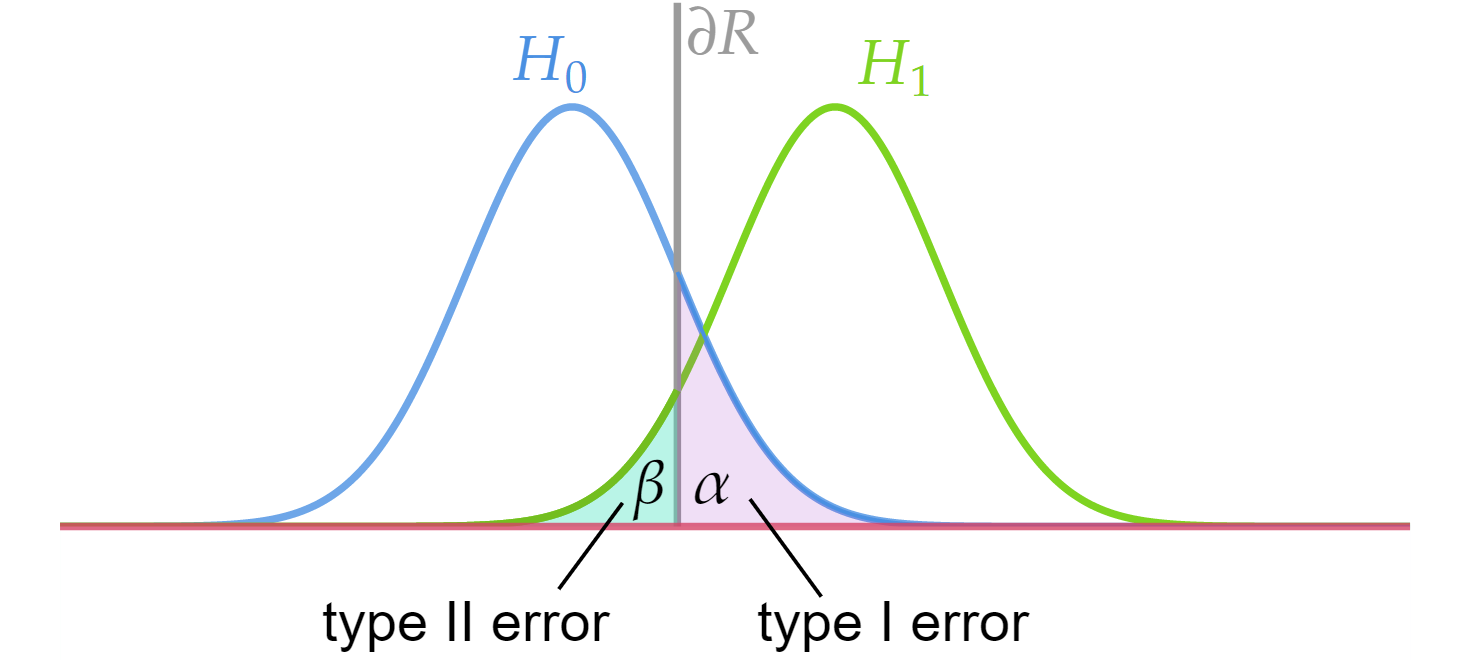
\includegraphics[width=0.55\linewidth]{sections/images/2022-09-05-16-16-51.png}
        \caption{Illustration of type I\&II error}
        \label{}
    \end{figure}
    

        
\begin{point}
        \textbf{Neyman-Pearson Principle}\index{Neyman-Pearson Principle}: First control $\alpha\leq\alpha_0$, then take $\min \beta$.
\end{point}


        How to determine $\alpha_0$? Depend on specific problem.\footnote{In most cases, take $\alpha_0=0.05$.}

        \item $p$-value: probability to get larger bias than observed $\vec{x}_0$ \uline{under $H_0$.}
        
        e.g. For reject region $R=\{\vec{X}|T(\vec{X})\geq C\},$ $p$-value:
        \begin{equation}
            p_{H_0}(\vec{x})=\mathbb{P}[T(\vec{X})\geq t(\vec{x}_0)|H_0]
        \end{equation}


        Remark: We believe that sample should reflect the property of model parameter, and $ p $-value is that under $H_0$, the probability to get a \textbf{worse} result than $\vec{x}$.
        
        Rule: Reject $H_0$ if $p(\vec{x}_0)\leq\alpha_0$.

        Note: $ p $-value is \textbf{different from} $ \alpha $ or type I error. $ p $-value is generated before we make decision while $ \alpha  $ arises after we decide how to make decisions. (But they do target the same result.)

        \item Power Function\index{Power Function}: (when $H_0$ is given), probability to reject $H_0$ by sampling.
        \begin{equation}
            \pi(\theta)=\begin{cases}
                \mathbb{P}(\text{type I error}),& \theta\in\Theta_0\\
                1-\mathbb{P}(\text{type II error}),& \theta\in\Theta_1
            \end{cases}
            =
            \begin{cases}
                \alpha(\theta),&\theta\in\Theta_0\\
                1-\beta(\theta),&\theta\in\Theta_1
            \end{cases}
        \end{equation}

        Express as test function:
        \begin{equation}
            \pi(\theta)=\mathbb{E}[\varphi(\vec{X})|\theta]
        \end{equation}

        A nice test: $\pi(\theta)$ small under $H_0$, large under $H_1$ (and grows very fast at the boundary of $ H_0 $ and $ H_1 $).
        \end{itemize}

        \begin{point}
            \textbf{General Steps of Hypothesis Testing:}
        \end{point}
        
        

        \begin{enumerate}[topsep=0pt]
            \item Propose $H_0\,\&\, H_1$.
            \item Determine $R$ (usually in the form of a statistic, e.g. $R=\{\vec{X}:T(\vec{X})\geq c\}$).
            \item Select a proper $\alpha$ (to determine $c$).
            \item Sampling, get sample (as well as $t(\vec{x})$), then 
            \begin{itemize}[topsep=-1pt,itemsep=-2pt]
                \item compare with $R$ and determine whether to reject/accept $H_0$, or
                \item calculate $ p $-value and determine whether to reject/accept$ H_0 $
            \end{itemize}
            
                
            

        \end{enumerate}

% \subsubsection{Hypotheses Testing for Common Distributions}
%     \begin{itemize}
%         \item Single normal distribution: $\vec{X}=(X_1,X_2,\ldots,X_n)$ i.i.d. from $N(\mu,\sigma^2)$
        
%         Testing $\mu$:


%     \end{itemize}

\subsubsection{Hypothesis Testing of Common Distributions}\label{SubSectionHypothesisTestingOfCommonDistributions}
    For some common distribution populations, determine rejection region $R$ under certain $H_0$ with confidence coefficient $\alpha$.

    Definition of necessary statistics see section {\autoref{SubSectionConfidenceIntervalForDistributions}}.

    \begin{enumerate}
        \item Single normal population:\index{t-test@$ t $-test}

        \begin{table}[H]
            \centering
            \renewcommand\arraystretch{1.2}
            \begin{tabularx}{\linewidth}{|c|c|c|Y|c|}
                \hline
                Condition&$H_0$&$H_1$&Testing Statistic $T$&Rejection Region $R$\\
                \hline
                \multirow{3}{*}{$\sigma^2$ known, test $\mu$}&$\mu=\mu_0$&$\mu\neq\mu_0$&\multirow{3}{*}{$T=\dfrac{\sqrt{n}(\bar{X}-\mu_0)}{\sigma}\sim N(0,1)$}&$|T|>N_\frac{\alpha}{2}$\\
                &$\mu\leq\mu_0$&$\mu>\mu_0$&&$T>N_\alpha$\\
                &$\mu\geq\mu_0$&$\mu<\mu_0$&&$T<-N_\alpha$\\
                \hline
                \multirow{3}{*}{$\sigma^2$ unknown, test $\mu$}&$\mu=\mu_0$&$\mu\neq\mu_0$&\multirow{3}{*}{$T=\dfrac{\sqrt{n}(\bar{X}-\mu_0)}{S}\sim t_{n-1}$}&$|T|>t_{n-1,\frac{\alpha}{2}}$\\
                &$\mu\leq\mu_0$&$\mu>\mu_0$&&$T>t_{n-1,\alpha}$\\
                &$\mu\geq\mu_0$&$\mu<\mu_0$&&$T<-t_{n-1,\alpha}$\\
                \hline
                \multirow{3}{*}{$\mu$ known, test $\sigma^2$}&$\sigma^2=\sigma_0^2$&$\sigma^2\neq\sigma_0^2$&\multirow{3}{*}{$T=\dfrac{nS_\mu^2}{\sigma_0^2}\sim \chi_n^2$}&$T<\chi^2_{n,1-\frac{\alpha}{2}}\cup T>\chi^2_{n,\frac{\alpha}{2}}$\\
                &$\sigma^2\leq\sigma_0^2$&$\sigma^2>\sigma_0^2$&&$T>\chi^2_{n,\alpha}$\\
                &$\sigma^2\geq\sigma_0^2$&$\sigma^2<\sigma_0^2$&&$T<\chi^2_{n,1-\alpha}$\\
                \hline
                \multirow{3}{*}{$\mu$ unknown, test $\sigma^2$}&$\sigma^2=\sigma_0^2$&$\sigma^2\neq\sigma_0^2$&\multirow{3}{*}{$T=\dfrac{(n-1)S^2}{\sigma_0^2}\sim \chi_{n-1}^2$}&$T<\chi^2_{n-1,1-\frac{\alpha}{2}}\cup T>\chi^2_{n-1,\frac{\alpha}{2}}$\\
                &$\sigma^2\leq\sigma_0^2$&$\sigma^2>\sigma_0^2$&&$T>\chi^2_{n-1,\alpha}$\\
                &$\sigma^2\geq\sigma_0^2$&$\sigma^2<\sigma_0^2$&&$T<\chi^2_{n-1,1-\alpha}$\\
                \hline
            \end{tabularx}
        \end{table}


    \item Double normal population:
    
    \begin{table}[htbp]
        \centering
        \renewcommand\arraystretch{1.2}
        \begin{tabularx}{\linewidth}{|c|c|c|Y|c|}
            \hline
            Condition&$H_0$&$H_1$&Testing Statistic $T$&Rejection Region $R$\\
            \hline
            \multirow{3}{*}{\makecell{$\sigma_1^2,\sigma_2^2$ known,\\test $\mu_1-\mu_2$}}&$\mu_1-\mu_2=\mu_0$&$\mu_1-\mu_2\neq\mu_0$&\multirow{3}{*}{$T=\dfrac{\bar{X}-\bar{Y}-\mu_0}{\sqrt{\dfrac{\sigma_1^2}{m}+\dfrac{\sigma_2^2}{n}}}\sim N(0,1)$}&$|T|>N_\frac{\alpha}{2}$\\
                &$\mu_1-\mu_2\leq\mu_0$&$\mu_1-\mu_2>\mu_0$&&$T>N_\alpha$\\
                &$\mu_1-\mu_2\geq\mu_0$&$\mu_1-\mu_2<\mu_0$&&$T<-N_\alpha$\\
                \hline
                \multirow{3}{*}{\makecell{$\sigma_1^2,\sigma_2^2$ unknown,\\test $\mu_1-\mu_2$}}&$\mu_1-\mu_2=\mu_0$&$\mu_1-\mu_2\neq\mu_0$&\multirow{3}{*}{\makecell{$T=\dfrac{\bar{X}-\bar{Y}-\mu_0}{S_\omega}\sqrt{\dfrac{mn}{m+n}}$\\$\sim t_{m+n-2}$}}&$|T|>t_{m+n-2,\frac{\alpha}{2}}$\\
                &$\mu_1-\mu_2\leq\mu_0$&$\mu_1-\mu_2>\mu_0$&&$T>t_{m+n-2,\alpha}$\\
                &$\mu_1-\mu_2\geq\mu_0$&$\mu_1-\mu_2<\mu_0$&&$T<-t_{m+n-2,\alpha}$\\
                \hline
                \multirow{3}{*}{\makecell{$\mu_1,\mu_2$ known,\\test $\dfrac{\sigma^2_1}{\sigma_2^2}$}}&$\sigma_1^2=\sigma_2^2$&$\sigma_1^2\neq\sigma_2^2$&\multirow{3}{*}{$T=\dfrac{S_{\mu_2}^2}{S_{\mu_1}^2}\sim F_{n,m}$}&\makecell{$T<F_{n,m,1-\frac{\alpha}{2}}$\\$\cup \,T>F_{n,m,\frac{\alpha}{2}}$}\\
                &$\sigma_1^2\geq\sigma_2^2$&$\sigma_1^2<\sigma_2^2$&&$T>F_{n,m,\alpha}$\\
                &$\sigma_1^2\leq\sigma_2^2$&$\sigma_1^2>\sigma_2^2$&&$T<F_{n,m,1-\alpha}$\\
                \hline
                \multirow{3}{*}{\makecell{$\mu_1,\mu_2$ unknown,\\test $\dfrac{\sigma^2_1}{\sigma_2^2}$}}&$\sigma_1^2=\sigma_2^2$&$\sigma_1^2\neq\sigma_2^2$&\multirow{3}{*}{$T=\dfrac{S_{2}^2}{S_{2}^2}\sim F_{n-1,m-1}$}&\makecell{$T<F_{n-1,m-1,1-\frac{\alpha}{2}}$\\$\cup\, T>F_{n-1,m-1,\frac{\alpha}{2}}$}\\
                &$\sigma_1^2\geq\sigma_2^2$&$\sigma_1^2<\sigma_2^2$&&$T>F_{n-1,m-1,\alpha}$\\
                &$\sigma_1^2\leq\sigma_2^2$&$\sigma_1^2>\sigma_2^2$&&$T<F_{n-1,m-1,1-\alpha}$\\
                \hline
        \end{tabularx}
    \end{table}

    \item None normal population:
    
    \begin{table}[htbp]
        \centering
        \renewcommand\arraystretch{1.7}
        \begin{tabularx}{\linewidth}{|c|c|c|Y|c|}
            \hline
            Condition&$H_0$&$H_1$&Testing Statistic $T$&Rejection Region $R$\\
            \hline
            \makecell{$\vec{X}$ from $B(1,p)$, test $p$}&$p=p_0$&$p\neq p_0$&$T=\dfrac{\sqrt{n}(\bar{X}-p_0)}{\sqrt{p_0(1-p_0)}}\xrightarrow[]{\mathscr{L}}N(0,1)$&$|T|>N_\frac{\alpha}{2}$\\
            \hline
            \makecell{$\vec{X}$ from $P(\lambda)$, test $\lambda$}&$\lambda=\lambda_0$&$\lambda\neq \lambda_0$&$T=\dfrac{\sqrt{n}(\bar{X}-\lambda_0)}{\sqrt{\lambda_0}}\xrightarrow[]{\mathscr{L}}N(0,1)$&$|T|>N_\frac{\alpha}{2}$\\
            \hline
        \end{tabularx}
    \end{table}
    \item More than two normal population: Analysis of Variance.
\end{enumerate}

\subsubsection{Likelihood Ratio Test}\label{SubSectionLRT}
    \index{LRT (Likelihood Ratio Test)}
    Idea: To test $H_0:\theta\in\Theta_0\longleftrightarrow H_1:\theta\in\Theta_1$ known $\vec{x}$, examine the likelihood function $L(\theta;\vec{x})$ and \textbf{compare} $L_{\theta\in\Theta_0}$ and $L_{\theta\in\Theta}$ to see the likelihood that $H_0$ is true.

    Def. \textbf{Likelihood Ratio} (LR):
    \begin{equation}
    \Lambda (\vec{x})=\dfrac{{\displaystyle\sup_{\theta\in\Theta_0}L(\theta;\vec{x})}}{{\displaystyle\sup_{\theta\in\Theta}L(\theta;\vec{x})}}
    \end{equation}

    Reject $H_0$ if $\Lambda(\vec{x})<\Lambda_0$. Or equivalently: Reject $H_0$ if $-2\ln\Lambda(\vec{x})>C(=-2\ln\Lambda_0)$.

    where $\Lambda_0$ (or equivalently $C=-2\ln\Lambda_0$) satisfies:
    \begin{equation}\mathbb{E}_{\Theta_0}[\varphi(\vec{X})]\leq\alpha,\quad\forall\theta\in\Theta_0\end{equation}

    LR and sufficient statistic: $\Lambda(\vec{x})$ can be expressed as $\Lambda(\vec{x})=\Lambda^*(T(\vec{x}))$, where $T(\vec{X})$ is sufficient statistic. We usually denote $ \lambda =\log \Lambda  $


\begin{point}
    LRT for one-sample $ t $-test: For $ X_1,X_2,\ldots,X_n $ i.i.d. $ \sim N(\mu,\sigma ^2) $, test

\[
    H_0: \mu=\mu_0\longleftrightarrow H_1:\mu\neq\mu_0\quad\text{when }\sigma ^2\text{ unknown}
\]

    Can prove:
    \[
        \lambda ^{2/n}=\dfrac{\sum\limits_{i=1}^n(x_i-\bar{x})^2}{\sum\limits_{i=1}^n(x_i-\mu_0)^2} 
    \]
    
    Denote $ T=\dfrac{\sqrt{n}(\bar{x}-\mu_0)}{S}$, then LRT could be expressed in equivalent form 
    \[
        \lambda  = \left( 1+\dfrac{T^2}{n-1} \right)^{-n/2}
    \]
    
    The Multivariate case see {\autoref{SubSectionMultivariateHypothesisTesting}}, where $ T^2 $ itself is the Hotelling's $ T^2 $ statistic.
    
    

\end{point}



\begin{point}
    Limiting Distribution of LRT: Wilks' Thm.\index{Wilk's Thm.}
\end{point}

    

    
    If $\dim\Theta=k>\dim\mathrm{span}\{\Theta_0\}=s$\footnote{Here 'dimension' refers to 'degree of freedom'.}, then under $H_0:\theta\in\Theta_0$:
    \begin{equation}
        -2\lambda =-2\ln \Lambda (\vec{x})\xrightarrow[]{\mathscr{L}}\chi_{k-s}^2
    \end{equation}

\subsubsection{Uniformly Most Powerful Test}\label{SUbSectionUMP}
    \index{UMPT (Uniformly Most Powerful Test)}Idea: Neyman-Pearson Principle: control $\alpha$, find $\min\beta$. i.e. control $\alpha$, find $\max\pi(\theta)$

    Def. \textbf{Uniformly Most Powerful Test} (UMP) $\varphi_{\mathrm{UMP}}$ with level of significance $\alpha$ satisfies
    \begin{equation}
        \pi_{\mathrm{UMP}}(\theta)\geq\pi(\theta),\,\forall\theta\in\Theta_1
    \end{equation}

    \textbf{Neyman-Pearson Lemma}\index{NP-Lemma (Neyman-Pearson Lemma)}: For $\vec{X}=(X_1,X_2,\ldots,X_n)$ i.i.d. from $f(\vec{x};\theta)$. 
    
    Test hypothesis $H_0:\theta=\theta_0\longleftrightarrow H_1:\theta=\theta_1$. Def. test function $\varphi$ as:
    \begin{equation}\label{UMPtestfunction}
        \varphi(\vec{x})=\begin{cases}
            1,&\dfrac{f(\vec{x};\theta_1)}{f(\vec{x};\theta_0)}>C\\
            r,&\dfrac{f(\vec{x};\theta_1)}{f(\vec{x};\theta_0)}=C\\
            0,&\dfrac{f(\vec{x};\theta_1)}{f(\vec{x};\theta_0)}<C
        \end{cases}
    \end{equation}

    Then there exists $C$ and $r$ such that
    \begin{itemize}
        \item $\mathbb{E}[\varphi(\vec{x})|\theta_0]=\mathbb{P}(\dfrac{f(\vec{x};\theta_1)}{f(\vec{x};\theta_0)}>C)+r\mathbb{P}(\dfrac{f(\vec{x};\theta_1)}{f(\vec{x};\theta_0)}=C)=\alpha$
        \item This $\varphi$ is UMP of level of significance $\alpha$
    \end{itemize}

    Actually kind of $1$-dimensional case of LRT.

    Note: UMT exist for\textbf{ simple }$H_0,H_1$, otherwise may not exist.

    UMP and sufficient statistics: Test function $\varphi(\vec{X})$ given by \autoref{UMPtestfunction} is function of sufficient statistics $T(\vec{X})$, i.e. $\varphi(\vec{X})=\varphi^*(T(\vec{X}))$.

    UMP and Exponential Family: For sample $\vec{X}=(X_1,X_2,\dots,X_n)$ from exponential family:
    \begin{equation}
    f(\vec{x};\theta)=C(\theta)h(\vec{x})\exp\{Q(\theta)T(\vec{x})\}    
    \end{equation}

    Test single hypothesis $H_0:\theta=\theta_0\longleftrightarrow H_1:\theta=\theta_1$, (where $ \theta_0<\theta_1 $ ).
    If 
    \begin{itemize}[topsep=0.5pt,itemsep=0pt]
        \item $\theta_0$ is inner point of $\Theta$
        \item $Q(\theta)$  monotone increase with $\theta$
    \end{itemize}

    Then UMP exists, in the form of:
    \begin{equation}\label{UMPtestfunctioninExponentialFamily}
            \varphi(\vec{x})=\begin{cases}
        1,&T(\vec{x})>C\\
        r,&T(\vec{x})=C\\
        0,&T(\vec{x})<C
    \end{cases} 
    \end{equation}
   
    

    where $C$ and $r$ satisfies $\mathbb{E}[\varphi(\vec{x})|\theta_0]=\alpha$.

    Note: or take $Q(\theta)$ mono decreased, then in \autoref{UMPtestfunctioninExponentialFamily}, take opposite inequality operators.
    
\begin{point}
    \textbf{General Steps of UMP}:
\end{point}

    
    \begin{enumerate}
        \item Find a point $\theta_0\in\Theta_0$ and a point $\theta_1\in\Theta_1$. (Note: \textbf{one} point)
        \item Construct test function in the form of {\autoref{UMPtestfunction}}, use $\mathbb{E}[\varphi(\vec{x})|\theta_0]=\alpha$ to determine $C$ and $r$.
        \item Get $R$ and $\varphi(\vec{x})$.
        \item If $\varphi$ does \textbf{not} depend on $\theta_1$, then $H_1$ can be generalized to $H_1:\theta\in\Theta_1$.
        \item If $\varphi$ satisfies $\mathbb{E}_{\theta\in\Theta_0}(\varphi)\leq\alpha$, then $H_0$ an be generalized to $H_0:\theta\in\Theta_0$.
    \end{enumerate}

\subsubsection{Duality of Hypothesis Testing and Interval Estimation}

\begin{itemize}
    \item Thm.: $\forall\theta_0\in\Theta$ there exists hypothesis testing $H_0:\theta=\theta_0\longleftrightarrow H_1:\theta\neq\theta_0$ of level $\alpha$ with rejection region $R_{\theta_0}$. Then
    \begin{equation}
        C(\vec{X})=\{\theta:\vec{X}\in R^C_{\theta}\}
    \end{equation}

    is a $1-\alpha$ confidence region for $\theta$

    \item Thm.: $C(\vec{X})$ is a $1-\alpha$ confidence region for $\theta$. Then $\forall\theta_0\in C(\vec{X})$, the rejection region of hypothesis testing $H_0:\theta=\theta_0\longleftrightarrow H_1:\theta\neq\theta_0$ of level $\alpha$ satisfies
    \begin{equation}
    R^\complement_{\theta_0}=\{\vec{X}:\theta_0\in C(\vec{X})\}
    \end{equation}
\end{itemize}
    
    \begin{point}
        Idea:
    \end{point}
    
        
\begin{itemize}[itemsep=-3pt]
    \item[] \centering $H_0:\theta=\theta_0\longleftrightarrow H_1:\theta\neq\theta_0$
    \begin{equation}\updownarrow\end{equation}
    \item[] \centering $\mathbb{P}(R^\complement(\vec{X})|H_0)=\mathbb{P}(R^\complement(\vec{X})|\theta_0)=1-\alpha$
    \begin{equation}\updownarrow\end{equation}
    \item[] Confidence Interval: $\theta_0\in R^\complement(\vec{X})$
\end{itemize}

    Similar for Confidence Limit and One-Sided Testing.

\subsubsection{Introduction to Non-Parametric Hypothesis Testing}\label{SubSectionIntroToNonParametricHypothesisTesting}

    Motivation: Usually distribution form unknown, cannot use parametric hypothesis testing.

    Useful Method:
    \begin{itemize}
        \item Sign Test: Used for paired comparison $\vec{X}=(X_1,X_2,\ldots,X_n)$, $\vec{Y}=(Y_1,Y_2,\ldots,Y_n)$.
        
        Take $Z_i=Y_i-X_i$ i.i.d., denote $E(Z)=\mu$. Test $H_0:\mu=0\longleftrightarrow H_1:\mu\neq 0$.

        Denote $n_+=\#(\text{positive } Z_i)$ and $n_-=\#(\text{negative }Z_i)$, $n_0=n_++n_-$. Then $n_+\sim B(n_0,\theta)$, test $H_0:\theta=\dfrac{1}{2}\longleftrightarrow H_1:\theta\neq\dfrac{1}{2}$
        
        Then use Binomial Testing or large sample CLT Normal Testing.

        Remark:
        \begin{itemize}
            \item Also can test $H_0:\theta\leq\dfrac{1}{2}\longleftrightarrow H_1:\theta>\dfrac{1}{2}$
            \item Drawback: ignores magnitudes.
        \end{itemize}
        
        \item \index{WSRT (Wilcoxon Signed Rank Sum Test)}Wilcoxon Signed Rank Sum Test: Improvement of Sign Test. Base on order statistics.
        
        Order Statistics of $Z_i$: $Z_{(1)}<Z_{(2)}<\ldots<Z_{(n)}$, where each $Z_{(j)}$ corresponds to some $Z_i$, denote as $Z_i=Z_{(R_i)}$, then $R_i$ is the rank of $Z_i$.\footnote{If some $X_i,X_j,\ldots$ equal, then take same rank $R=\mathrm{mean}\{R_i,R_j,\ldots\}$.}
        
        Def. $\vec{R}=(R_1,R_2,\ldots,R_n)$ is \textbf{Rank Statistics} of $(Z_1,Z_2,\ldots,Z_n)$

        Def. \textbf{Sum of Wilcoxon Signed Rank}: 
        \begin{equation}
        W^+=\sum_{i=1}^{n_0}R_i\mathbb{I}_{Z_i>0} 
        \end{equation}

        Distribution of $W^+$ is complex. $E$ and $var$ of $W^+$ under $H_0$:
        \begin{equation}
            \mathbb{E}(W^+)=\frac{n_0(n_0+1)}{4}\qquad var(W^+)=\frac{n_0(n_0+1)(2n_0+1)}{24}    
        \end{equation}

        Usually consider large sample CLT, construct normal approximation:
        \begin{equation}
            T=\frac{W^+-\mathbb{E}(W^+)}{\sqrt{var(W^+)}}\xrightarrow[]{\mathscr{L}}N(0,1)
        \end{equation}

        Rejection Region: $R=\{|T|>N_\frac{\alpha}{2}\}$

        \item Wilcoxon Two-Sample Rank Sum Test: Used for two independent sample comparison.\index{Wilcoxon Two-Sample Rank Sum Test}
        
        Assume $\vec{X}=(X_1,\ldots,X_m)$ i.i.d. $\sim f(x)$; $\vec{Y}=(Y_1,\ldots,Y_n)$ i.i.d. $\sim f(x-\theta)$, test $H_0:\theta=0\longleftrightarrow H_1:\theta\neq 0$.

        Rank $X_i$ and $Y_i$ as:
        \begin{equation}
            Z_1\leq Z_2\leq\ldots\leq Z_{m+n}
        \end{equation}

        in which denote rank of $Y_i$ as $R_i$, and def. \textbf{Wilcoxon two-sample rank sum}:
        \begin{equation}W=\sum_{i=1}^n R_i\end{equation}

        $\mathbb{E}$ and $var$ of $W$ under $H_0$:
\begin{equation}\mathbb{E}(W)=\frac{n(m+n+1)}{2}\qquad var(W)=\frac{mn(n+m+1)}{12}\end{equation}

        Use large sample approximation, construct CLT:
        \begin{equation}
            T=\frac{W-\mathbb{E}(W)}{\sqrt{var(W)}}\xrightarrow[]{\mathscr{L}}N(0,1)
        \end{equation}







        \item Goodness-of-Fit Test: For $\vec{X}=(X_1,X_2,\ldots,X_n)$ i.i.d. from some certain population $X$. Test $H_0:X\sim F(x)$.\index{Goodness-of-Fit Test}
        
        where $F$ is theoretical distribution, can be either parametric or non-parametric.

        Idea: Define some \textit{quantity} $D=D(X_1,\ldots,X_n;F)$ to measure the difference between $F$ and sample. And def. \textit{Goodness-of-fit} when observed value of $D$ (say $d_0$) is given:
        \begin{equation}p(d_0)=\mathbb{P}(D\geq d_0|H_0)\end{equation}

        \textbf{Goodness-of-Fit Test}: Reject $H_0$ if $p(d_0)<\alpha$.


            Pearson $\chi^2$ Test: Usually used for discrete case. 
            
            Test $H_0:\mathbb{P}(X_i=a_i)=p_i,\, i=1,2,\ldots,r$. Denote $\#(X_j=a_i)=\nu_i$, take $D$ as:
            \begin{equation}\label{Pearson_chi_test_differenceKn}
                K_n=K_n(X_1,\ldots,X_n;F)=\sum_{i=1}^r\frac{(\nu_i-np_i)^2}{np_i}
            \end{equation}

            Pearson Thm.: For $K_n$ defined as \autoref{Pearson_chi_test_differenceKn}, then under $H_0$:
            \begin{equation}
                K_n\xrightarrow[]{\mathscr{L}}\chi^2_{r-1-s}
            \end{equation} 

            Here $s$ is number of unknown parameter, $r-1-s$ is the degree of freedom.

            Note:
            \begin{itemize}
                \item $a_i$ must \textbf{not} depend on sample.
                \item For continuous case, construct division:
                \begin{equation}\mathbb{R}\rightarrow(-\infty,a_1,a_2,\ldots,a_{r-1},\infty=a_r) \end{equation}

                and test $H_0:\mathbb{P}(X\in I_j)=p_j$

                Criterion: Pick proper interval so that $np_i$ and $\nu_i$ both $\geq 5$.
            \end{itemize}
 


        \item Contingency Table Independence \& Homogeneity Test
        \index{Contingency Table}
 
\begin{itemize}
    \item Independence Test:\index{Pearson's $ \chi^2 $ Test}
    
    Test a two-parameter sample and to see whether these two parameters(features) are independent. Denote $Z=(X,Y)$ are some 'level' of sample, $n_{ij}$ is number of sample with level $(i,j)$

    Contingency Table:
    \begin{table}[H]
        \centering
        \begin{tabular}{|c|ccccc|c|}
            \hline
            \diagbox{X}{Y}&1&$\ldots$&$j$&$\ldots$&$s$&$\sum$\\
            \hline
            1&$n_{11}$&$\ldots$&$n_{1j}$&$\ldots$&$n_{1s}$&$n_{1\cdot}$\\
            $\vdots$&$\vdots$&$\ddots$&$\vdots$&$\ddots$&$\vdots$&$\vdots$\\
            $i$&$n_{i1}$&$\ldots$&$n_{ij}$&$\ldots$&$n_{is}$&$n_{i\cdot}$\\
            $\vdots$&$\vdots$&$\ddots$&$\vdots$&$\ddots$&$\vdots$&$\vdots$\\
            $r$&$n_{r1}$&$\ldots$&$n_{rj}$&$\ldots$&$n_{rs}$&$n_{r\cdot}$\\
            \hline
            $\sum$&$n_{\cdot 1}$&$\ldots$&$n_{\cdot j}$&$\ldots$&$n_{\cdot s}$&$n$\\
            \hline
        \end{tabular}
    \end{table}

        Test $H_0:X\,\&\, Y$ are independent. i.e. $H_0:P(X=i,Y=j)=P(X=i)P(Y=j)=p_{i\cdot}p_{\cdot j}$.

        Construct $\chi^2$ test statistic:
        \begin{equation}
            K_n=\sum_{i=1}^r\sum_{j=1}^s\frac{[n_{ij}-n(\frac{n_{i\cdot}}{n})(\frac{n_{\cdot j}}{n})]^2}{n(\frac{n_{i\cdot}}{n})(\frac{n_{\cdot j}}{n})}=n\left(\sum_{i=1}^r\sum_{j=1}^s\frac{n_{ij}^2}{n_{i\cdot}n_{\cdot j}}-1\right)
        \end{equation}

        Then under $H_0$, $K_n\xrightarrow[]{\mathscr{L}}\chi^2_{rs-1-(r+s-2)}=\chi^2_{(r-1)(s-1)}$

        Reject $H_0$ if $p(k_0)=P(K_n\geq k_0)<\alpha$


        \item Homogeneity Test:
        
        Test $R$ groups of sample with category rank, to see whether these groups has similar rank distribution.

        \begin{table}[H]
            \centering
            \begin{tabular}{|c|ccccc|c|}
                \hline
                \diagbox{Group}{Category}&Category 1&$\ldots$&Category $j$&$\ldots$&Category $C$&$\sum$\\
                \hline
                Group 1&$n_{11}$&$\ldots$&$n_{1j}$&$\ldots$&$n_{1C}$&$n_{1\cdot}$\\
                $\vdots$&$\vdots$&$\ddots$&$\vdots$&$\ddots$&$\vdots$&$\vdots$\\
                Group $i$&$n_{i1}$&$\ldots$&$n_{ij}$&$\ldots$&$n_{iC}$&$n_{i\cdot}$\\
                $\vdots$&$\vdots$&$\ddots$&$\vdots$&$\ddots$&$\vdots$&$\vdots$\\
                Group $R$&$n_{R1}$&$\ldots$&$n_{Rj}$&$\ldots$&$n_{RC}$&$n_{R\cdot}$\\
                \hline
                $\sum$&$n_{\cdot 1}$&$\ldots$&$n_{\cdot j}$&$\ldots$&$n_{\cdot C}$&$n$\\
                \hline
            \end{tabular}
        \end{table}


    Denote $P(\text{Category }j|\text{Group }i)=p_{ij}$. Test $H_0:p_{ij}=p_j,\,\forall 1\leq i\leq R$.

    Construct $\chi^2$ test statistic:
    \begin{equation}
        D=\sum_{i=1}^R\sum_{j=1}^C\frac{[n_{ij}-n(\frac{n_{i\cdot}}{n})(\frac{n_{\cdot j}}{n})]^2}{n(\frac{n_{i\cdot}}{n})(\frac{n_{\cdot j}}{n})}=n\left(\sum_{i=1}^R\sum_{j=1}^C\frac{n_{ij}^2}{n_{i\cdot}n_{\cdot j}}-1\right)
    \end{equation}

    Then under $H_0$, $D\xrightarrow[]{\mathscr{L}}\chi^2_{R(C-1)-(C-1)}=\chi^2_{(R-1)(C-1)}$
    \end{itemize}

    \item \hypertarget{testofnormality}{Test of Normality}: normality is a good \& useful assumption.
    
    For $\vec{Y}=(Y_1,Y_2,\ldots,Y_n)$,

    Test $H_0:\text{exists }\mu\,\&\, \sigma^2$ such that $Y_i$ i.i.d. $\sim N(\mu,\sigma^2)$.

    \begin{itemize}
        \item Kolmogorov-Smirnov Test\index{K-S Test (Kolmogorov-Smirnov Test)}: Assume $\vec{X}$ form population CDF $F(x)$, test $H_0:F(x)=F_0(x)$(where can take $F_0=\Phi$ or some other known CDF).
        
        use $F_n(x)$ (as defined in \autoref{empiricaldisreibutionfunction}) as approx. to $F(x)$, test
        \begin{equation}
            D_n=\sum_{-\infty< x<+\infty}|F_n(x)-F_0(x)|
        \end{equation}

        Reject $H_0$ if $D_n>c$

        or use goodness-of-fit: denote observed value of $D_n$ as $d_n$. Reject $H_0$ if
        \begin{equation}
            p(d_n)=\mathbb{P}(D_n>d_n|H_0)<\alpha
        \end{equation}

        \item Shapiro-Wilk Test:\index{S-W Test (Shapiro-Wilk Test)}
        
        Test $H_0:\text{exists }\mu\,\&\, \sigma^2$ such that $X_i$ i.i.d. $\sim N(\mu,\sigma^2)$.

        Denote $Y_{(i)}=\dfrac{X_{(i)}-\mu}{\sigma}$, $m_i=\mathbb{E}(Y_{(i)})$

        Under $H_0$, $(X_{(i)},m_i)$ falls close to straight line. Test Statistic: Correlation
        \begin{equation}
            R^2=\dfrac{\left(\sum_{i=1}^n(X_{(i)}-\bar{X})(m_i-\bar{m})\right)^2}{\sum_{i=1}^n(X_{i}-\bar{X})^2\sum_{i=1}^n(m_i-\bar{m})^2}=corr(X_{(i)},m_i)
        \end{equation}

        Reject $H_0$ if $R^2<c$

        Shapiro-Wilk correction:
        \begin{equation}
            W=\dfrac{\left(\sum_{i=1}^{[n/2]}a_i(X_{(n+1-i)}-X_{(i)})\right)^2}{\sum_{i=1}^n(X_{(i)}-\bar{X})^2}
        \end{equation}
    \end{itemize}
\end{itemize}

\begin{point}
    Summary: Useful Non-Parameter Hypothesis Testing.
\end{point}
\\
\\

\begin{equation*}
    \text{\makecell{Non-Parameter\\Hypothesis Testing}}
    \smash[htbp]{
    \begin{cases}
        \text{One Population Sample}
            \smash[t]{
                \begin{cases}
                    \chi^2\text{ Test}\\
                    \text{Binomial Test}\\
                    \text{One-Sample K-S Test}\\
                    \text{Wilcoxon Sign Test}\\
                    \text{Runs Test}
                \end{cases}
            }\\
            \\
            \\
            \\
            \\
        \text{Two Population Sample}
            \smash[t]{
                \begin{cases}
                    \text{Independent Sample}
                    \smash[t]{
                        \begin{cases}
                            \text{Mann-Whitney Test}\\
                            \text{K-S Test}\\
                            \text{Wald-Wolfowitz Test}\\
                            \text{Moses Test of Extreme Reactions}
                        \end{cases}
                    }\\
                    \\
                    \text{Relative Sample}
                    \smash[b]{
                        \begin{cases}
                            \text{Sign Test}\\
                            \text{McNemar Test}\\
                            \text{Wilcoxon Rank Sum Test}\\
                            \text{Marginal Homogeneity Test}
                        \end{cases}
                    }
                \end{cases}
            }\\
            \\
            \\
            \\
        \text{Multi-Population Sample}
            \smash[b]{
                \begin{cases}
                    \text{Independent Sample}
                    \smash[t]{
                        \begin{cases}
                            \text{Median Test}\\
                            \text{K-W One-Way ANOVA Test}\\
                            \text{Jonckheere-Terpstra Test}
                        \end{cases}
                    }\\
                    \\
                    \text{Relative Sample}
                    \smash[b]{
                        \begin{cases}
                            \text{Friedman Rank Sum Test}\\
                            \text{Kendall's Coefficient of Concordance Test}\\
                            \text{Cochran Q Test}
                        \end{cases}
                    }
                \end{cases}
            }
    \end{cases}  
    }
\end{equation*}

\newpage

 \section{R语言命令部分}
%     This part base on R x64 4.0.3 on VSCode 1.52.1

% \subsection{Basic}

\subsection{Basic Command}

\begin{table}[htbp]
    \centering
    \renewcommand\arraystretch{0.9}
    \begin{tabular}{l|l}
        \hline
        Action$\qquad\qquad\qquad\qquad\qquad\qquad\qquad$&Command$\qquad\qquad\qquad\qquad\qquad$\\
        \hline
        Get help&Hover on function name\\
        Get \textbf{example}&\lstinline|example('')|\\
        \textbf{Get} current \textbf{w}orking \textbf{d}irectory&\lstinline|getwd()|\\
        \textbf{L}i\textbf{s}t all objects&\lstinline|ls()|\\
        \textbf{R}e\textbf{m}ove objects&\lstinline|rm()|\\
        Remove all objects&\lstinline|rm(list <- ls())|\\
        Install package&\lstinline|install.packages('')|\\
        Load package&\lstinline|library('')|\\
        \hline
    \end{tabular}
\end{table}

% \subsubsection{Data Structures}
% \begin{itemize}[topsep=6pt,itemsep=4pt]
%     \item Vector: One-dimensional array
    
%     \begin{point}
%         Def. a vector
%     \end{point}
% \begin{lstlisting}[language=R]
%     myvector <- c(elements)
% \end{lstlisting}

%     Note: here \lstinline|c()| for '\textbf{c}ombine'.
    
%     \begin{point}
%         Index reference
%     \end{point}
    
% \begin{lstlisting}[language=R]
%     myvector[3]
%     myvector[c(2,4)]
%     myvector[2:4]
% \end{lstlisting}
    
%     \item Matrix: Two-dimensional array
%     \begin{point}
%         Def. a matrix
%     \end{point}
% \begin{lstlisting}[language=R]
%     mymatrix <- matrix(vector, nrow, ncol, byrow, dimname)
% \end{lstlisting}

% \begin{point}
%     Index reference
% \end{point}
% \begin{lstlisting}[language=R]
%     mymatrix[2,4]
% \end{lstlisting}


%     \item Array
%     \item \textbf{Data.Frame} 
%     \item List 
% \end{itemize}

    



% \subsection{Statistics Method}




% \subsection{Graph}



\subsection{Useful Packages}

\subsubsection{\consolas{ggplot2} package}
    \lstinline|ggplot2| for `the \textbf{G}rammar of \textbf{G}raphics \textbf{Plot}' (\textbf{2}$^\mathrm{nd}$ version). \\
    Key thought: separate statistics operation (\lstinline|stat_|) and geometric operation (\lstinline|geom_|) and other parts.

    Basic syntax structures for a \lstinline|ggplot2| figure:
\begin{lstlisting}[language=R]
ggplot(data = , aes(x = , y = , ...)) +
    geom_XXX(...) + stat_XXX(...) + ... +
    annotate(...)+ ... +
    scale_XXX(...) + coord_XXX(...) + guides(...) + theme(...)    
\end{lstlisting}


\begin{itemize}[topsep=6pt,itemsep=4pt]
    \item 
\end{itemize}

    
\begin{point}
    \lstinline|aes()| for `aesthetic': Describe how variables in the data are mapped to visual properties (aesthetics) of \lstinline|geom| layer.
\end{point}



    \lstinline|geom_| functions describes
\begin{table}[H]
    \centering
      \begin{tabular}{l|l|l}
        \hline
      Functions  & Adds  & Options \\
      \hline
      \lstinline|geom_bar()|  & Bar chart  & \lstinline|color; fill; alpha | \\
      \lstinline|geom_boxplot()|  & Box plot  & \lstinline|color; fill; alpha; notch; width | \\
      \lstinline|geom_density()|  & Density plot  & \lstinline|color; fill; alpha; linetype | \\
      \lstinline|geom_histogram()|  & Histogram  & \lstinline|color; fill; alpha; linetype; binwidth | \\
      \lstinline|geom_hline()|  & Horizontal lines  & \lstinline|color; alpha; linetype; size | \\
      \lstinline|geom_jitter()|  & Jittered points  & \lstinline|color; size; alpha; shape | \\
      \lstinline|geom_line()|  & Line graph  & \lstinline|colorvalpha; linetype; size | \\
      \lstinline|geom_point()|  & Scatterplot  & \lstinline|color; alpha; shape; size | \\
      \lstinline|geom_rug()|  & Rug plot  & \lstinline|color; side | \\
      \lstinline|geom_violin()|  & Violin plot  & \lstinline|color; fill; alpha; linetype | \\
      \lstinline|geom_vline()|  & Vertical lines  & \lstinline|color; alpha; linetype; size | \\
      \hline
      \lstinline|geom_smooth()|  & Fitted line  & \lstinline|method; formula; color; fill; linetype; size | \\
      \lstinline|geom_text()|  & Text annotations & See the help for this function \\
      \hline
      \end{tabular}
  \end{table}
  
  Some useful \lstinline|geom_| function options (More options see `R in Action P445'):
\begin{table}[H]
    \centering
    \renewcommand\arraystretch{1}
    \begin{tabular}{l|l}
        \hline
        Options&Specifies\\\hline
        \lstinline|color|&Color of points\&lines\&borders of regions.\\
        \lstinline|fill|&Color of filled areas.\\
        \lstinline|alpha|&Transparency (0-1)\\
        \lstinline|linetype|&Line pattern see table.\\%%%%
        \lstinline|size|&Size of points\&lines.\\
        \lstinline|shape|&Point shape see table.\\%%%%%
        \lstinline|width|&Width of box plots.\\
        \lstinline|position|&\lstinline|dodge|/\lstinline|stack|/\lstinline|jitter| etc. position relation.\\
        \hline
        \lstinline|method|&Smoothing function to use.\\
        \lstinline|formula|&Smoothing formula, e.g. \lstinline|y~log(x)|.\\
        \lstinline|se|&Confidence interval (\lstinline|TRUE|/\lstinline|FALSE|).\\
        \lstinline|level|&Level of confidence interval.\\
    \end{tabular}
\end{table}



\lstinline|facet_| trellis command.
\begin{table}[H]
    \centering
    \renewcommand\arraystretch{1}
    \begin{tabular}{l|l}
        \hline
        \lstinline|facet_warp(~var,ncol)|&Separate plots by column.\\
        \lstinline|facet_warp(~var,nrow)|&Sparate plots by row.\\
        \lstinline|facet_grid(rowvar~colvar)|&Separate plots into combination of \lstinline|rowvar| and \lstinline|colvar|.\\
        \lstinline|facet_grid(row|&\\

        \hline
    \end{tabular}
\end{table}





\subsubsection{\consolas{data.frame} and \consolas{dplyr} package}


 \newpage

\section{线性回归分析部分}\label{SecLinearRegressionAnalysis}
\begin{point}
    Steps in Regression Analysis
\end{point}

\begin{enumerate}[topsep=2pt,itemsep=2pt]
    \item Exploratory Data Analysis (EDA)\index{EDA (Exploratory Data Analysis)}
    \item Statement of the problem;
    \item Selection of potentially relevant variables;
    \item Data collection;
    \item Model specification;
    \item Choice of fitting method;
    \item Model fitting;
    \item Model validation and criticism;
    \item Using the chosen model(s) for the solution of the posed problem.
\end{enumerate}

    

\subsection{Linear Regression Model}
\begin{itemize}[topsep=6pt,itemsep=4pt]
    \item Assume a Model
    \begin{enumerate}[topsep=6pt,itemsep=4pt]
        \item Parameter of the model
        \item Basic Assumptions
        \item Dsitribution of error
    \end{enumerate}
    \item Parametric Estimation
    \begin{enumerate}[topsep=6pt,itemsep=4pt]
        \item Ordinary Least Squares Estimation
        \item Maximun Likelihood Estimation
    \end{enumerate}
    \item Statistics Inference
    \begin{enumerate}[topsep=6pt,itemsep=4pt]
        \item Hypotheses Testing
        \item Interval Estimation
    \end{enumerate}

\end{itemize}


    


        
\subsubsection{Data for simple linear regression}

    We will observe pairs of variables, called 'cases'(样本点)
        
    A sample is $ (X_1,Y_1),\ldots,(X_n,Y_n) $

    Linear Model: \footnote{Here in linear regression, we consider $ X_i $ only as real number, \textbf{without} randomness. So here $ Y_i $ can be considered as an r.v. with $ X_i $ as parameter, i.e. $ Y_i|_{X_i=x_i} $}

%% 关于线性模型的X_i性质的假定
    \[
        Y_i=\beta _0+\beta _1X_i+\varepsilon _i 
    \]
    where $ \varepsilon_i  $ i.i.d.$ \sim \varepsilon  $ is a random error term, satisfies    \footnote{Note: Why we need $ \varepsilon $ as 'random error term'?
    \begin{itemize}[topsep=6pt,itemsep=4pt]
        \item It represents the intrinsic random property of the model.
        \item Based on $ \varepsilon  $, we can take r.v. into our statistic model.
    \end{itemize}
    }
    
    \[
        E(\varepsilon _i)=0\qquad var(\varepsilon _i)=\sigma ^2 
    \]
    
    

    Normal Error Assumption: Further in most cases, we consider $ \varepsilon \sim N(0,\sigma^2) $ ----because of its well-property distribution, $ \varepsilon _1,\varepsilon _2,\ldots,\varepsilon _n $ i.i.d. $ N(0,\sigma ^2) $.\footnote{i.e. $ Y_i $ are independent
    \[
        Y_i\sim N(\beta _0+\beta _1X_i,\sigma^2)\quad i=1,2,\ldots ,n 
    \]
    
    }
        
    What does Linear Regression do? Under Linear Model, try to estimate 
    \begin{itemize}[topsep=0pt,itemsep=-2pt]
        \item $ \beta _0\text{ (intercept) }$;
        \item $\beta _1\text{ (slope) }$;
        \item $\sigma ^2\text{ (variance of error)} $.
    \end{itemize}
    
    
    (Thus Linear Regression is also a Statistics Inference process: deduce properties of model from data)
        
\subsubsection{The Ordinary Least Square Estimation}
    Aim: use $ (x_i,y_i) $  to estimate $ \beta _0,\beta _1,\sigma^2 $. The idea is to define a 'loss function' to reflect the 'distance' from sample point to estimation point.

    Estimate Principle: \footnote{Detailed Definition and Derivation see sec.\ref{SubSectionMoM_MLE_LinearRegression}.}
    \begin{itemize}[topsep=2pt,itemsep=2pt]
        \item Ordinary Least Squares\index{Ordinary Least Squares}:
        \[
            (\hat{\beta  }_0,\hat{\beta _1})=\arg\min\sum_{i=1}^n (y-\beta _0-\beta _1x_i)^2
        \]
        \item MLE or MoM Estimation.
    \end{itemize}
    

    
    And get $ \hat{\beta _1},\hat{\beta _0}$ as well as $ \hat{\sigma^2} $(see eqa(\ref{EqaOLSEstimatorOfSigma}):\footnote{A memory trick: use $ \dfrac{Y}{\sqrt{s_Y}}=r_{XY}\dfrac{X}{\sqrt{s_X}} $ to get formular of $ Y\sim X $:
    \[
        \hat{\beta }_1=r_{XY}\dfrac{\sqrt{s_Y}}{\sqrt{s_X}}=\dfrac{{\displaystyle\sum (x_i-\bar{x})(y_i-\bar{y})}}{{\displaystyle\sum (x_i-\bar{x})^2}} 
    \]}

%LSE beta_0 beta_1
\begin{equation}\label{EqaOLSEstimatorOfBeta}
    \begin{aligned}
        \hat{\beta }_1=&\dfrac{\sum\limits_{i=1}^n (x_i-\bar{x})(y_i-\bar{y})}{\sum\limits_{i=1}^n (x_i-\bar{x})^2}\\
        \hat{\beta }_0=&\bar{y}-\hat{\beta _1}\bar{x}\\
        \hat{\sigma^2}=&\dfrac{1}{n-p-1}\sum_{i=1}^n(y_i-\hat{\beta }_0-\hat{\beta }_1x_i)^2
    \end{aligned}
\end{equation}


    
    Def. \index{Residual}\textbf{Residual}: distance from sample point to estimate point, to reflect how the sample points fit the model.
    \[
        e_i=y_i-\hat{y}_i=\text{observed value of }\varepsilon _i 
    \]
    
    Note: under least square estimation, we have\footnote{Intuitively, they each means '$ E(\varepsilon )=0 $' and '$ X\parallel \varepsilon  $'.}
\begin{equation}\label{Limit_to_Residual}
        \sum e_i=0\qquad \sum x_ie_i=0 
\end{equation}
    

    Then use $ e_i $ to estimate $ \sigma ^2 $ (because it is $ \varepsilon _0 $ that are i.i.d., not $ Y_i $), where $ (n-p-1) $ is Degree of Freedom (df or dof)\footnote{Generally, MLE and LSE are different.

    Comment from R.A.Fisher: $ \sum e_i^2 $ should be divided by 'number of $ e_i^2 $ that contribute to variance'. Here $ (n-p-1) $ corresponds to 'degree of freedom' $ =(n-2) $, $ p=1 $ corresponds to `one' variable (see sec.\ref{SubSectionMoM_MLE_LinearRegression}, eqa(\ref{EqaEstimatorSigmaWithDoF})), and correponds to the two equations of $ e_i $, eqa(\ref{Limit_to_Residual})}
\begin{equation}\label{EqaOLSEstimatorOfSigma}
    \begin{aligned}
        \hat{\sigma _n^2}&=\dfrac{1}{n}\sum e_i^2 \quad\text{(use MLE or MoM)}\\
        \hat{\sigma^2}&=\dfrac{1}{n-p-1}\sum e_i^2=\dfrac{1}{n-2}\sum e_i^2\quad\text{(use OLS, unbiased)}
\end{aligned}
\end{equation}

    % MSE SSE dof






    % Review: Statistical Inference
    % \begin{itemize}[topsep=6pt,itemsep=4pt]
    %     \item Basic concepts: HT CI;
    %     \item Inference about $ \beta _1$;
    %     \item Inference about $ \beta _0 $.
    % \end{itemize}

    % Note: the distribution of $ \hat{\beta }_0,\hat{\beta }_1 $ is sampling distribution(抽样分布): distribution of statistics.



    % Power function of testing
    % \begin{itemize}[topsep=6pt,itemsep=4pt]
    %     \item Definition;
    %     \item Calculation;
    %     \item Sample<->Power (Calculation of sampling).
    % \end{itemize}


\subsubsection{Statistical Inference to $ \beta _0 $,$ \beta _1 $}

\begin{point}
    Sampling Distribution of $ \hat{\beta} _1,\hat{\beta} _0  $
\end{point}

    Consider $ \hat{\beta} _1,\hat{\beta} _0 $ as statistics of sample, then we can examine the sampling distribution of $  \hat{\beta} _1,\hat{\beta} _0 $. Their randomness comes from
    \[
        Y_i=\beta_0+\beta_1X_i+\varepsilon _i 
    \]
    
    

    (The following part treats $\hat{\beta} _1,\hat{\beta} _0 $ as r.v., and note that $ X_i $ are \textbf{not }r.v.. And  for convenience and conciseness, denote $ S_{XX}={\displaystyle\sum_{i=1}^n(X_i-\bar{X})^2} $)

   
\begin{align*}
        \hat{\beta }_1&=\beta _1+\sum_{i=1}^n\dfrac{X_i-\bar{X}}{S_{XX}}\varepsilon _i\\
        \hat{\beta }_0&=\beta _0+\sum_{i=1}^n\left(\dfrac{1}{n}-\dfrac{(X_i-\bar{X})\bar{X}}{S_{XX}}\right)\varepsilon _i
\end{align*}
 
    Denote corresponding variance as $ \sigma^2_{\hat{\beta}_1} $ and $ \sigma^2_{\hat{\beta}_0} $, using eqa(\ref{EqaDistributionOfSumOfiidNormal}) to get:
    \[
        \sigma^2_{\hat{\beta}_1}= \dfrac{\sigma^2}{S_{XX}}\qquad \sigma^2_{\hat{\beta}_0}=\sigma^2(\dfrac{1}{n}+\dfrac{\bar{X}^2}{S_{XX}})
    \] 
    
     And under normal error assumption, distribution of $ \hat{\beta} _1,\hat{\beta} _0  $ are
    \begin{align*}
        \hat{\beta }_1&\sim N(\beta _1,\sigma^2_{\hat{\beta}_1}) =N(\beta_1,\dfrac{\sigma^2}{S_{XX}})\\
        \hat{\beta}_0&\sim N(\beta_0,\sigma^2_{\hat{\beta }_0}) =N(\beta_0,\sigma^2(\dfrac{1}{n}+\dfrac{\bar{X}^2}{S_{XX}}))
    \end{align*}
    
    Based on sampling distribution of $ \hat{\beta} _1,\hat{\beta} _0  $, we can conduct statistical inference, including CI and HT.\footnote{Detail see sec.\ref{SectionHypothesisTesting}, estimating/testing $ \hat{\beta} _1,\hat{\beta} _0  $ usually corresponds to 'estimate $ \mu $, with $ \sigma^2 $ unknown'.}
    
    % \begin{itemize}[topsep=2pt,itemsep=2pt]
    %     \item LSE of $ \beta _1 $ gives 
    %     \[
    %         \hat{\beta _1}=\dfrac{\sum (x_i-\bar{x})(y_i-\bar{y})}{\sum (x_i-\bar{x})^2}
    %     \]
        
    %     and satisfies $ E(\hat{\beta}_1)=\beta_1 $. Can prove that $ \hat{\beta }_1\sim N(\beta _1,\dfrac{\sigma ^2}{\sum (x_i-\bar{x})^2})=N(\beta_1,\sigma^2(\hat{\beta}_1))$
       
    % \end{itemize}
    
    Note: In linear regression model, we usually focus more on $ \beta_1 $. And note that when $ 0 $ is \textbf{not} within the fitting range,$ \beta_0 $ is not so important.\footnote{Two reason:\begin{itemize}[topsep=2pt,itemsep=2pt]
        \item The etimation error of $ Y $ from $ \hat{\beta}_1 $ increases with $ X_h-\bar{X} $;
        \item $ \beta_1==0  $ is important: decides whether linear model can be used. 
    \end{itemize}
    
        }

    Why we choose OLS to get regression coefficients?

\begin{point}
    \index{Gauss-Markov Thm.`'}Gauss–Markov Thm.: the OLS estimator has the lowest sampling variance within the class of linear unbiased estimators, i.e. OLS is the Best Linear Unbiased Estimator(BLUE).\footnote{This Thm. does \textbf{not }require normal error assumption.}
\end{point}
    



\subsubsection{Prediction to $ Y_h $}
    For a new $ X_h $ at which we wish to \textbf{predict }the corresponding $ Y_h $ (based on other known point $ (X_i,Y_i) $), denote the estimator as $ \hat{\mu}_h $:
    \[
        \hat{\mu}_h=\hat{\beta}_1X_h+\hat{\beta}_0 =\beta_1X_h+\beta _0+\sum_{i=1}^n\left( \dfrac{1}{n}+\dfrac{(X_i-\bar{X})(X_h-\bar{X})}{S_{XX}} \right)\varepsilon _i
    \]
    
    Thus we can get\footnote{So $ \sigma ^2(\hat{\mu }_h) $ increases with $ X_h-\bar{X} $. Intuitively it make sense, because $ (\bar{X},\bar{Y})$ must falls on regression line.}
    \[
        E(\hat{\mu}_h)= \beta _1X_h+\beta _0\qquad \sigma ^2_{\hat{\mu}_h}=\left( \dfrac{1}{n}+\dfrac{(X_h-\bar{X})^2}{S_{XX}} \right)\sigma^2
    \]
    
    Under Normal assumption:
    \[
        \hat{\mu}_h\sim N(\beta _1X_h+\beta _0,\left( \dfrac{1}{n}+\dfrac{(X_h-\bar{X})^2}{S_{XX}} \right)\sigma^2) 
    \]
    
    Base on distribution we can give CI and HT.

    Note: Remember that when we consider the estimator $ \hat{\mu } $, we \textbf{must } have the randomness of $ \hat{\beta }_0,\hat{\beta }_1 $ considered(if they are unknown).
    
    Prediction Error: $ Y_h $ itself is an $ Y $ of the linear model, i.e. $ Y_i=\beta_0+\beta_1X_h+\varepsilon _h $, we can consider \textbf{$ Y_h $ itself as an r.v. }v.s.\textbf{ predicted $ Y_h $ from other sample points} and define \textbf{Prediction Error}: 
    \[
        d_h=Y_h-\hat{\mu}_h 
    \]

    
    \[
        E(d_h)=0\qquad \sigma^2_{d_h}=var(Y_h-\hat{\mu }_h)=\sigma^2\left[ 1+\dfrac{1}{n}+\dfrac{(X_h-\bar{X})}{S_{XX}} \right] > \sigma ^2_{\hat{\mu}_h}
    \]
    


    \begin{point}
       Simultaneous Confidence Band(SCB)\index{SCB (Simultaneous Confidence Band)}\index{CB (Confidence Band)}
    \end{point}

    Confidence Band is \textbf{not} the CI at each point, but really a \textbf{band} for the \textbf{entire} regression line.\footnote{Why they are different? We require the confidence band have a \textbf{simultaneous} converage probability. For the same band $ (L(x),U(x)) $, $ P(\text{the whole line})< P(\text{each point})$, so Confidence Band is wider than $ \bigcup $CIs to hold the same $ 1-\alpha $.
    
    Also, we will see that for linear model, the boundary of SCB forms hyperbola, which make sense considering its asymptotic line.}
    
    
    Aim: Find lower and upper function $ L(x) $ and $ U(x) $ such that
    \[
        P[L(x)<(\beta _0+\beta _1x)<U(x),\,\forall x\in I_x]=1-\alpha  
    \]
    
    and get \textbf{Confidence Band}:
    \[
        \{(x,y)|L(x)<y<U(x)|\forall x\in I_x\} 
    \]
    
    % Note: \textbf{Cannot} use CI at each point to form Confidence Band. Band is wider. And we are actually conduce CI \textbf{simoutanesly} to all $ x $.

    Where $ (L(x),U(x)) $ can be derived as
    \[
        (L(x),U(x))=\hat{\mu}_x\pm s_{\hat{\mu}_x}W_{2,n-2,1-\alpha}
    \]

    Where $ W $ correponds to $ W $ distribution: $ W_{m,n}=\sqrt{2F_{m,n}} $
    
    
    
    Small sample case: Bonferroni correction.
    




% 
% 
% 
% 
% 
% 
% 


\subsection{Analysis of Variance}
    \index{ANOVA (Analysis of Variance)}\textbf{AN}alysis \textbf{O}f \textbf{VA}riance (ANOVA): One-sample $ t $ test$ \rightsquigarrow $ Two sample $ t $ test$ \rightsquigarrow $ ANOVA
\begin{itemize}[topsep=2pt,itemsep=2pt]
    \item Partition of Totla Sum of Squares;
    \item Partition of Degree of Freedom;
    \item MSS$ \rightsquigarrow $ F-test;
    \item ANOVA table;
    \item General linear test. --to be examined further in later sections.
    \item (Pearson) Correlation Coefficient $ \leftrightarrow \, R^2$
\end{itemize}

    SST: Total Sum of Squares\index{SST (Total Sum of Squares)}
    \[
        \mathrm{SST}=\sum_{i=1}^n(Y_i-\bar{Y})^2 
    \]
    
    Note: Here $ Y_i $ are not i.i.d. (different mean).

    Idea: take partition of SST. For instance
    \[
        Y_i-\bar{Y}=(Y_i-\hat{Y})+(\hat{Y}-\bar{Y})=e_i 
    \]
    
    Note: $ \bar{Y}=\bar{\hat{Y}} $

    then we partition SST into\footnote{\textbf{IMPORTANT: }In some books \begin{itemize}[topsep=2pt,itemsep=2pt]
        \item SSError $ \to $ SSResidual;
        \item SSRegression $ \to $ SSExplained.
    \end{itemize}

    And Cause \textbf{Confusion}! In this summary we take the former.
         }

         \begin{itemize}[topsep=2pt,itemsep=2pt]
        \item variation due to model \index{SSR (Regression Sum of Squares)}(SSRegression) (which is explained by regression line);
        \[
            \mathrm{SSR}= \sum_{i=1}^n(\hat{Y}_i-\bar{Y})^2
        \]
        
        \item variation attribtes to $ \varepsilon  $ \index{SSE (Error Sum of Squares)}(SSError).
        \[
            \mathrm{SSE}= \sum_{i=1}^n(Y_i-\hat{Y_i})
        \]
        
        
    \end{itemize}
    
    can prove
    \[
        \mathrm{SST}=\sum_{i=1}^n(Y_i-\bar{Y})^2=\sum_{i=1}^n(\hat{Y}_i-\bar{Y})^2+\sum_{i=1}^n(Y_i-\hat{Y_i})^2=\mathrm{SSR+SSE} 
    \]

    That is: we \textbf{partition} SST into two parts, so that we can examine them seperately.

    \begin{point}
        ANOVA Table\footnote{$ \mathrm{SSR}=\hat{\beta }_1^2\sum_{i=1}^n(X_i-\bar{X})^2$, so $ dof_R=1 $}
    \end{point}
    \begin{table}[H]
        \centering
        \renewcommand\arraystretch{1}
        \begin{tabular}{c|ccc}
            \hline
            Source&$ dof $&SS&MS\\
            Regression&1&$ \sum_{i=1}^n(\hat{Y}_i-\bar{Y})^2  $&SSR/$ dof_R $\\
            Error&$ n-2 $&$ \sum_{i=1}^n(Y_i-\hat{Y}_i)^2  $&SSE/$ dof_E $\\
            Total&$ n-1 $&$ \sum_{i=1}^n(Y_i-\bar{Y})^2  $&SST/$ dof_T $\\
            \hline
        \end{tabular}
    \end{table}
    
    Properties:
    
    \[
        E(\mathrm{MSE})=\sigma ^2\qquad E(\mathrm{MSR})=\sigma ^2+\beta _1^2S_{XX} 
    \]
    
\begin{point}
    Hypotheses Testing to $ H_0:\beta _1=0 $
\end{point}
\begin{itemize}[topsep=2pt,itemsep=2pt]
    \item 
    We can examine $ F=\dfrac{\mathrm{MSR}}{\mathrm{MSE}}\sim F_{dof_R,dof_E}=F_{1,n-2} $
    \item    Or: General Linear Test (GLT)\index{GLT (General Linear Test)}\begin{itemize}[topsep=2pt,itemsep=2pt]
        \item Full model: $ Y_i=\beta _0+\beta _1X_i+\varepsilon _i $.
        \item Reduced model: $ Y_i=\beta _0+\varepsilon _i $.
    \end{itemize}

    and examine
    \[
        F=\dfrac{(\mathrm{SSE_R-SSE_F})/dof_{R-F} }{\mathrm{SSE_F}/dof_F} \sim F_{dof_{R}-dof_F,dof_F}
    \]
\end{itemize}

\begin{point}
    Pearson Correlation Coefficient $ R^2 $
\end{point}

\[
    R^2=\dfrac{\mathrm{SSR}}{\mathrm{SST}} 
\]

    Note: under simple linear model, $ r^2=R^2 $, where $ r=\hat{\beta}_1\dfrac{\sigma _X}{\sigma _Y} $



\subsection{Model Assumption and Diagnostics}
    
\begin{point}
    Diagonostics to $ X $
\end{point}


    Considering the dependence of $ Y_i $ on $ X_i $, we cannot just focus on the (marginal) distribution of $ Y_i $. Thus we also need a better 'distribution' of $ X_i $
    \begin{itemize}[topsep=2pt,itemsep=2pt]
        \item 4 statistics(parameters);\footnote{See sec.\ref{SubSectionStatistics}}
        \begin{itemize}[topsep=2pt,itemsep=2pt]
            \item Mean: Location;
            \[
                \bar{X}=\dfrac{1}{n}\sum_{i=1}^nX_i 
            \]
            \item Standard Deviation: Variability;
            \[
                S^2=\dfrac{1}{n-1}\sum_{i=1}^n(X_i-\bar{X}) ^2
            \]
            
            
            \item Skewness: Lack of Symmertry;
            \[
                \hat{g}_1=\dfrac{m_{n,3}}{m_{n,2}^{3/2}}=\dfrac{\frac{1}{n}\sum\limits_{i=1}^n(X_i-\bar{X})^3}{\left( \frac{1}{n}\sum\limits_{i=1}^n(X_i-\bar{X}) \right)^{3/2}} 
            \]

            Adjusted Skewness (Least MSE):
            \[
                \dfrac{\sqrt{n(n-1)}}{n-2}\hat{g}_1 
            \]
            
            \begin{itemize}[topsep=2pt,itemsep=2pt]
                \item $ \hat{g}_1>0 $: Right skewness, longer right tail;
                \item $ \hat{g}_1<0 $: Left skewness, longer left tail.
            \end{itemize}
            
                
            Fisher-Pearson coefficient of skewness.


            \item Kurtosis: Heavy/Light Tailed.
            \[
                \hat{g}_2=\dfrac{m_{n,4}}{m_{n,2}^2}-3= \dfrac{\frac{1}{n}\sum\limits_{i=1}^n(X_i-\bar{X})^4}{\left( \frac{1}{n}\sum\limits_{i=1}^n(X_i-\bar{X}) \right)^{2}} -3
            \]

            $ \hat{g}_2=0 \Rightarrow $ similar to normal.
            \begin{itemize}[topsep=2pt,itemsep=2pt]
                \item $ \hat{g}_2>0 $: Leptokurtic, heavy tail slender;
                \item $ \hat{g}_2<0 $: Platykurtic, light tail  broad.
            \end{itemize}
            
            Note: In expression of $ \hat{g}_1 $ and $ \hat{g}_2 $, we already divide the variance. So Skewness and Kurtosis only reflect the difference from normal, but not related to variance!
                
            Best tool to determine Kurtosis: QQ-Plot.
            
        \end{itemize}
        \item Useful Plots:
        \begin{itemize}[topsep=2pt,itemsep=2pt]
            \item BoxPlot: a rough distribution.
            
            25\%-quantile$ - $ 1.5IQR$ \vdash \sqsubset  $ 25\%-quantile$ \square  $ 75\%-quantile $ \sqsupset \dashv  $ 75\%-quantile$ + $ 1.5IQR\footnote{IQR:InterQuartile Range\index{IQR (InterQuartile Range)}}

            \item Histogram Plots: Frequency distribution (can deal with many-peak)
            \item Quantile-Quantile Plots\index{QQ-Plot (Quantile-Quantile Plots)}: Examine the similarity  between distribution.
            
            For two CDF $ q=F(x) $ and $ q=G(x) $(where $ q $ for quantile), with $ x=F^{-1}(q) $, $ x=G^{-1}(q) $. And Plot $ F^{-1}(q) $-$ G^{-1}(q) $.

            Usually test normality, take $ G=\Phi  $
        \end{itemize}
        
            
        \item Normality;
        \item Bias:
        \begin{itemize}[topsep=2pt,itemsep=2pt]
            \item Selection Bias: Not completely random sampling;
            \item Information Bias: Difference between 'designed' and 'get', e.g. no response;
            \item Confounding: Exist another important variable, while the model actually focuses on a less important variable, or even reverse the causality.
        \end{itemize}
        
            
    \end{itemize}
    
\begin{point}
    Diagnostics to Residual
\end{point}

    Residual Plot: Reflect the linearity and variance assumption

    Testing of 
\begin{itemize}[topsep=2pt,itemsep=2pt]
    \item The Assumption of Equal Variances:
    \begin{itemize}[topsep=2pt,itemsep=2pt]
        \item Bartlett's test: Comes from UMPT, useful when normality assumption satisfied.
        \item Levene's test: 
        \item Brown-Forsythe test (Modified Levene's test): 
        \item Breusch-Pagan test:
    \end{itemize}


    \item The Assumption of Normality:
    \begin{itemize}[topsep=2pt,itemsep=2pt]
        \item Shapiro-Wilk Test (Most Powerful):
    \end{itemize}
    


    \item The Assumption of Independence:
        
    
        
\end{itemize}

    

    
\newpage

\section{多元统计分析部分}\label{SecMultivariateStatisticalAnalysis}
\subsection{Multivariate Data}
    In this section, we consider a \textbf{Multivariate Statistic Model}. Sample comes from $p$ dimension multivariate population $f(x_1,x_2,\ldots,x_p)$.

    \textbf{Notation }: In this section, we still denote random variable in upper case and observed value in lower case, specially express random vector in bold font. \textbf{But} in this section we usually omit the vector symbol $ \vec{\cdot} \,\,$. e.g.
    random vector with $ n $ \textbf{variable }is denoted as $\mathbf{X}=(X_{\cdot 1},X_{\cdot 2},\ldots ,X_{\cdot p})$; sample of size $ n $ from the multivariate population is a $ n\times p $ matrix $ \{x_{ij}\} $, each sample item (a row in sample matrix) is denoted as $ x_i' $ or $ x_i^T $.\footnote{Here sample item (or sample case) $x_i=[x_{i1},x_{i2},\ldots,x_{ip}]^T$ is a column vector.} 
    % In this section we use the upper case $ X_i $ means that it's a vector (not necessarily means an r.v.).
    %\footnote{In previous section, a multivariate r.v. is denoted $\vec{X}=(X_1,X_2,\ldots,X_p) $, and sample item is $ \vec{X_i}=(X_{i1},X_{i2},\ldots,X_{ip})  $}


\subsubsection{Matrix Representation}


    \begin{itemize}[topsep=0pt,itemsep=1pt]
        \item \hyperlink{RandomVariableRepresentation}{Random Variable Representation}
        \item \hyperlink{SampleRepresentation}{Sample Representation}
        \item \hyperlink{StatisticsRepresentation}{Statistics Representation}
        \item \hyperlink{SampleStatisticsProperties}{Sample Statistics Properties}
    \end{itemize}
    



\begin{point}
    \hypertarget{RandomVariableRepresentation}{Random Variable Representation}:
\end{point}
    \begin{itemize}[topsep=6pt,itemsep=4pt]
        \item Random Matrix: Definition and basic properties of r.v. see section \ref{SectionPropertiesOfRandomVariableAndVector}. Now extend the definition to matrix $ X=\{X_{ij}\} $. 
    
    \[
        X=\{X_{ij}\}=\begin{bmatrix}
        X_{11}&X_{12}&\ldots&X_{1p}\\
        X_{21}&X_{22}&\ldots&X_{2p}\\
        \vdots&\vdots&\ddots&\vdots\\
        X_{1n}&X_{n2}&\ldots&X_{np}\\
        \end{bmatrix} 
    \]

    And we can further define $ E(X)=\{E(X_{ij})\} $.
    For any const matrix $ A,B $ we have
    \[
        E(AXB)=AE(X)B 
    \]

    \item Random Vector: For a $ p\times 1 $ random vector $ \vec{X}=(X_{1},X_{2},\ldots,X_{p})^T  $, denote (Marginal) expectation and variance, and covariance, correlation coefficient between $ X_i,X_j $ as follows:
    \begin{align*}
        \mu_i&=E(X_i)\\
        \sigma _{ii}&=\sigma_i ^2=E(X_i-\mu_i)^2\\
        \sigma_{ij}&=E[(X_i-\mu_i)(X_j-\mu_j)]\\
        \rho _{ij}&=\dfrac{\sigma _{ij}}{\sqrt{\sigma _{ii}}\sqrt{\sigma _{jj}}}
    \end{align*}
    
    and we have covariance matrix (as defined in section \ref{SubSubSectionCovarianceAndCorrelation}, eqa.\ref{covariancematrix})
    \[
        \Sigma =E[(X-\mu)(X-\mu)^T] =
        \begin{bmatrix}
        \sigma _{11}&\sigma _{12}&\ldots&\sigma _{1p}\\
        \sigma _{21}&\sigma _{22}&\ldots&\sigma _{2p}\\
        \vdots&\vdots&\ddots&\vdots\\
        \sigma _{1p}&\sigma _{p2}&\ldots&\sigma _{pp}\\
        \end{bmatrix}
    \]

    and Standard Deviation Matrix
    \[
        V^{1/2}=diag\{\sqrt{\sigma _{ii}}\} 
    \]

    Based on $ \vec{X}=(X_{1},X_{2},\ldots,X_{p})  $, consider the linear combination:$ Y=c'X=c_1X_1+c_2X_2+\ldots c_pX_p $
    \begin{align*}
        E(y)=c'\mu\qquad var(Y)=c'\Sigma c
    \end{align*}

    and $ Z_i=\sum_{j=1}^p c_{ij}X_j $ (i.e. $ Z=CX $):
    \[
        \mu_Z=E(Z)= C\mu_X\qquad \Sigma _Z=C\Sigma _XC^T
    \]
    
    
    
    

    and Correlation Matrix
    \[
        \rho =\begin{bmatrix}
        \rho _{11}&\rho _{12}&\ldots&\rho _{1p}\\
        \rho _{21}&\rho _{22}&\ldots&\rho _{2p}\\
        \vdots&\vdots&\ddots&\vdots\\
        \rho _{1p}&\rho _{p2}&\ldots&\rho _{pp}\\
        \end{bmatrix} 
        =V^{-1/2}\Sigma V^{-1/2}
    \]
    
    

    
    
    
    
    
    \end{itemize}
    
        
\begin{point}
    \hypertarget{SampleRepresentation}{Sample Representation}:
\end{point}
    
    Sample of $n$ items from population characterized by $ p $ variables
    \begin{table}[H]
        \centering
        \begin{tabular}{|c|cccccc|}
            \hline
            \diagbox{Item}{Variable}&Variable 1&Variable 2&$\ldots$&Variable $j$&$\ldots$&Variable $p$\\
            \hline
            Item 1&$ x_{11} $&$ x_{12} $&$ \ldots $&$ x_{1j} $&$ \ldots $&$ x_{1p} $\\
            Item 1&$ x_{21} $&$ x_{22} $&$ \ldots $&$ x_{2j} $&$ \ldots $&$ x_{2p} $\\
            $\vdots$&$\vdots$&$\vdots$&$ \ddots $&$\vdots$&$ \ddots $&$\vdots$\\
            Item $j$&$ x_{i1} $&$ x_{i2} $&$ \ldots $&$ x_{ij} $&$ \ldots $&$ x_{ip} $\\
            $\vdots$&$\vdots$&$\vdots$&$ \ddots $&$\vdots$&$ \ddots $&$\vdots$\\            
            Item $n$&$ x_{n1} $&$ x_{n2} $&$ \ldots $&$ x_{nj} $&$ \ldots $&$ x_{np} $\\
            \hline
        \end{tabular}
    \end{table}

    Or represented in condense notation:
    \[
        X=\{x_{ij}\}=
        \begin{bmatrix}
            x_1^T\\x_2^T\\ \vdots \\ x_n^T
        \end{bmatrix}
        =
        \begin{bmatrix}
            x_{11}&x_{12}&\ldots&x_{1p}\\
            x_{21}&x_{22}&\ldots&x_{2p}\\
            \vdots&\vdots&\ddots&\vdots\\
            x_{n1}&x_{n2}&\ldots&x_{np}\\
        \end{bmatrix} 
        =
        \begin{bmatrix}
            y_1&y_2&\ldots &y_p
        \end{bmatrix}
    \]
\begin{point}
    \hypertarget{StatisticsRepresentation}{Statistics Representation}
\end{point}

    \begin{itemize}[topsep=6pt,itemsep=4pt]
        \item Unit 1 vector:
        \[
            \mathbf{1}_k=(\underbrace{1,1,\ldots,1}_{k\text{ 1 in total}})^T
        \]
        
        \item Sample mean:
        \[
            \bar{x}_i=\dfrac{x_{1i}+x_{2i}+\ldots+x_{ni}}{n}=\dfrac{y_i'\mathbf{1}_n}{n}
        \]
        
        \item Deviation of measurement of the $ i^\mathrm{th} $ variable:
        \[
            d_i=y_i-\bar{x}_i\mathbf{1}_n=\begin{bmatrix}
                x_{1i}-\bar{x}_i\\x_{2i}-\bar{x}_i\\\vdots\\x_{ni}-\bar{x}_i
            \end{bmatrix} 
        \]
        \item Covariance Matrix:
            \begin{itemize}[topsep=6pt,itemsep=4pt]      
            \item Variance of $ y_i $:
            \[
                s^2_i=s_{ii}=\dfrac{1}{n}d_i'd_i =\dfrac{1}{n}\sum_{k=1}^n (x_{ki}-\bar{x}_i)^2,\quad i=1,2,\ldots p
            \]
            \item Covariance between $ y_i $ and $ y_j $:
            \[
                s_{ij}=\dfrac{1}{n}d_i'd_j=\dfrac{1}{n}\sum_{k=1}^n(x_{ki}-\bar{x}_i)(x_{kj}-\bar{x}_j),\quad i,j=1,2,\ldots p
            \]
            \item Correlation Coefficient:
            \[
                r_{ij}=\dfrac{s_{ij}}{\sqrt{s_{ii}}\sqrt{s_{jj}}}=\dfrac{{\displaystyle\sum_{k=1}^n(x_{ki}-\bar{x}_i)(x_{kj}-\bar{x}_j)}}{\sqrt{{\displaystyle\sum_{k=1}^n(x_{ki}-\bar{x}_i)^2}}\sqrt{{\displaystyle\sum_{k=1}^n(x_{kj}-\bar{x}_j)^2}}},\quad i,j=1,2,\ldots p
            \]
            \end{itemize}
        
        In condense notation, define Covariance Matrix from sample of size $ n $:
        \[
            S_n=\begin{bmatrix}
            s_{11}&s_{12}&\ldots&s_{1p}\\
            s_{21}&s_{22}&\ldots&s_{2p}\\
            \vdots&\vdots&\ddots&\vdots\\
            s_{1p}&s_{p2}&\ldots&s_{pp}\\
            \end{bmatrix}
        \]

        and sample Correlation Coefficient Matrix:
        \[
            R_n=
            \begin{bmatrix}
            r_{11}&r_{12}&\ldots&r_{1p}\\
            r_{21}&r_{22}&\ldots&r_{2p}\\
            \vdots&\vdots&\ddots&\vdots\\
            r_{1p}&r_{p2}&\ldots&r_{pp}\\
            \end{bmatrix}
        \]
        \item Generalized sample variance: $ |S|=\lambda _1\lambda _2 \ldots \lambda _p$, where $ \lambda_i  $ are eigenvalues.
        
        \item 'Statistical Distance' between vectors: to measure the difference between two vectors $ x=(x_1,x_2,\ldots,x_p) $ and $ y=(y_1,y_2,\ldots,y_p) $.
        \begin{itemize}[topsep=6pt,itemsep=4pt]
            \item Euclidean Distance:
            \[
                d_E(x,y) =\sqrt{(x-y)^T(x-y)}
            \]
            \item Mahalanobis Distance: Scale invariant distance, and include information about relativity:
            \[
                d_M(x,y)=\sqrt{(x-y)'S^{-1}(x-y)} 
            \]

            Note: $ P,Q $ are from the same distribution with covariance matrix $ S_p $. When $ S=I $, return to Euclidean distance.
            
            Remark: Mahalanobis distance is actually the normalized Euclidean distance in principal component space. So we can actually define the Mahalanobis distance for one sample case $ \vec{x}=(x_1,x_2,\ldots ,x_p) $ from distribution of $ \vec{\mu},\Sigma  $
            \begin{equation}\label{MahalanobisDistance}
                d_M(\vec{x})=\sqrt{(\vec{x}-\vec{\mu})^T\Sigma ^{-1}(\vec{x}-\vec{\mu})} 
            \end{equation}

            Note: the hyper-sruface $ d_M(\vec{x}) $ forms a ellipsoid.

        \end{itemize}
    \end{itemize}

\begin{point}
    \hypertarget{SampleStatisticsProperties}{Sample Statistics Properties}
\end{point}

    Consider take an $ n $ cases sample from r.v. population $ \vec{X}=(X_1,X_2,\ldots,X_p) $, population mean $ \mu $ and covariance matrix $ \Sigma  $.
    \begin{itemize}[topsep=6pt,itemsep=4pt]
        \item $ E(\bar{\bar{X}})=\mu $;
        \item $ cov(\bar{X})=\dfrac{1}{n}\Sigma  $;
        \item $ E(S_n)=\dfrac{n-1}{n}\Sigma  $
    \end{itemize}
    
        


\subsubsection{Review: Some Matrix Notation \& Lemma}

    \begin{itemize}[topsep=6pt,itemsep=4pt]
        \item Orthonormality: For square matrix $ P $ satisfies:
        \[
            x_i^Tx_j=\delta _{ij} 
        \]

        where $ x_i,x_j $ are columns of $ P $.
        \item Eigenvalue and Eigenvector: For square matrix $ A $, its eigenvalues $ \lambda_i $ and corresponding eigenvectors $ e_i $ satisfies:
        \[
            Ae_i=\lambda_ie_i,\,\forall i=1,2,\ldots p 
        \]

        Denote $ P=[e_1,e_2,\ldots ,e_p] $, which is an orthonormal matrix. And denote $ \Lambda =diag{\lambda _1,\lambda _2,\ldots,\lambda _p} $.
        \[
            A=\sum_{i=1}^p\lambda _ie_ie_i^T=P \Lambda P^T=P\Lambda P^{-1}
        \]

        is called the Spectral Decomposition of $ A $
        \item Square root matrix: Def. as
        \[
            A^{1/2}=\sum_{i=1}^p\sqrt{\lambda _i}e_ie_i^T=P\Lambda ^{1/2}P^T 
        \]

        Properties:
        \begin{itemize}[topsep=0pt,itemsep=-2pt]
            \item $ {\displaystyle A^{1/2}A^{1/2}A} $;
            \item $ {\displaystyle A^{-1/2}=(A^{1/2})^{-1}=PL^{-1/2}}P^T $;
            \item $ tr(A) =\sum_{i=1}^n\lambda _n$;
            \item $ |A|=\prod_{i=1}^n\lambda _n $.
        \end{itemize}
        
            
        \item (Symmetric) Positive Definite Matrix: Say $ A $ a Positive Definite Matrix if
        \[
            x^TAx> 0,\,\forall x\in\mathbb{R}^p 
        \]

        where $ x^TAx $ is called a Quadric Form.

        Properties:
        \begin{itemize}[topsep=6pt,itemsep=4pt]
            \item Use the Spectral Decomposition of $ A $, we can write the Quadric Form as
            \[
                x^TAx=x^TP\Lambda P^Tx=y^T\Lambda y=\sum_{i=1}^p\lambda_iy_i^2=\sum_{i=1}^p(\sqrt{\lambda_i}y_i)^2 
            \]
            
            
            \item Eigenvalues $ \lambda _i>0,\,\forall i=1,2,\ldots,p $
            \item $ A $ can be written as product of symmetric matrix: $ A= Q^TQ$ ($ Q $ is symmetric);
        \end{itemize}

        \item Trace of Matrix: For $ p\times p $ square matrix $ A $
            
            \[
                tr(A) =\sum_{i=1}^p a_{ii}
            \]
            
            Properties:
            \begin{itemize}[topsep=2pt,itemsep=2pt]
                \item $ tr(AB)=tr(BA)  $;
                \item $ x'Ax=tr(x'Ax)=tr(Axx') $
            \end{itemize}
            
                
            
                
            
                       
        \item Calculus Notations: We want to take derivative of $ y=(y_1,y_2,\ldots,y_q)^T $ over $ x=(x_1,x_2,\ldots,x_p)^T $
        
        We use 'Denominator-layout', which is
        \[
            \dfrac{\partial^{}y }{\partial ^{}x}=\dfrac{\partial^{} y^T}{\partial x^{}} =
            \begin{bmatrix}
            \dfrac{\partial^{} y_1}{\partial x_1 ^{}}&\dfrac{\partial^{} y_2}{\partial x_1 ^{}}&\ldots&\dfrac{\partial^{} y_q}{\partial x_1 ^{}}\\
            \dfrac{\partial^{} y_1}{\partial x_2 ^{}}&\dfrac{\partial^{} y_2}{\partial x_2 ^{}}&\ldots&\dfrac{\partial^{} y_2}{\partial x_p ^{}}\\
            \vdots&\vdots&\ddots&\vdots\\
            \dfrac{\partial^{} y_1}{\partial x_p ^{}}&\dfrac{\partial^{} y_2}{\partial x_p ^{}}&\ldots&\dfrac{\partial^{} y_q}{\partial x_p ^{}}\\
            \end{bmatrix}
        \]
        
        Properties (under denominator-layout):
        \begin{itemize}[topsep=6pt,itemsep=2.5pt]
            \item $ \dfrac{\partial^{} }{\partial x^{}}Ax=A^T $;\\
            \item $ \dfrac{\partial^{} }{\partial x^{}}x^TA=A $;\\
            \item $ \dfrac{\partial^{} }{\partial x^{}}x^Tx=2x $;\\
            \item $ \dfrac{\partial^{} }{\partial x^{}}x^TAx=Ax+A^Tx $;\\
            \item $ \dfrac{\partial^{} }{\partial x^{}}\log(x^TAx)=\dfrac{2Ax}{x^TAx} $;\\
            \item $ \dfrac{\partial^{} |A|}{\partial A^{}}=|A|A^{-1} $;\\
            \item $ \dfrac{\partial^{} tr(AB)}{\partial A^{}}=B^T $;\\
            \item $ \dfrac{\partial^{} tr(A^{-1}B)}{\partial A^{}}=-A^{-1}B^TA^{-1} $
        \end{itemize}
          
        
        \item Kronecker Product: For matrix $ \mathop{A}\limits_{m\times n}=\{a_{ij}\},\,\mathop{B}\limits_{p\times q}=\{b_{ij}\} $. Their Kronecker product
        \[
            A\otimes B=\begin{bmatrix}
            a_{11}B&a_{12}B&\ldots&a_{1n}B \\
            a_{21}B&a_{22}B&\ldots&a_{2n}B \\
            \vdots&\vdots&\ddots&\vdots\\
            a_{1m}B&a_{m2}B&\ldots&a_{mn}B \\
            \end{bmatrix} 
        \]
        
    \end{itemize}
    
        


    \subsubsection{Useful Inequalities}
    \begin{itemize}[topsep=6pt,itemsep=4pt]
        \item Cauchy-Schwartz Inequality:
        
        Let $ b,d$ are any $ p\times 1 $ vectors.
        \[
            (b'd)^2\leq (b'b)(d'd) 
        \]
        
        \item Extended Cauchy-Schwartz Inequality: 
        
        Let $ B $ be a positive definite matrix.
        
        \[
            (b'd)^2\leq(b'Bb)(d'B^{-1}d) 
        \]
        
        \item Maximazation Lemma:
        
        $ d $ be a given vector, for any non-zero vector $ x $,
        \[
            \dfrac{(x'd)^2}{x'Bx}\leq d'B^{-1}d 
        \]

        Take Maximum when $ x=cB^{-1}d $.
        
        
    \end{itemize}

    % note: 无法用地位投影寻找高微离群值
        

\subsection{Statistical Inference to Multivariate Population}
    Statistics model: a $ n $ cases sample $ \mathbf{X}_1,\mathbf{X}_2,\ldots,\mathbf{X}_n $, where each $ \mathbf{X}_i $ i.i.d. from a multivariate population (usually consider a multi-normal). i.e.
    \begin{equation}\label{EqaNPSampleMatrixNotation}
        \mathbf{X}=\begin{bmatrix}
            X_{11}&X_{12}&\ldots&X_{1p}\\
            X_{21}&X_{22}&\ldots&X_{2p}\\
            \vdots&\vdots&\ddots&\vdots\\
            X_{1n}&X_{n2}&\ldots&X_{np}\\
            \end{bmatrix} 
            =
            \begin{bmatrix}
                \mathbf{X}_1'\\
                \mathbf{X}_2'\\
                \vdots\\
                \mathbf{X}_n'
            \end{bmatrix}
    \end{equation}



\subsection{Multivariate Normal Distribution}
    Univariate Noraml Distribution: $ N(\mu,\sigma^2) $
    \[
        f(x)=\dfrac{1}{\sqrt{2\pi\sigma ^2}}\exp{-\dfrac{(x-\mu)^2}{2\sigma ^2}} 
    \]
    
    Multivariate Normal Distribution: $X\sim N_p(\vec{\mu},\Sigma) $\footnote{Detailed derivation see section \ref{SubsectionDerivationMultivariateNormal}}
    \[
        f(\vec{x})=\dfrac{1}{(2\pi)^{p/2}|\Sigma |^{1/2}}\exp\left({-\dfrac{(\vec{x}-\vec{\mu})'\Sigma^{-1}(\vec{x}-\vec{\mu})}{2}} \right)
    \]

    Note: Here in the $ \exp $, the $ (\vec{x}-\vec{\mu})'\Sigma^{-1}(\vec{x}-\vec{\mu}) $ is the Mahalanobis Distance $ d_M $ defined in eqa.\ref{MahalanobisDistance}

    % Further denote $ \mathop{Y}\limits_{q\times 1}=\mathop{A}\limits_{q\times p}\mathop{X}\limits_{p\times 1} $, where $ A $ is a const matrix. Then 
    % \[
    %     Y=AX\sim N_q(A\vec{\mu},A\Sigma A^T) 
    % \]
    
    

    Remark: A $ n $-dimension multivariate normal has $ p+\dfrac{p(p-1)}{2}=\dfrac{p(p+1)}{2} $ free parameters. Thus for a very high dimension, contains too many free parameters to be determined! 
    
    Properties: Consider $ X\sim N_p(\mu,\Sigma) $
    \begin{itemize}[topsep=6pt,itemsep=4pt]
        \item Linear Transform:
        \begin{itemize}[topsep=6pt,itemsep=4pt]       
        \item For a $ p\times 1 $ vector $ a $:
        \[
            X\sim N_p(\mu,\Sigma )\Leftrightarrow a'X\sim N(a'\mu,a'\Sigma a),\,\forall a\in\mathbb{R}^p 
        \]

        (Proof: use characteristic function.)
        
        \item For a $ q\times p $ const matrix $ A $:
        \[
            AX+a\sim N_q(A\mu+a,A\Sigma  A')
        \]
        \end{itemize}
        \item Marginal Distribution: Take partition of $ \mathop{X}\limits_{p\times 1} $ into $ \mathop{X_1}\limits_{q_1\times 1} $ and $ \mathop{X_2}\limits_{q_2\times 1}  $, where $ q_1+q_2=p $. Write in matrix form:
        \[
            \mathop{X}\limits_{p\times 1}=
            \begin{bmatrix}
                \mathop{X_1}\limits_{q_1\times 1}\\
                \mathop{X_2}\limits_{q_2\times 2}  
            \end{bmatrix}  
            \qquad 
            \mathop{\mu}\limits_{p\times 1}=
            \begin{bmatrix}
                \mathop{\mu_1 }\limits_{q_1\times 1}\\
                \mathop{\mu_2 }\limits_{q_2\times 2}  
            \end{bmatrix}  
            \qquad             
            \mathop{\Sigma }\limits_{p\times p}=
            \begin{bmatrix}
                \mathop{\Sigma_{11} }\limits_{q_1\times q_1}&\mathop{\Sigma_{12} }\limits_{q_1\times q_2} \\
                \mathop{\Sigma_{21} }\limits_{q_2\times q_1}&\mathop{\Sigma_{22} }\limits_{q_2\times q_2}   
            \end{bmatrix}  
            \qquad 
        \]
        
            i.e. 
        \[
            \mathop{X}\limits_{p\times 1}=\begin{bmatrix}
                \mathop{X_1 }\limits_{q_1\times 1}\\
                \mathop{X_2 }\limits_{q_2\times 2}  
            \end{bmatrix}  
            \sim
            N_{q_1+q_2}\left(\begin{bmatrix}
                \mathop{\mu_1 }\limits_{q_1\times 1}\\
                \mathop{\mu_2 }\limits_{q_2\times 2}  
            \end{bmatrix},\begin{bmatrix}
                \mathop{\Sigma_{11} }\limits_{q_1\times q_1}&\mathop{\Sigma_{12} }\limits_{q_1\times q_2} \\
                \mathop{\Sigma_{21} }\limits_{q_2\times q_1}&\mathop{\Sigma_{22} }\limits_{q_2\times q_2}   
            \end{bmatrix}  
                \right)
        \]
            
        Properties: $ X_1\parallel X_2\Leftrightarrow \Sigma _{21}=\Sigma _{12}^T=0  $

        Then the marginal distribution of $ X_1 $ \footnote{i.e. the conditional dictribution $ X_1|X_2=x_2 $} is given by
        \[
            X_1|_{X_2=x_2}\sim N_p(\mu_1+\Sigma _{12}\Sigma _{22}^{-1}(x_2-\mu_2),\Sigma _{11}-\Sigma _{12}\Sigma _{22}^{-1}\Sigma _{21})
        \]

        \item Multivariate Normal \& $ \chi^2 $
         Let $ X\sim N_p(\mu,\Sigma ) $, then 
         \[
             (X-\mu)^T\Sigma ^{-1}(X-\mu)\sim \chi_p^2 
         \]
         
         \item Linear Combination:
        Let $ X_1,X_2\ldots,X_n $ with $ X_i\sim N_p(\mu_i,\Sigma ) $ (different mean, same $ \Sigma  $). And denote $ V_1=\sum_{i=1}^nc_iX_i $, then
        \[
            V_1\sim N_p(\sum_{i=1}^n c_i\mu_i,\sum_{i=1}^nc_j^2\Sigma ) 
        \]
        
        
        
        
        
        
    \end{itemize}
    
        






    % \begin{point}
    %     Problem: Property of 2-D Normal:
    %     \[
    %         corr(X,Y)=\rho\Rightarrow corr(X^2,Y^2)=\rho ^2 
    %     \]
    % \end{point}

    
    
\subsubsection{MLE of Multivariate Normal}
    Under the notation in eqa(\ref{EqaNPSampleMatrixNotation}), i.e. each sample case $ \mathbf{X}_i$ i.i.d. $\sim N_p(\mu,\Sigma ) $, we can get the joint PDF of $ \mathbf{X} $:
    \[
        f_{\mathbf{X_1},\ldots,\mathbf{X_n};\mu,\Sigma }(x_1,\ldots,x_n)=\dfrac{1}{(2\pi)^{np/2}|\Sigma |^{n/2}}\exp\left( -\sum_{i=1}^n\dfrac{(x_i-\mu)'\Sigma ^{-1}(x_i-\mu)}{2} \right) 
    \]
  
    and at the same time get likelihood function\footnote{Here we need to use the property of trace
    \[
        x'Ax=tr(x'Ax)=tr(Ax'x)
    \]    }:
    
    \[
        L(\mu ,\Sigma;x_1,\ldots,x_n)=\dfrac{1}{(2\pi)^{np/2}|\Sigma |^{n/2}}\exp\left[ -\dfrac{1}{2}tr\left( \Sigma ^{-1} \left(\sum_{i=1}^n(x_i-\bar{x})(x_i-\bar{x})'+n(\bar{x}-\mu)(\bar{x}-\mu)' \right) \right) \right]
    \]
        And we can get the MLE of $ \mu $ and $ \Sigma  $ as follows\footnote{Detailed proof see '\textit{Applied Multivariate Statistical Analysis}' P130}:
        \begin{align*}
            \hat{\mu}&= \dfrac{1}{n}\sum_{i=1}^n x_i=\bar{x} \\
            \hat{\sigma }&= \dfrac{1}{n}\sum_{i=1}^n(x_i-\bar{x})(x_i-\bar{x})'=\dfrac{n-1}{n}S
        \end{align*}

    
    And we can furthur construct MLE of function of $ \mu,\,\Sigma  $ (use invariance property of MLE).
    
        Note: $ (\hat{\mu} , \hat{\Sigma} ) $ is sufficient statistic of multi-normal population.






%Consistency

    % Consistency: Ensuring that when we get more data point, weare 'closer' to the real case.
    % \begin{itemize}[topsep=2pt,itemsep=2pt]
    %     \item Weak consistency:
    %     \[
    %         \lim_{n\to\infty}P(||\hat{\mu}-\mu||>\varepsilon )=0 
    %     \]
    %     \item Strong consistency:
    %     \[
    %         \hat{\mu}\xrightarrow[]{\mathrm{a.s.}} \mu 
    %     \]
    % \end{itemize}
    
        
\subsubsection{Sampling distribution of $ \bar{X} $ and $ S $}

Wishart Distribution:
\begin{itemize}[topsep=2pt,itemsep=2pt]
    \item Review: monovariate case:Consider $ (X_1,X_2,\ldots,X_n) $ i.i.d. $ \sim N(\mu,\sigma ^2) $

    Then $ \bar{x}=\dfrac{1}{n}\sum_{i=1}^nx_i $, $ S^2=\dfrac{1}{n-1}\sum_{i=1}^n(x_i-\bar{x})^2 $
    
    Define an orthogonal matrix
    \[
        Q=\begin{bmatrix}
            \dfrac{1}{\sqrt{n}}&\dfrac{1}{\sqrt{n}}&\ldots&\dfrac{1}{\sqrt{n}}\\
            &&&\\
            &&&\\
            &&&
        \end{bmatrix} _{n\times n}
    \]
    
    and def 
    \[
        Y=QX\sim N(Q\mathbf{1}_n\mu,\sigma^2I) =N(\begin{bmatrix}
            \sqrt{n}\mu\\0\\ \vdots\\0
        \end{bmatrix})
    \]




    \item Multivariate case: 
    





    \begin{align*}
        \sum_{i=1}^nY_iY_i'=\sum_{i=1^n}X_iX_i'=\sum_{i=1}^n(X_i-\bar{X})(X_i-\bar{X})'+n\bar{X}\bar{X}'=(n-1)S+Y_1Y_1' \\
        \Rightarrow (n-1)S=\sum_{i=2}^nY_iY_i'\parallel \bar{X}=\dfrac{1}{\sqrt{n}}Y_1
    \end{align*} 

    Then consider the distribution of $ {\displaystyle\sum_{i=2}^nY_iY_i'} \sum W_p(n-1,\Sigma )$, which is Wishart distribution.

    \begin{point}
        Wishart distribution is the matrix generization of $ \chi^2_n $
    \end{point}
    
    For $ Z_1,Z_2,\ldots,Z_m $ i.i.d. $ \sim N_p(0,\sigma ) $, def $ p $ dimensional \textbf{Wishart Distribution } with dof $ m $ as $ W_p(n,\Sigma ) $.\footnote{$ W_p(m,\Sigma ) $ is adistribution defined on $ p\times p $ matrix space.}
    \[
        W=\sum_{i=1}^nZ_iZ_i' 
    \]
    
    PDF of $ W_p(n,\Sigma ) $:
    \[
        f_W(w)= \dfrac{|w|^{\frac{m-p-1}{2}}\exp\left( -\dfrac{1}{2}tr(\Sigma ^{-1}w) \right)}{2^{\frac{mp}{2}}|\Sigma |^{-1/2}\pi^{\frac{p(p-1)}{4}}{\displaystyle\prod_{i=1}^p\Gamma (\dfrac{m-i+1}{2})} }
    \]
    
    C.F.
    \[
        \phi(T)=|I_p-2i\Sigma T|^{-\frac{m}{2}} 
    \]
    
    
    
\end{itemize}

    


Stein's method









\newpage

\section{数据科学导论部分}\label{SecDataScience}
\begin{center}
    Instructor: Sheng Yu
\end{center}

    This section contains basic data acquisition, data cleaning, data processing, date visualization methods. Details for data analysis are not covered.

\begin{point}
    Road to Data Scientist
\end{point}

\begin{figure}[H]
    \centering
    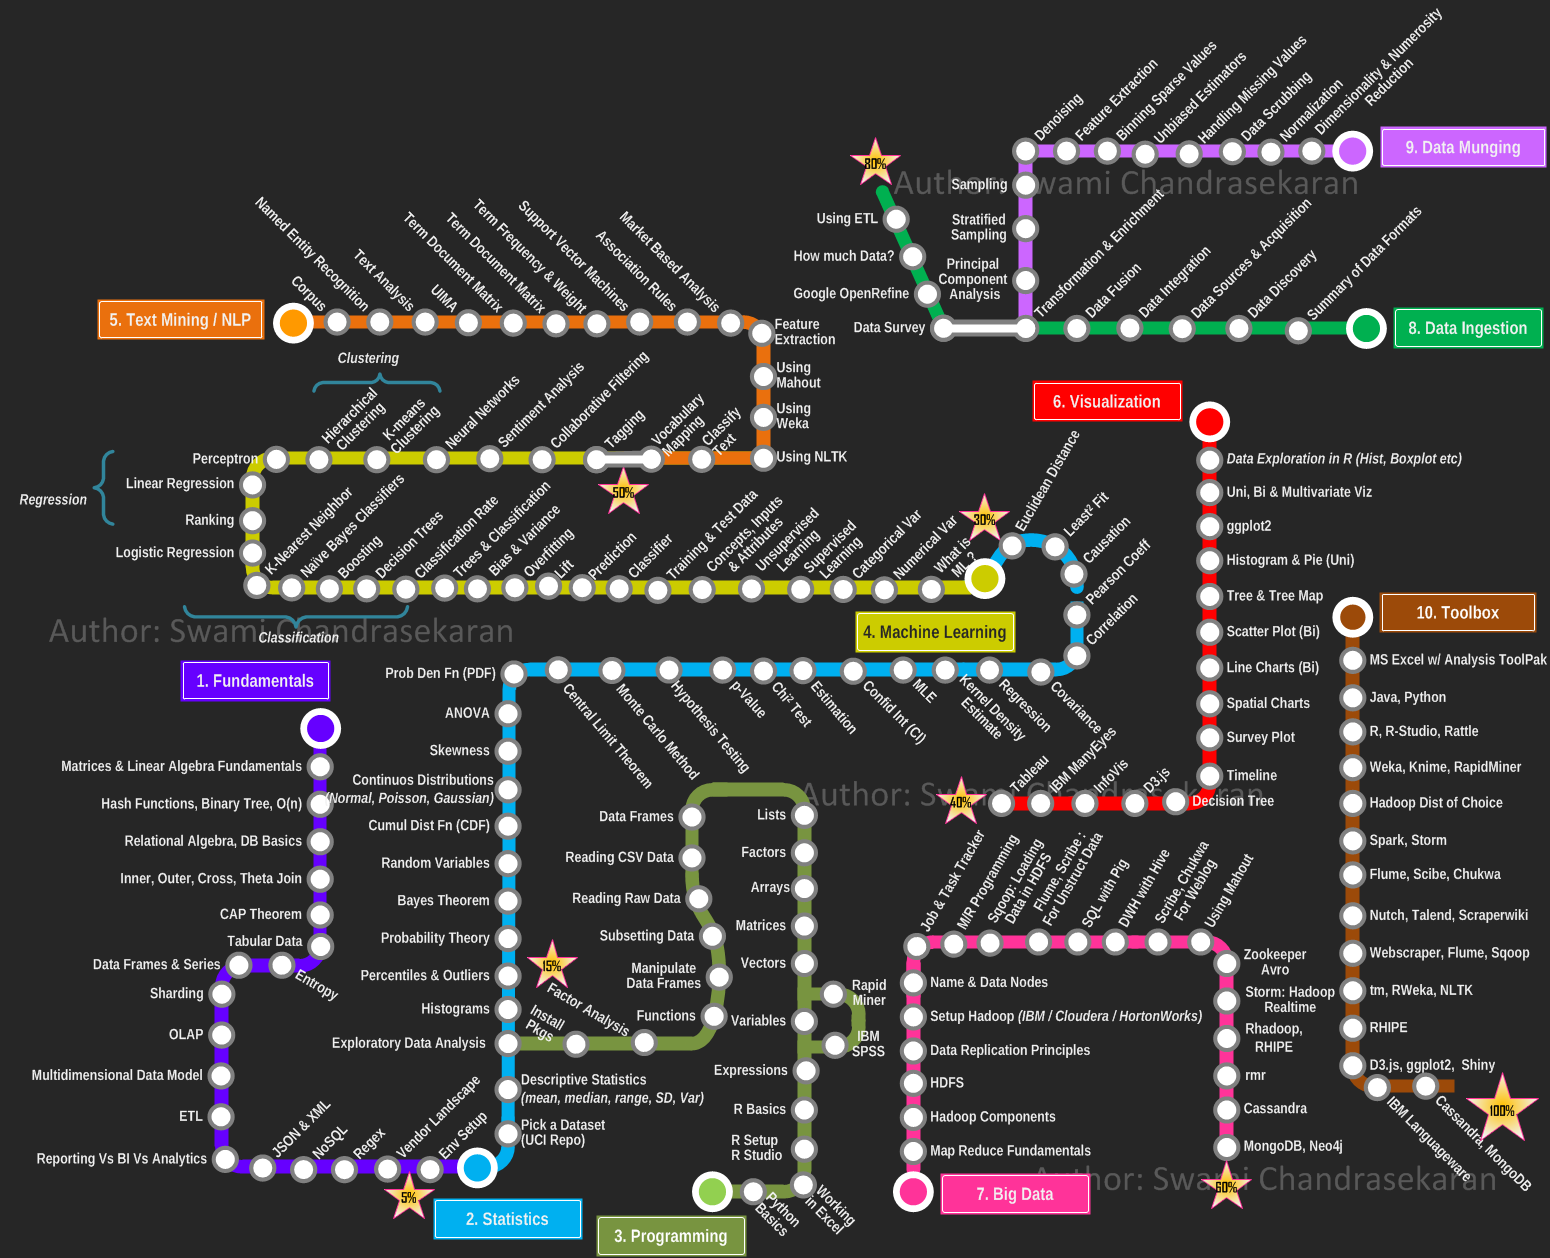
\includegraphics[width=\linewidth]{sections/images/RoadToDataScientist1.png}
    \caption{Road to Data Scientist}
    \label{RoadToDataScience}
\end{figure}


Comparison of \lstinline|R|, \lstinline|python|:focus on different aspects of `Statistics':
\begin{itemize}[topsep=2pt,itemsep=0pt]
    \item Differnece in programming philosophy: \lstinline|R| for data analysis and \lstinline|python| for data processing
    \item Difference in operating domain: \lstinline|R| for statistical programming while \lstinline|python| for general programming.
\end{itemize}



\subsection{Basic R. Manipulation}


\subsubsection{Installation and Maintenance of R.}
\begin{point}
    \textbf{Installing and Updating} 
\end{point}

\noindent  \lstinline|R.|: update by delete old version and install new version.
\begin{itemize}[topsep=2pt,itemsep=0pt]
    \item In CRAN (The Comprehensive \lstinline|R| Archive Network):\index{CRAN (The Comprehensive R Archive Network)} \url{https://cran.r-project.org}
    \item In Mirror@TUNA: \url{https://mirrors.tuna.tsinghua.edu.cn/CRAN}
\end{itemize}

\noindent RStudio: \url{https://www.rstudio.com}


\begin{point}
    \textbf{Running}  \lstinline|R.| \textbf{command} :
\end{point}

\begin{itemize}[topsep=2pt,itemsep=0pt]
    \item In \lstinline|R.| GUI\index{GUI (Graphical User Interface)};
    \item In \lstinline|R.| command line terminal;
    \item \lstinline|R. CMD BATCH|;
    \item \lstinline|Rscript|;
        \begin{itemize}[topsep=2pt,itemsep=0pt]
        \item Use \lstinline|>| to redirect output(overwrite);
        \item Use \lstinline|>>| to append output.
        \end{itemize}
\end{itemize}



\begin{point}
    \lstinline|R.| \textbf{package library}: packages are collection of \lstinline|R.| functions (as well as test data and sample code).
\end{point}

\begin{itemize}[topsep=2pt,itemsep=0pt]
    \item \lstinline|.libPaths()| show package library location\footnote{Unlike in \lstinline|C| or \lstinline|python| where \lstinline|.| is an operator, \lstinline|.| in \lstinline|R.| is just a common character, without special meaning.
    
    This feature can be used in naming self-defined functions: use \lstinline|.FUN_NAME1| for within-project function while \lstinline|FUN_NAME2| for external interface.} ;
    \item \lstinline|library('PACKAGE_NAME1','PACKAGE_NAME2',...)| load packages.
    \item \lstinline|install.packages('PACKAGE_NAME1','PACKAGE_NAME2',...)| install package from CRAN/mirrors;
    \item \lstinline|installed.packages()| show all installed packages;
    \item \lstinline|updata.packages(checkBuilt = TRUE, ask = FALSE)| update installed packages;
\end{itemize}

\begin{point}
    \textbf{Working directory}  manipulation:
\end{point}

\begin{itemize}[topsep=2pt,itemsep=0pt]
    \item \lstinline|getwd()| get current working directory;
    \item \lstinline|setwd('TARGET_PATH')| set working directory (as an existing path).
    \item \lstinline|dir()| show current directory.
\end{itemize}

\begin{point}
    Recommended \lstinline|R.| \textbf{Project Organization} : working directory organized like
\end{point}

\begin{itemize}[topsep=2pt,itemsep=0pt]
    \item \lstinline|data/| folder for structured original dataset;
    \item \lstinline|result/| folder for output result;
    \item \lstinline|presentation/| folder for result representing slides/reports/etc.;
    \item \lstinline|.r| project file $ \times n $.
\end{itemize}

\begin{point}
    Looking for \textbf{Help/Example}  of function:
\end{point}

\begin{itemize}[topsep=2pt,itemsep=0pt]
    \item \lstinline|?FUN_NAME()|;
    \item \lstinline|help('FUN_NAME')|;
\end{itemize}

\subsubsection{Data Structure and Basic Manipulation in R.}

\begin{point}
    Atomic Classes
\end{point}
\begin{itemize}[topsep=2pt,itemsep=0pt]
    \item \lstinline|'abc'| Character;
    \item \lstinline|3L| Integer;
    \item \lstinline|2.4| Numeric;
    \item \lstinline|TRUE,FALSE,T,F| Logical;
    \item Special types: \lstinline|NA|, \lstinline|NaN|, \lstinline|NULL|, \lstinline|Inf|
\end{itemize}

\begin{point}
    Operators
\end{point}
\begin{itemize}[topsep=2pt,itemsep=0pt]
    \item Numerical Operators: \lstinline|+|, \lstinline|-|, \lstinline|*|(multiply by column), \lstinline|/|, \lstinline|%*%|(matrix multiply), \lstinline|^|, \lstinline|%%|(remainder operate);
    \item Logical Operators: \lstinline|==|,etc.; \lstinline|&| and \lstinline{|} for common operator, \lstinline|&&| and \lstinline{||} for comparing the first element;
    \item Round a numeric:
    \begin{itemize}[topsep=2pt,itemsep=0pt]
        \item \lstinline|as.integer()|, round towards 0
        \item \lstinline|trunc()|
        \item \lstinline|ceiling()|
        \item \lstinline|floor()|
        \item \lstinline|round(NUMBER_TO_ROUND,digits = DIGITS)|
    \end{itemize}
\end{itemize}

\begin{point}
    Type Conversion
\end{point}

\begin{itemize}[topsep=2pt,itemsep=0pt]
    \item First need to meet the need of 
\end{itemize}

    
    Key Criterion: when converting mixed type in to the same type, use the type with more compatibility.
\begin{itemize}[topsep=2pt,itemsep=0pt]
    \item Logical $ \to $ Numeric: 
\end{itemize}

    

\begin{point}
    Data Structure
\end{point}
\begin{itemize}[topsep=2pt,itemsep=0pt]
    \item \textbf{Atomic Vector} : Column vector is the \textbf{basic} data structure in \lstinline|R.| (scalar is length=1 vector).
    
    Only data of the same class can be held in one vector.
    
    Initialization:
    \begin{itemize}[topsep=2pt,itemsep=0pt]
        \item Ordinary way: 
        \begin{itemize}[topsep=2pt,itemsep=0pt]
            \item \lstinline|c(1,2,3)|, \lstinline|c(T,FALSE,TRUE)|, \lstinline|c('a',NA,'b')|
            \item \lstinline|vector(mode = MODE,length = LENGTH)|
            \item \lstinline|logical(LENGTH)| return \lstinline|FALSE| vector 
        \end{itemize}
        
        where \lstinline|c()| for `combine'; 
        
        \lstinline|c()| combines all things into one vector, e.g. \lstinline|c(c(1,2,3),c(1,2))=(1,2,3,4,5)|.
        \item Sequence vector: 
        \begin{itemize}[topsep=2pt,itemsep=0pt]
            \item \lstinline|1:3.5=c(1,2,3)|, \lstinline|3:1=c(3,2,1)|
            \item \lstinline|seq(from, to ,by, length.out)|, \lstinline|length.out| for total vector length;
            \item \lstinline|rep(SEQ_TO_REP, times, lenght.out ,each)|, used in $ k $-fold cross validation labelling.
        \end{itemize}
    \end{itemize}
    
    Operations:
    \begin{itemize}[topsep=2pt,itemsep=0pt]
        \item between vectors of different length \lstinline|SHORT| and \lstinline|LONG|: First \lstinline|SHORT <- rep(SHORT,|\\\lstinline| length.out=length(LONG))|. Then operate \lstinline|SHORT| and \lstinline|LONG|.
        \item Element access: \lstinline|a[i]|
    \end{itemize}
    
         
    \fbox{
        \begin{minipage}{0.9\linewidth}

    \textbf{Vectorized Operation}: All operation in \lstinline|R.| are based on vector, and vectorized operation is Parallel Arithmetic, which is \textbf{much faster} than loop such as \lstinline|for| $ \longrightarrow $ Consider using vectorized opertion when writing code for \textbf{Speed}! Detail see \autoref{SubSubSectionVectorizedOperation}.
        \end{minipage}
    }

    \item \textbf{Factor} : A special kind of `vector' in \lstinline|R.|, used to label discrete categorical data.\footnote{Factor vector is stored as integer vector.}
    
    Initialization:

    \lstinline|factor(FACTOR_SEQ, levels = FACTOR_LEVEL, labels = ...)|, \lstinline|FACTOR_LEVEL| is the `rank' of each factor, \lstinline|labels| is the `tag' of levels. 

    A quick way to factorize a numeric vector \lstinline|x| by interval division:
    
    \lstinline|cut_number(x, NUM_OF_LEVELS)|

    \item \textbf{Matrix} : Only data of the same class can be held in one matrix.
    
    Initilaization:
    
    \lstinline|matrix(DATA_SEQ, nrow, ncol, byrow = FALSE, dimnames = NULL)|
    
    If \lstinline|length(DATA_SEQ) < nrow*ncol|, then \lstinline|DATA_SEQ| is repeated with \lstinline|length.out=nrow*ncol|. 
    
    Default: fill by column (because matrix is stored by column).

    Operation:
    \begin{itemize}[topsep=2pt,itemsep=0pt]
        \item Common operators \lstinline|+-*/^| etc. operate in column-by-column mode (vectorized operation).
        \item Binding matrix: \lstinline|cbind| for \lstinline|[A,B]| and \lstinline|rbind| for \lstinline|[A;B]|
        \item Transpose: \lstinline|t()|
        \item Matrix multiplication: \lstinline|%*%|
        \item Inverse matrix: \lstinline|solve()| (The essence of inversion is solving linear equations)
        \item Diagonal matrix:
        \begin{itemize}[topsep=2pt,itemsep=0pt]
            \item \lstinline|diag(VECTOR)| returns a matrix $ \mathrm{diag}\{ $\lstinline|VECTOR|$ \} $
            \item \lstinline|diag(MATRIX)| returns the diagonal element vector
        \end{itemize}
        \item Element access: \lstinline|a[i,j]|, \lstinline|a$OBJECT_NAME|
        \item Dimension: \lstinline|dim()|, \lstinline|nrow()|, \lstinline|ncol()|
        \item Rank: \lstinline|qr(MATRIX)$rank|
        % \item 
    \end{itemize}
    
    \item \textbf{List} : A pack containing various datatype, generally also a kind of vector(but not atomic vector)
    
    Initialization: \lstinline|list(OBJECT1,OBJECT2,...)|

    Element access: \lstinline|a[[i]]|
    \item \lstinline|data.frame|: `Mixture' of matrix and list. \lstinline|data.frame| is actually a kind of list(with some constraint), organized in the shape of matrix (but allowing different datatype for different columns, each column is a list object).
    
    Each column of \lstinline|data.frame| has name: \lstinline|names(DATA_FRAME)|, \lstinline|colnames(DATA_FRAME)|

    Element access: \lstinline|a[i,j]|, \lstinline|a[[i]]|, \lstinline|a$COL_NAME|
\end{itemize}

    
\begin{point}
    Data Read \& Write
\end{point}
\begin{itemize}[topsep=2pt,itemsep=0pt]
    \item Common R\&W: \lstinline|read.|/\lstinline|write.|
    \begin{itemize}[topsep=2pt,itemsep=0pt]
        \item \lstinline|read.table(FILE_NAME,header = FALSE,sep,colClasses,stringAsFactors = FALSE)|
        \item[${\color{red}\star }$] \lstinline|read.csv()| basically the same as \lstinline|read.table|
        \item[${\color{red}\star }$] \lstinline|write.table(DF,FILE_NAME,sep,row.names=FALSE)|
        \item \lstinline|readxl::read_xlsx(FILE_NAME,sheet = SHEET_NUM,range = 'RANGE')|
    \end{itemize}

    Some relative arguments:
    \begin{itemize}[topsep=2pt,itemsep=0pt]
        \item \lstinline|quote="'"|, use \lstinline|'| to quote/identify string, set \lstinline|quote=''| to avoid misread strings such as `Levene's Test'
        \item \lstinline|encoding='UTF-8'|, char encoding system, used especially for dataset containing CJK char.
        \item \lstinline|nrows=LINE_NUM| read first \lstinline|LINE_NUM| lines
        % \item 
    \end{itemize}

    \item Large Data Read \& Write: 
    \begin{itemize}[topsep=2pt,itemsep=0pt]
        \item preset \lstinline|colClasses|
        
\begin{lstlisting}[language=R]
temp.dat <- read.table(FILE_NAME, nrows = 100)
classes <- sapply(temp.dat, class)
dat <- read.table(FILE_NAME, colClasses = classes)
\end{lstlisting}
        \item \lstinline|readr::read_delim(FILE_NAME,delim=SEP)| can speed up
    \end{itemize}
    
    \item Text Write: \lstinline|sink(FILE_NAME,append=FALSE)|, write output into a file, the same as \lstinline|>| in terminal.
    \item \lstinline|.RData| Binary Format Read \& Write: RW in \lstinline|.RData| format, fast to load.
    \begin{itemize}[topsep=2pt,itemsep=0pt]
        \item \lstinline|save(DF,file = FILENAME)|
        \item \lstinline|load(FILE_NAME)|
    \end{itemize}
\end{itemize}

    




\subsubsection{Functions and Control Flow}
\begin{point}
    Program Speed:
\end{point}

\lstinline|system.time({COMMAND})|

\begin{point}
    Function Call
\end{point}
\begin{itemize}[topsep=2pt,itemsep=0pt]
    \item \lstinline|FUN_NAME(ARGUs)|
    \item \lstinline|do.call('FUN_NAME',LIST_OF_ARGUs)|, look for a function naming \lstinline|FUN_NAME| in \lstinline|R.| and call. 
    \item \lstinline|a % NEW_OPRTR % b| to call self-defined binary operator.
    \item \lstinline|'*'| etc. used in \lstinline|apply(FUN = '*')|
    \item \lstinline|R.| allows auto-completion to \lstinline|ARGUs|, e.g. \lstinline|rep(0,length.out=10)| = \lstinline|rep(0,length=0)|
\end{itemize}


\begin{point}
    Function Definition
\end{point}

\begin{rcode}
    Basic function definition in \lstinline|R.|
\begin{lstlisting}[language=R]
FUNC_NAME <- function(ARG1 = ARG1_DEF_VALUE , ARG2, ...) {
    FUNCTION_BODY
}
\end{lstlisting}
\end{rcode}

More key elements in \lstinline|funtion{}|
\begin{itemize}[topsep=2pt,itemsep=0pt]
    \item \lstinline|return(RETURN_OBJ)| at the end of function, without \lstinline|return()|, output the last line
    \item \lstinline|stopifnot(COND1,COND2,...)| at the beginning of function, used to test \lstinline|ARG| class
    \item \lstinline|stop(ERROR_MESG)| output error message
    \item \lstinline|...| as a special argument
    \begin{itemize}[topsep=2pt,itemsep=0pt]
        \item Pass \lstinline|...| to another func in this function
        \item Handle arbitrary number of input
    \end{itemize}
    \item Function can be defined within function
    \item Function is a kind of variable $ \longrightarrow $ used in \lstinline|apply|, \lstinline|sapply| etc. for vectorized programming.
    \item Anonymous function: used in \lstinline|sapply(X,FUN=function(){STATs})| for quick definition
    \item \lstinline|FUNC_NAME| can be used for new-defined binary operator as \lstinline|'%NEW_OPRTR%' <- function()|
\end{itemize}


\begin{point}
    Flow Control
\end{point}

\begin{itemize}[topsep=2pt,itemsep=0pt]
    \item \lstinline|if| and \lstinline|else if|, example:
\begin{lstlisting}[language=R]
if(COND1) {
    STATEMENT
} else if(COND2) {
    STATEMENT
} else {
    STATEMENT
}
\end{lstlisting}
    \item \lstinline|ifelse(COND,IF_YES_STAT,IF_NO_STAT)| a vectorized version of \lstinline|for+if else|.

    \item \lstinline|for|: Loop in \lstinline|R.| is \textbf{Extremely Slow}, avoid loop, use \textbf{vectorized operation}.  
\begin{lstlisting}[language=R]
for(VAR in SEQ) {
    STATEMENT
}
\end{lstlisting}
    \item \lstinline|switch(TEST_EXPR,CASE1 = RETN1,CASE2 = RETN2,...)|
 
    
        
    

\end{itemize}







\subsubsection{Vectorized Operation}\label{SubSubSectionVectorizedOperation}
\begin{itemize}[topsep=2pt,itemsep=0pt]
    \item \lstinline|apply()| function series:
\begin{itemize}[topsep=2pt,itemsep=0pt]
    \item \lstinline|apply(MAT,MARGIN,FUN)| for matrix apply, \lstinline|MARGIN=1| for each row, \lstinline|2| for each column
    \item \lstinline|lapply(LIST,FUN)| for list/\lstinline|data.frame|, apply \lstinline|FUN| on each list elements,\lstinline|list| returned
    \item[$ \color{red}\star $] \lstinline|sapply(X,FUN)| for list/\lstinline|data.frame| apply+simplify, \lstinline|vector/matrix/list| returned
    \item \lstinline|tapply(X,INDEX,FUN)|: for each index, use \lstinline|FUN| respectively.
    \item \lstinline|mapply(FUN,ARGU_OF_FUN)|, use argument name to label \lstinline|ARGU_OF_FUN|, or causes bad readability. 
    
    Example:
\begin{lstlisting}[language=R]
mapply(function(x,y,z,k){(x+k)^(y+z)} , x = ,y = ,z = ,k = )
\end{lstlisting}
    \end{itemize}

    \item \lstinline|Vfunc <- Vectorize(FUNC_NAME)|: define vectorize version of function.
    \item \lstinline|with()| and \lstinline|within()|:
    \begin{itemize}[topsep=2pt,itemsep=0pt]
         \item \lstinline|with(DF,aggregate(PART,by,FUN))|
        \item \lstinline|with(DF,STATE),within(DF,STATE)|,
     \lstinline|within| allows new column append
    \end{itemize}
    \item \lstinline|outer(VEC1,VEC2,FUN)|: A Two-variate extension of \lstinline|mapply()|, output wedge of two vectors.
    \item \lstinline|ifelse(COND,YES_STAT,NO_STAT)|, vectorization supported.
\end{itemize}





\subsubsection{Subsetting}
\begin{itemize}[topsep=2pt,itemsep=0pt]
    \item By position: \lstinline|x[RANGE]|
    \begin{itemize}[topsep=2pt,itemsep=0pt]
        \item \lstinline|x[4]|
        \item \lstinline|x[-4]|: without the $ 4^\mathrm{th} $ item (different from \lstinline|python|, where selects reciprocal $ \mathrm{4^{th}}  $ element).
        \item \lstinline|x[2:4]|
        \item \lstinline|x[c(1,2,5)]|
    \end{itemize}
    \item By name: \lstinline|x[,'COL_NAMEs']|, \lstinline|x[,'COL_NAME1':'COL_NAME2']|
    \item By condition: basically, \lstinline|x[LOGI_VEC]|
    \begin{itemize}[topsep=2pt,itemsep=0pt]
        \item \lstinline|x[x==10]|
        \item \lstinline|x[x %in% c(1,3,4)]|, linear search, not based on hash algorithm\footnote{If really needed, use \lstinline|env()| to reset environment.}.
    \end{itemize}

    Usually used for conditional selection of \lstinline|data.frame|
    \item Subsetting for \lstinline|data.frame| and list: \lstinline|x[[RANGE]]|


    Simplified/Preserved subsetting: whether preserved datatype, e.g. df $ \to $ df (preserved) v.s. df $ \to $ vector (simplified).
\begin{table}[H]
    \centering
    \renewcommand\arraystretch{1.15}
    \begin{tabular}{lll}
        \hline
        DataType&Simplified&Preserved\\
        \hline
        vector&\multicolumn{2}{c}{\lstinline|x[[1]]]| / \lstinline|x[1]|}\\
        list&\lstinline|x[[1]]|&\lstinline|x[1]|\\
        factor&\lstinline|x[1:4,drop=T]|&\lstinline|x[1:4]|\\
        matrix&\lstinline|x[,1]|&\lstinline|x[,1,drop=F]|\\
        \lstinline|data.frame|&\lstinline|x[,1]|,\lstinline|x[[1]]|&\lstinline|x[,1,drop=F]|,\lstinline|x[1]|\\
        \hline
    \end{tabular}
    \caption{Simplified/Preserved subsetting}
\end{table}
    \item Other subsetting:
    \begin{itemize}[topsep=2pt,itemsep=0pt]
        \item \lstinline|%in%| 
        \item \lstinline|unique()|, return with each element appears only one times
        \item \lstinline|duplicated()|, \lstinline|TRUE| when appear the $ n>1 $ times
        \item \lstinline|which(x==4)|, return position of matched element
        \item \lstinline|which.min()|, \lstinline|which.max|, \lstinline|min()|, \lstinline|max()|
        \item \lstinline|grep(REGEX,X,value)|, search for elements with \lstinline|REGEX| pattern: \lstinline|value=F| returns position, \lstinline|value=T| returns elements, \lstinline|grepl(REGEX,X)| returns logical vector
        \item \lstinline|match(TO_BE_MATCHED,TARGET)|, returns the index of elements of \lstinline|TO_BE_MATCHED| in \lstinline|TARGET|
        
        \begin{rcode}
            Example:
\begin{lstlisting}[language=R]
vec1 <- c('a','a','b','b','d','d','b')
vec2 <- c('d','a','b')
match(vec1,vec2)
> [1] 2 2 3 3 1 1 3
\end{lstlisting}
        \end{rcode}
        \item \lstinline|subset(X,...)|, \lstinline|...| a series of select criterion. \textbf{not} allowed: \lstinline|subset(X,...) <- | 
    \end{itemize}
    \item Use subsetting to sample: \lstinline|DATA[sample(1:nrow(DATA),NUM_OF_SAMPLE,replace),]|, \lstinline|replace=T| for with replacement
\end{itemize}

\subsubsection{Data Manipulation With dplyr. And tidyr.}
    \lstinline|dplyr| and \lstinline|tidyr| are two useful package for data cleaning \& manipulation. Use package \lstinline|tidyverse| include both of them.

    \lstinline|tidyverse| for \lstinline|tidy|uni\lstinline|verse|, includes \lstinline|dplyr|, \lstinline|tidyr|, \lstinline|readr|, \lstinline|ggplot2|, \lstinline|stringr|, etc.

\begin{point}
    \lstinline|%>%| pipe in \lstinline|tidyverse|: functions in \lstinline|tidyverse| use \lstinline|FUNC(DF,...)|, where \lstinline|DF| can be passed on by \lstinline|%>%|.

\end{point}


\begin{point}
    \lstinline|dplyr| Package. 
\end{point}

\begin{itemize}[topsep=2pt,itemsep=0pt]
    \item Cheet Sheet: \url{https://nyu-cdsc.github.io/learningr/assets/data-transformation.pdf}
    \item \lstinline|select(DF,...)|, where \lstinline|...| can use column index/name range as in subsetting, or some helper function for advanced subsetting:
    \begin{itemize}[topsep=2pt,itemsep=0pt]
        \item matching position:
        \begin{itemize}[topsep=2pt,itemsep=0pt]
            \item \lstinline|everything()|
            \item \lstinline|last_col()|
        \end{itemize}
        \item matching column name:
        \begin{itemize}[topsep=2pt,itemsep=0pt]
            \item \lstinline|start_with('PATTERN')|, \lstinline|end_with('PATTERN')|, \lstinline|contains('PATTERN')|
            \item \lstinline|match('REGEX')|, column name with \lstinline|REGEX| pattern
            \item \lstinline|num_range('x',1:4)| delect column name \lstinline|c('x1','x2','x3','x4')|
            \item \lstinline|any_of(CHR_VEC)| select column from \lstinline|CHR_VEC|
        \end{itemize}
        \item \lstinline|where(FUN)|, select those \lstinline|FUN(COL_NAME)| returns \lstinline|TRUE|
    \end{itemize}
    \item \lstinline|filter(DATA,CONDs)|, select elements with \lstinline|CONDs| conditions
    \item \lstinline|arrange(DATA,COL)|, sort by \lstinline|COL|, \lstinline|arrange(DATA,desc(COL))| for descending order
    \item \lstinline|mutate(DATA,...)|, append new columns according to \lstinline|...| definition; \lstinline|transmute()| drops original columns.
    
    \lstinline|...| definition can use advanced window function:
    \begin{itemize}[topsep=2pt,itemsep=0pt]
        \item \lstinline|lead(COL)|,\lstinline|lag(COL)|, e.g. \lstinline|lead(COL)[i]|=\lstinline|COL[i+1]|, can use \lstinline|...=COL-lead(COL)| for differnetial
        \item \lstinline|dense_rank(COL)|, \lstinline|percent_rank(COL)| rank number
        \item \lstinline|ntile(COL,N)| break into \lstinline|N| groups labeling \lstinline|1:N|
        \item \lstinline|cume_dist(COL)|, \lstinline|cummean(COL)|, \lstinline|cumsum(COL)|, \lstinline|cummax(COL)|, \lstinline|cummin(COL)|, etc. cumulative value
    \end{itemize}
    
    \item \lstinline|summarise(data,...)|, \lstinline|...| for summarise function.

    \item Row selection:
    \begin{itemize}[topsep=2pt,itemsep=0pt]
        \item \lstinline|slice(DF,ROW_RANGE)|
        \item \lstinline|distinct(DF)| remove duplicated rows
        \item \lstinline|sample_frac(DF,FRAC,replace)|, sample \lstinline|FRAC| fraction from \lstinline|DF|
        \item \lstinline|sample_n(DF,N,replace)|, sample \lstinline|N| cases from \lstinline|DF|
        \item \lstinline|top_n(DF,AMOUNT,RANK_COL)| select \lstinline|AMOUNT| top ranking by \lstinline|RANK_COL| cases
    \end{itemize}
    \item Data combining see slides.
\end{itemize}

\begin{point}
    \lstinline|tidyr| Package
\end{point}
\begin{itemize}[topsep=2pt,itemsep=0pt]
    \item Cheet Sheet: \url{https://leadousset.github.io/intro-to-R/cheatsheet_tidy.pdf}
    \item \lstinline|gather(DF,key='KEY_NAME',value='VALUE_NAME',...,na.rm)|, melt a \lstinline|data.frame|. 
    
    e.g. \lstinline|gather(df,'KEY','VALUE',c('COL1','COL2','COL3'))| transfers \lstinline|...| as:
    \[
        \begin{matrix}
            \text{ID}&\text{COL1}&\text{COL2}&\text{COL3}\\
            1&a_1&b_1&c_1\\
            2&a_2&b_2&c_2\\
            \vdots&\vdots&\vdots&\vdots
        \end{matrix}
        \quad\to\quad
        \begin{matrix}
            \text{ID}&\text{KEY}&\text{VALUE}\\
            1&\text{COL1}&a_1\\
            2&\text{COL1}&a_2\\
            \vdots&\vdots&\vdots\\
            1&\text{COL2}&b_1\\
            2&\text{COL2}&b_2\\
            \vdots&\vdots\\
            1&\text{COL3}&c_1\\
            2&\text{COL3}&c_2\\
            \vdots&\vdots
        \end{matrix}
    \]
    \item \lstinline|spread(DF,key='KEY_NAME',value='VALUE_NAME')|, inverse of \lstinline|gather()|
    \item \lstinline|separate(DF,COL,into=SET_VEC,sep='REGEX')|, separate \lstinline|COL| into columns with name in \lstinline|SET_VEC|, sep according to \lstinline|sep|
    \item \lstinline|unite(DF,COL,SET_VEC,sep='')| inverse of \lstinline|separate()|
\end{itemize}

    


\subsection{Text Processing \& Text Mining}
    \begin{itemize}[topsep=2pt,itemsep=0pt]
        \item Data cleaning
        \item Data manipulation
        \item Information extraction: mode identifying/relation extraction
        \item Text mining: anaylzing token distribution, ignore word order
        \item NLP: concept identifying based on sentence; untimate goal: `understand' sentence meaning.
    \end{itemize}
    
    Tools for Text processing:
\begin{itemize}[topsep=2pt,itemsep=0pt]
    \item \lstinline|R.|: suitable for easy task 
    \item \lstinline|python.|: best
    \item \lstinline|java|: strong, but not suitable for deep learning
    \item \lstinline|c++|: fast, inadequate package
    \item \lstinline|Notepad++|/\lstinline|Vim|
\end{itemize}

    
        



\subsubsection{Basic Text Manipulation With stringr.}
\begin{point}
    \lstinline|R. base| \& \lstinline|stringr| package:
\end{point}

    The prior one is used more often

\begin{itemize}[topsep=2pt,itemsep=0pt]
    \item Cheet Sheet: \url{http://edrub.in/CheatSheets/cheatSheetStringr.pdf}
    \item \lstinline|str_length(STRING)|, \lstinline|nchar(STRING)|
    \item \lstinline|paste(...,collapse=NULL)|,\lstinline|str_c(...)|, both are vectorized operation
    
    Argument:
    \begin{itemize}[topsep=2pt,itemsep=0pt]
        \item \lstinline|sep|: sep between each \lstinline|...| corresponding elements, with \lstinline|collapse=NULL|, return a char vector
        \item \lstinline|collapse|: sep when combining \lstinline|collapse=NULL| vector elements, \lstinline|NULL| for not combining
        \item Special character: \lstinline|\t| tab, \lstinline|\r| \& \lstinline|\n| \& \lstinline|\r\n| new line, \lstinline|\xad| `-' at end on line for word-connecting
    \end{itemize}
    
    \item \lstinline|str_split(STRING,pattern='REGEX')|/\lstinline|strsplit()|, split string at \lstinline|REGEX| pattern fitted, list returned
    \item \lstinline|str_sub(STRING,start,end)|, \lstinline|substr()|. The \lstinline|start| char to \lstinline|end| char of string, use negative index as in \lstinline|python|.
     
    Can be used to replace: \lstinline|str_sub(...) <- REP_STR|
    \item \lstinline|str_locate_all('STRING',pattern='REGEX')|/\lstinline|str_match_all('STRING',pattern='REGEX')|

    \lstinline|grep(pattern='REGEX',x='STRING',value=T)|, search for elements with \lstinline|REGEX| pattern: \lstinline|str_locate_all()| or \lstinline|value=F|  returns position, \lstinline|str_match_all()| or \lstinline|value=T| returns elements.
    
    \item \lstinline|str_replace_all('STRING',pattern='REGEX',replacement='REP')|
    \lstinline|grepl(REGEX,X)| returns logical vector, include or not.
    \lstinline|str_extract_all('STRING',pattern='REGEX')|
    \item \lstinline|gsub(pattern='REGEX',replacement='REP',x='STRING')|, replace \lstinline|REGEX| field with \lstinline|REP|
    % \item Extracting word: 
    \item \lstinline|str_trim(...,side = )|, trim extra white space at \lstinline|side='both'|/\lstinline|'left'|/\lstinline|'right'|
    % \item Padding: \lstinline|str_pad()| append space
\end{itemize}




\subsubsection{Regular Expression}
    Regular expression is a text pattern/mode. abbr. regex/regexp. Regex is supported in most common language, same syntax used.

    Tutorial: \url{https://www.runoob.com/regexp/regexp-tutorial.html}

\begin{point}
    Key Elements
\end{point}

\begin{itemize}[topsep=2pt,itemsep=0pt]
    \item Literal: common char, e.g. \lstinline|a|. Include most char on keyboard. Upper/Lower case sensitive.
    \item Metacharacters: \lstinline!\^$.|?*+()[]{}!, use e.g. \lstinline|\.| to escape meaning.
    
    Note: when typing regex in programming language, sometimes use \lstinline|\\.|: \lstinline|\\.| $ \xrightarrow[]{\text{language interpreter}}  $ \lstinline|\.| $ \xrightarrow[]{\text{regex interpreter}}  $ identifying \lstinline|.|

    \item Character Class: \lstinline|[]|, identify one of elements in \lstinline|[]|. \lstinline|^| within \lstinline|[]| for $ \complement $. 
    \begin{itemize}[topsep=2pt,itemsep=0pt]
        \item e.g. \lstinline|gr[ae]y| identifies \lstinline|grey| and \lstinline|gray|.
        \item e.g. \lstinline|[0-9]| numbers, \lstinline|[a-zA-z]| letter
        \item e.g. \lstinline|q[^x]| matches \lstinline|question|, not matchs \lstinline|qxestion|, not matches \lstinline|Iraq|
    \end{itemize}

    character class shorthand
\begin{table}[H]
    \centering
    \renewcommand\arraystretch{1.15}
    \begin{tabular}{lll}
        \hline
        ShortHand&Meaning&Equivalant \lstinline|REGEX|\\
        \hline
        \lstinline|\d|&numeric digit&\lstinline|[0-9]|\\
        \lstinline|\D|&Not numeric digit&\lstinline|[^\d]|\\
        \lstinline|\w|&a word character&\lstinline|[a-zA_Z0-9_]|\\
        \lstinline|\s|&white space&\lstinline|[\t\r\n\f]|\\
        \hline
    \end{tabular}
\end{table}

    \item Wildcard(通配符): \lstinline|.| matches any single character except line break \lstinline|\r|,\lstinline|\n|
    \item Anchor(词边界/定位符): match `word boundary' (not the space at the start/end of string).
    
    \lstinline|^| string start, \lstinline|$| string end, \lstinline|\b| word boundary, \lstinline|\B| not-a-word-boundary position
    \item Repetition/Quantifier: here \lstinline|X| for some regex pattern like \lstinline|CHAR|, \lstinline|[]| etc.
    
\begin{table}[H]
    \centering
    \renewcommand\arraystretch{1.15}
    \begin{tabularx}{0.9\linewidth}{XXXX}
        \hline
        Greedy&$ \color{red}\star $ Reluctant&Possessive&Freq of Occurrence\\
        \hline
        \lstinline|X?|&\lstinline|X??|&\lstinline|X?+|& $ 0,1 $\\
        \lstinline|X+|&\lstinline|X+?|&\lstinline|X++|& $ \geq 1 $\\
        \lstinline|X*|&\lstinline|X*?|&\lstinline|X*+|& 0,$ >1 $\\
        \lstinline|X{n}|&\lstinline|X{n}?|&\lstinline|X{n}+|& $ n $\\
        
        \lstinline|X{n,}|&\lstinline|X{n,}?|&\lstinline|X{n,}+|& $ \geq n $\\
        \lstinline|X{n,m}|&\lstinline|X{n,m}?|&\lstinline|X{n,m}+|& $ [n,m] \qquad\qquad  $\\
        \hline
    \end{tabularx}
\end{table}

    Example: Search `foo' in `xfooxxxxxxfoo':
    \begin{itemize}[topsep=2pt,itemsep=0pt]
        \item Greedy: `xfooxxxxxxfoo' found at index 0-13
        \item[$ \color{red}\star $] Reluctant: `xfoo' found at index 1-4, `xxxxxxfoo' found at index 4-13
        \item Possessive: no match found (not usually used)
    \end{itemize}
    
    Example: regex match 'aaaa'
    \begin{itemize}[topsep=2pt,itemsep=0pt]
        \item 
    \end{itemize}
    
        
    \item Alternation \& Grouping \& Back Reference: \lstinline!XA|XB! identify \lstinline|XA| or \lstinline|XB|, use grouping \lstinline|()| to set boundary of XA,XB.
    
    Use \lstinline|\n| for back reference the $ n^\mathrm{th}  $ group. 
\begin{rcode}
    Example: search for immediate repeat word in a sentence
\begin{lstlisting}[language=R]
(\b[a-zA-Z]+\b) \1
\end{lstlisting}
\end{rcode}
    \item Lookaround: 
    \begin{itemize}[topsep=2pt,itemsep=0pt]
        \item LookAhead: \lstinline|(?<=X)q|
        \item LookBehind: \lstinline|q(?=X)|
    \end{itemize}
    
        
\end{itemize}

    
\subsubsection{Web Scraping}
    Basic elements of web page:
\begin{itemize}[topsep=2pt,itemsep=0pt]
    \item HTML (HyperText Markup Language): structure and content of page
    \item CSS (Cascading Style Sheet): page style.
    \item JavaScript: functionality, interaction
\end{itemize}

        
Basic \lstinline|html| document format:
\begin{rcode}
\begin{lstlisting}[language=R]
<!DOCTYPE html> # an html document
<html> # html page begin
<head> # head elements declare
<meta charset="utf-8">
<title> TITLE OF WEB PAGE </title>
</head>
<body> # html body begin
 
<h1> HEADING 1 </h1>
<p class='TEST_TEXT'> PARAGRAPH 1 </p>
 
</body>
</html>
\end{lstlisting}
\end{rcode}

    We can use elements like \lstinline|<p>| or \lstinline|class| to extract page information.

\begin{point}
    Web Scraping with \lstinline|rvest.|
\end{point}

\begin{itemize}[topsep=2pt,itemsep=0pt]
    \item \lstinline|pge <- read_html('URL')|: page read
    
    Proxy set: \lstinline|Sys.setenv(https_proxy='http://127.0.0.1:7890')|
    \item \lstinline|pge %>% html_elements(css='.CSS_CLASS_NAME') %>% html_text()|: basic scraping. use SelectGadget tool for help finding proper css label.
\end{itemize}

% \subsubsection{Word Segmentation}



\subsection{Graphic in R.}

\subsubsection{R::base Plotting}

    Plot function in \lstinline|R::base|:\index{Plot Parameters in R.}
\begin{lstlisting}[language=R]
plot(X,Y) # scatter/line plot of Y-X
plot(FUNC_OBJ, from = , to = ) # function plot ranging in c(from, to)
plot(FACTOR) # barplot of factors
plot(FACTOR, Y) # boxplot of numeric v.s. levels of factor
plot(DATA.FRAME) # correlation plot
plot(ANY_PLOTTABLE_OBJ) # plot any plottable object 
\end{lstlisting}

\begin{itemize}[topsep=2pt,itemsep=0pt]
    \item Plot saving: first open a plotting device, then make plot and close the device
\begin{lstlisting}[language=R]
pdf("PLOT_FILE_NAME.pdf", FIG_HEIGHT, FIG_WIDTH)
plot(PLOT_PARAM)
dev.off()
\end{lstlisting}
    \item \lstinline|plot()| plotting parameters:
    \begin{itemize}[topsep=2pt,itemsep=0pt]
        \item \lstinline|main = | string for title; or use \lstinline|title('TITLE')| as the next command
        \item \lstinline|sub = | string for subtitle;
        \item \lstinline|xlab = , ylab = | string axis labels;
            \item adding \LaTeX expression as text: use \lstinline|main = expression(PLOTMATH_EXPRESSION)|, use \lstinline|?plotmath| to look for possible symbols
        \item \lstinline|xlim = , ylim = | axis range, e.g. use \lstinline|xlim = c(0,100)|
        \item \lstinline|type = | value taken in \lstinline|c('p', 'l', 'b', 'o', 's', 'h')| for plot \textbf{type}
        \begin{figure}[H]
            \centering
            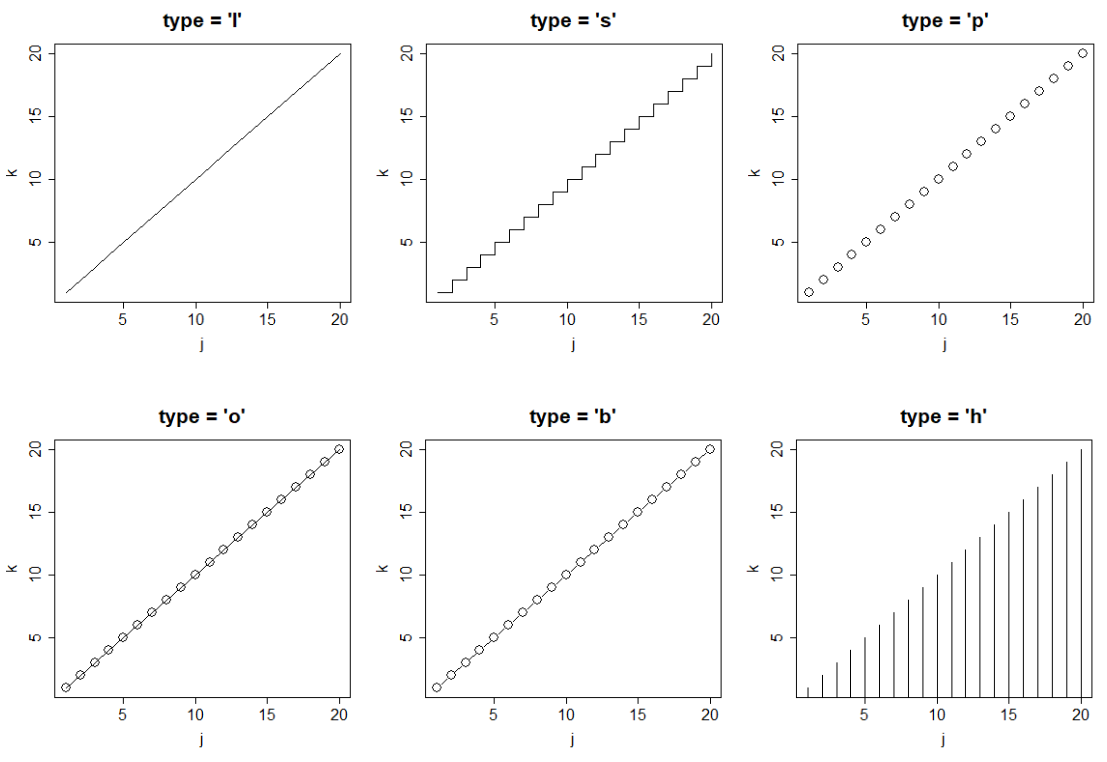
\includegraphics[width=0.8\linewidth]{sections/images/2022-08-18-11-24-35.png}

            \label{}
        \end{figure}
        
        \item \lstinline|pch = | \textbf{p}oint \textbf{ch}aracter, value taken in \lstinline|0:25| for defulat point charaters listed below, or use (vector of) charater to specify, e.g. \lstinline|pch = c('❄')|
        \begin{figure}[H]
            \centering
            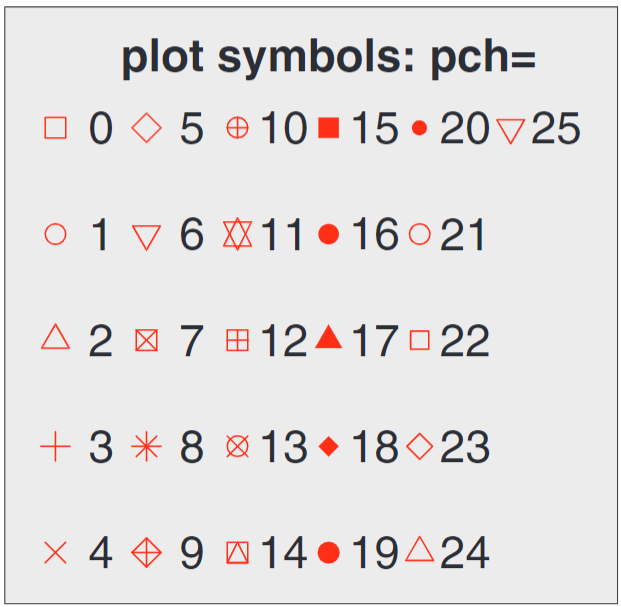
\includegraphics[width=0.3\linewidth]{sections/images/2022-08-18-11-14-15.png}

            \label{}
        \end{figure}

        \item \lstinline|lty = | \textbf{l}ine \textbf{ty}pe, value taken in \lstinline|1:6| (0 for not shown)
        \begin{figure}[H]
            \centering
            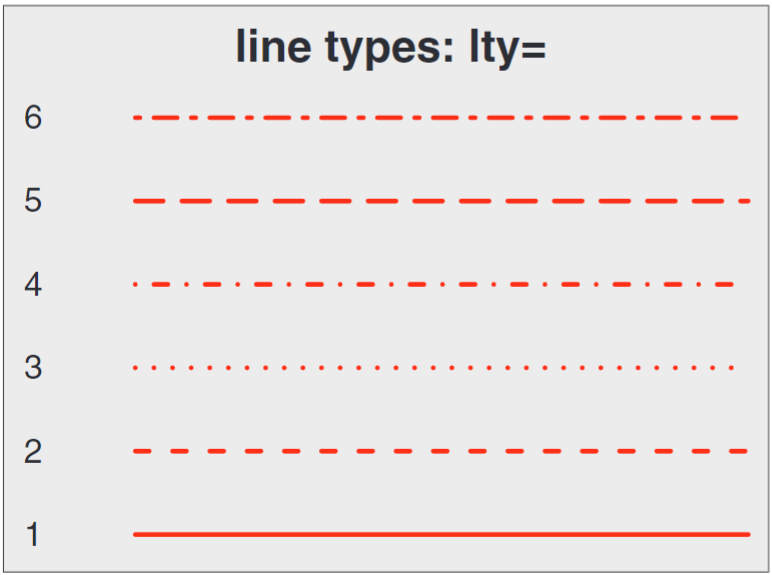
\includegraphics[width=0.4\linewidth]{sections/images/2022-08-18-11-15-34.png}

            \label{}
        \end{figure}

        \item \lstinline|cex = | \textbf{c}haracter \textbf{ex}pansion, relative size with 1 as baseline and default. 
        
        Some derivative function to control size of other plotting elements:
        \begin{itemize}[topsep=2pt,itemsep=0pt]
            \item \lstinline|cex.axis = | relative size of axis node text
            \item \lstinline|cex.lab = | relative size of labels
            \item \lstinline|cex.main = | relative size of title 
            \item \lstinline|cex.sub = | relative size of subtitle 
        \end{itemize}
        
        \item \lstinline|lwd = | \textbf{l}ine \textbf{w}i\textbf{d}th, relative width of line with 1 as baseline and default
        \item \lstinline|col = | \textbf{color} of elements in plot, value examples for color white:
        \begin{itemize}[topsep=2pt,itemsep=0pt]
            \item Index: \lstinline|col = 1| predefined color in \lstinline|R.| 
            \item Color name: \lstinline|col = 'white'|, use \lstinline|colors()| to see all available color names
            \item Hexadecimal code: \lstinline|col = '#FFFFFF'|
            \item RGB code: \lstinline|col = rgb(1,1,1)|, \lstinline|col = rgb(255,255,255, maxColorValue = 255)|
            \item HSV code: \lstinline|col = hsv(0,0,1)|
        \end{itemize}

        \lstinline|col = | can accept vector for various colors, or acccept some function for continuous colors:
        \begin{itemize}[topsep=2pt,itemsep=0pt]
            \item Discrete color: \lstinline|col = c('red','blue')|, or use \lstinline|col = df$GROUP| to color different groups
            \item Continuous color function: \lstinline|rainbow(NUM_OF_COLORS)|, \lstinline|heat_colors()|, \lstinline|terrain.colors()|, \lstinline|topo.colors()|, \lstinline|cm.colors()|
        \end{itemize}

        Some derivative function to control color of other plotting elements:
        \begin{itemize}[topsep=2pt,itemsep=0pt]
            \item \lstinline|col.axis = | color of axis node text
            \item \lstinline|col.lab = | color of labels
            \item \lstinline|col.main = | color of title 
            \item \lstinline|col.sub = | color of subtitle 
            \item \lstinline|bg = | color of background
        \end{itemize}

        \item \lstinline|font = | \textbf{font} used in plot, with 1 = plain, 2 = bold, 3 = italic,
        4 = bold italic

        Some derivative function to control font of other plotting elements:
        \begin{itemize}[topsep=2pt,itemsep=0pt]
            \item \lstinline|font.axis = | font of axis node text
            \item \lstinline|font.lab = | font of labels
            \item \lstinline|font.main = | font of title 
            \item \lstinline|font.sub = | font of subtitle 
            \item \lstinline|ps = | baseline font \textbf{p}oint \textbf{s}ize, i.e. text size = \lstinline|ps*cex|
            \item \lstinline|family = | extra text type, value taken in \lstinline|c('serif', 'sans', 'mono')|m etc. use \lstinline|names(pdfFonts())| to see possible font families
        \end{itemize}
        \item \lstinline|bty = | \textbf{b}ox \textbf{ty}pe of the box surrounding the figure. Value taken in \lstinline|c('o', '7', 'L', 'U', 'C', 'n')| 
    \end{itemize}
    \item \lstinline|axis()| parameters for axis settings: after using \lstinline|xaxt = 'n'| or \lstinline|yaxt = 'n'| to remove correponding axis when executing \lstinline|plot()|, other variation of axis could be made by using \lstinline|axis()|
    \begin{itemize}[topsep=2pt,itemsep=0pt]
        \item \lstinline|axis(1)| for creating $ x $ aixs, \lstinline|axis(2)| for creating $ y $ aixs. Here we would use $ x $ axis in the following parts.
        \item \lstinline|aixs(1, at = )| to specify ticks.
        \item \lstinline|plot(las = )| to specify rotation of ticks, value taken in \lstinline|c('Parallel', 'Horizontal', 'Perpendicular', 'Vertical')|
        \item \lstinline|plot(xlim = c( , ), ylim = c( , ))| for axis limits
        \item \lstinline|plot(log = )| for log transfrom on axis, value taken in \lstinline|c('x', 'y', 'xy')|. 
    \end{itemize}
    
        

    \item \lstinline|legend()| parameters:
    \begin{itemize}[topsep=2pt,itemsep=0pt]
        \item \lstinline|x = | position of legend, value taken in \lstinline|c("top", "bottom", "topleft", "topright", "bottomleft", "bottomright")|
        \item \lstinline|inset = |
        \item other parameters are set following the setting in \lstinline|plot|. An example:
\begin{lstlisting}[language=R]
legend("bottomright", legend = c("red", "green"), lty = c(2,4), lwd = 3, col = c("red", "green"))
\end{lstlisting}

    \end{itemize}

    \item \lstinline|text(X_COOR, Y_COOR, labels = TEXT)| parameters for adding text in figure. An application is \lstinline|text(df$X, df$Y, labels = df$Z)| to label each point.
    \begin{itemize}[topsep=2pt,itemsep=0pt]
        \item \lstinline|pos = | \textbf{pos}ition of text around the coordinate point, value taken in \lstinline|c(1,2,3,4)| 
    \end{itemize}
    
    \item \lstinline|lines()| to put an extra line on existing figure (device). Parameters are similarly set as \lstinline|plot()|
    
    \item \lstinline|par()| to set global \textbf{par}ameters. An example to put 3 different figure in the same device:
\begin{lstlisting}[language=R]
opar <- par(no.readonly = TRUE) # copy original setting
par(mfrow = c(1,3))
plot()
plot()
plot()
par(opar)
\end{lstlisting}

\end{itemize}

\begin{point}
    More Charts
\end{point}

\begin{itemize}[topsep=2pt,itemsep=0pt]
    \item \lstinline|barplot(counts, horiz, besides, ...)| for bar plot. Data should be first prepared by \lstinline|counts <- table(Y_TO_COUNT)|. 
    \item \lstinline|hist(x, breaks, freq, ...)| for histogram.
    \item \lstinline|plot(density(df, kernel = ), ...)| for density plot.
    \item \lstinline|boxplot(x, ...)| for box plot. use \lstinline|boxplot(x ~ GROUP, data = , ...)| to plot grouped boxplot
    \item \lstinline|dotchart(x, labels, groups, ...)| to compare \lstinline|x| value for categories
\end{itemize}


\subsubsection{R::ggplot2 Plotting}
    \lstinline|ggplot2|: \textbf{G}rammar of \textbf{G}raphics \textbf{plot} (2nd edi). It provides a convenient way to produce fancy plots. Reference see \url{https://ggplot2.tidyverse.org/reference/}\index{ggplot2}
    
    Basic steps for \lstinline|ggplot2|:
    \begin{enumerate}[topsep=2pt,itemsep=2pt]
        \item Specify data and arsthetic mapping
        \item Adding 'layers' with \lstinline|geom_|
        \item Adding labels
    \end{enumerate}

    An example:
\begin{lstlisting}[language=R]
ggplot(data=mtcars, aes(x=wt, y=mpg)) +
    geom_point(pch=17, color="blue", size=2) +
    geom_smooth(method="lm", color="red", linetype=2) +
    labs(title="Automobile Data", x="Weight", y="Miles Per Gallon")
\end{lstlisting}


    Elements in \lstinline|ggplot2|:
    \begin{itemize}[topsep=2pt,itemsep=0pt]
        \item \lstinline|aes()| to specify \textbf{aes}thetic mapping, e.g. \lstinline|aes(x = , y = , col = , ...)|. Used in \lstinline|ggplot()| as global setting, in \lstinline|geom_()| as local override (different \lstinline|geom_()| may need different local settings). Examples:
\begin{lstlisting}[language=R]
aes(x = mpg ^ 2, y = wt / cyl, col = am)
#> Aesthetic mapping: 
#> * x -> mpg^2
#> * y -> wt/cyl
#> * color -> am
\end{lstlisting}

        \item \lstinline|geom_| layer to specify statistical figure you want. Some useful plot:
\begin{table}[H]
    \centering
    \renewcommand\arraystretch{1.15}
    \begin{tabularx}{0.9\linewidth}{XXp{0.5\linewidth}}
        \hline
        \hline
        \lstinline|geom_()| Function    &Charts         &Options\\
        \hline
        \lstinline|geom_bar()|          &bar plot       &\lstinline|color, fill, alpha|\\
        \lstinline|geom_boxplot()|      &box plot       &\lstinline|color, fill, alpha, notch, width|\\
        \lstinline|geom_density|        &density plot   &\lstinline|color, fill, alpha, linetype|\\
        \lstinline|geom_histogram()|    &histogram      &\lstinline|color, fill, alpha, linetype, binwidth|\\
        \lstinline|geom_hline()|        &horizontal line            &\lstinline|color, alpha, linetype, size|\\
        \lstinline|geom_vline()|        &vertical line            &\lstinline|color, alpha, linetype, size|\\
        \lstinline|geom_line()|         &line gragh     &\lstinline|color, alpha, linetypem size|\\
        \lstinline|geom_point()|        &scatter plot       &\lstinline|color, alpha, shape, size|\\
        \lstinline|geom_smooth()|       &fitted line        &\lstinline|method, formula, color, fill, linetype, size|\\
        \lstinline|geom_violin()|       &violin plot        &\lstinline|color, fill, alpha, linetype|\\
        \lstinline|geom_text()|     &text annotation        &see functon help\\
        \hline
        \hline
    \end{tabularx}
\end{table}
        \item \lstinline|labs(title, x, y)| to specify labels and title
        \item \lstinline|facet_grid()| and \lstinline|facet_wrap()| to plot multiple plot, with factor levels as categories, parameters:
        \begin{itemize}[topsep=2pt,itemsep=0pt]
            \item \lstinline|facets = | facet variable. For \lstinline|facet_wrap()| use \lstinline|~VAR1| (one variable); \lstinline|facet_grid()| use \lstinline|.~VAR1| or \lstinline|VAR1~.| or \lstinline|VAR1~VAR2| (allow two variable)
            \item \lstinline|nrow = , ncol = | grid shape
            \item \lstinline|shrink = | whether adjust ticks, set \lstinline|TRUE| or \lstinline|FALSE|
            \item \lstinline|drop = | whether drop levels with censored data, set \lstinline|TRUE| or \lstinline|FALSE|
        \end{itemize}
        \item \lstinline|theme()| to set fonts, backgrouds, gridlines, etc. 
        
        There are some pre-defined theme: \lstinline|theme_grey(), theme_bw(), theme_linedraw(), theme_light(), theme_dark(), theme_minimal(), theme_classic(), theme_void(), theme_test()|.
        
        
        Detailed elements in a plot is adjust by passing \lstinline|element_()|:
        \begin{itemize}[topsep=2pt,itemsep=0pt]
            \item \lstinline|element_line()| set some line element
            \item \lstinline|element_rect()| set some rectangular element
            \item \lstinline|element_text()| set some text element
        \end{itemize}
        
        Some useful command:
        \begin{itemize}[topsep=2pt,itemsep=0pt]
            \item \lstinline|plot.title = element_text(hjust = 0.5)| adjust position of title to mid. Other similar parameters: \lstinline|plot.background, plot.title.position, plot.subtitle, plot.caption, plot.caption.position, plot.tag, plot.tag.position, plot.margin|
            \item \lstinline|panel.background = element_rect(fill = 'white', color = 'blue')| adjust figure background and border. Other similar parameters: \lstinline|panel.grid.major/minor.x/y|
            \item \lstinline|aspect.ratio = | height:width
            \item \lstinline|legend.position = 'none'| to remove automatic legend
        \end{itemize}
        
            
        
            
        
            
        \item \lstinline|ggsave('FILE_NAME', PLOT, WID, HEI)|, or use \lstinline|ggsave('FILE_NAME')| to save the active device.
    \end{itemize}
    
        
    
        



    



\newpage

\addcontentsline{toc}{section}{参考文献}
\begin{thebibliography}{99}
    \bibitem{讲义}
    清华大学统计学研究中心 辅修课程课件与讲义. W. Deng, J. Wang, Z. Zhou, D. Li, T. Wang, S. Yu, P. Yang.
    \bibitem{Springer参考书系列}
    Springer Series in Statistics (SSS). \url{https://www.springer.com/series/692}
    \bibitem{RStudioCheatSheets}
    RStudio Cheatsheets \url{https://www.rstudio.com/resources/cheatsheets}
    \bibitem{概率论ref1}
    概率导论(第二版·修订版). Dimitri P. Bertsekas, John N. Tsitsiklis. 人民邮电出版社.
    \bibitem{概率论ref2}
    北京大学《概率统计A》课程讲义. 李东风. \url{https://www.math.pku.edu.cn/teachers/lidf/course/probstathsy/probstathsy.pdf}
    \bibitem{统计推断ref1}
    数理统计(第二版). 韦来生. 科学出版社.
    \bibitem{统计推断ref2}
    Statistical Inference(2nd Edition). George Casella, Roger L. Berger. Duxbury Press.
    \bibitem{线性回归分析ref1}
    Applied Linear Statistical Models(5th Edition). Michael H. Kutner, Christopher J. Nachtsheim, John Neter, William Li. McGraw-Hill Compaines, Inc.
    \bibitem{线性回归分析ref2}
    线性模型引论. 王松桂 et. al. 科学出版社.
    \bibitem{线性回归分析ref3}
    Linear Models with R(2nd Edition). Julian J. Faraway. CRC Press.
    \bibitem{线性回归分析ref4}
    Generalized Linear Model Lecture Note. Germán Rodríguez. \url{https://data.princeton.edu/wws509/notes}
    \bibitem{多元统计分析ref1}
    实用多元统计分析(第六版). Richard A. Johnson, Dean W. Wichern. 清华大学出版社.
    \bibitem{数据科学导论ref1}
    R In Action: Data Analysis and Graphics with R(2nd Edition). Robert I. Kabacoff. Manning Publications Co.
    \bibitem{数据科学导论ref2}
    R Programming For Data Science. Roger D. Peng. Lean Publishing.
    \bibitem{统计计算与软件ref1}
    Numerical Linear Algebra. I Lloyd N. Trefethen, David Bau Ill. Society for Industrial and Applied Mathematics
    \bibitem{统计计算与软件ref2}
    Numerical Optimization(2nd Edition). J. Nocedal, Stephen J. Wright. Springer Science+Business Media, LLC. 
    \bibitem{统计计算与软件ref3}
    北京大学《统计计算》课程讲义. 李东风. \url{https://www.math.pku.edu.cn/teachers/lidf/docs/statcomp/html/_statcompbook/statcomp2ndv.pdf}
    \bibitem{生存分析ref1}
    生存分析与可靠性. 陈家鼎. 北京大学出版社.
    \bibitem{机器学习ref1}
    机器学习. 周志华. 清华大学出版社.
    \bibitem{机器学习ref2}
    机器学习公式详解. 谢文睿, 秦州. 人民邮电出版社.
    \bibitem{机器学习ref3}
    神经网络与深度学习. 邱锡鹏. \url{https://nndl.github.io/}
    \bibitem{时间序列ref1}
    Time Series Analysis With Applications in R(2nd Edition). Jonathan D. Cryer, Kung-Sik Chan. Springer Science+Business Media, LLC.
    \bibitem{时间序列ref2}
    北京大学《应用时间序列分析》课程讲义. 李东风. \url{https://www.math.pku.edu.cn/teachers/lidf/course/atsa/atsanotes/html/_atsanotes/atsanotes.pdf}
    \bibitem{时间序列ref3}
    Forecasting: Principles and Practice (2nd Edition). Hyndman, R.J., Athanasopoulos, G. \url{https://otexts.com/fppcn}
    \bibitem{因果推断ref1}
    Causal Inference for Statistics, Social, and Biomedical Sciences: An Introduction. Guido W. Imbens \& Donald B. Rubin. Cambridge University Press.
    \bibitem{因果推断ref2}
    Causal Inference in Statistics - A Primer. Judea Pearl. Wiley.
    \bibitem{随机过程ref1}
    Random Processes for Engineers. Bruce Hajek. Cambridge University Press
    \bibitem{随机过程ref2}
    应用随机过程. 林元烈. 清华大学出版社.


\end{thebibliography}
\newpage

\newpage
\addcontentsline{toc}{section}{索引}
\printindex


\end{document}


